\newtoggle{inTableHeader}% Track if still in header of table
\toggletrue{inTableHeader}% Set initial value
\newcommand*{\StartTableHeader}{\global\toggletrue{inTableHeader}}%
\newcommand*{\EndTableHeader}{\global\togglefalse{inTableHeader}}%
\newcommand*{\figuretitle}[1]{%
    {\centering%   <--------  will only affect the title because of the grouping (by the
    \textbf{#1}%              braces before \centering and behind \medskip). If you remove
    \par\medskip}%            these braces the whole body of a {figure} env will be centered.
}
\section{Experimentos y resultados}
%\ref{Consensuar_predicciones} para donde se explica W_c = 0
La valoración del resultado de las predicciones se ha hecho de acuerdo a la métrica NDPM explicada en el apartado \ref{Valoracion}, de forma que, cuanto menor valor tenga el NDPM, más parecida será la predicción al ranking real.

\subsection{Sistema de recomendación convencional}

Un RS convencional basado en ML cuenta con toda la información centralizada, tanto de los elementos a recomendar como de la información relativa a los usuarios. Para evaluar y obtener un resultado NDPM representativo del modelo se han realizado cien pruebas, cada una de ellas constaba de tres pasos:
\begin{enumerate}
    \item Crear un modelo de LightFM.
    \item Entrenar el modelo con el 80\% de los usuarios disponibles.
    \item Predecir el ranking con el 20\% de los usuarios restante.
\end{enumerate} 

Después de realizar las cien pruebas se ha calculado la media de los valores NDPM para obtener un valor que represente la precisión del modelo, tabla \ref{tab:NDPM_CENTRAL}.

\begin{table}[H]
    \begin{center}
    %Se centra la tabla.
        \begin{tabular}{|c|c|}
            % -------------
            \hline
            \rowcolor{Cyan} 
            % -------------
             & \textbf{NDPM} \\ 
            % -------------
            \hline
            % -------------
            \textbf{RS convencional} & 0.164493 \\
            \hline
        \end{tabular}
        \caption{\centering Valor NDPM para el RS convencional.}\label{tab:NDPM_CENTRAL}
    \end{center}    
\end{table}

\subsection{Sistema de recomendación con aprendizaje federado}

\subsubsection{Descripción del experimento}
Partiendo de los datos del RS de R.Sánchez se han dividido los datos de los usuarios en función de su posición geográfica (el atributo país de la tabla \ref{tab:AtributosUsuarios}), de esta forma, cada participante de la red de FL representa el conjunto de usuarios para una determinada ubicación. De esta manera, cada Raspberry Pi de la figura \ref{fig:FLMapaRed} representa al conjunto de usuarios de un país.
\\\\
Cada participante se entrena con el 80\% de sus datos, lo que en algunos casos supondrá una mayor cantidad debido a que se dispondrá de más usuarios para esa ubicación, mientras que en otros casos será menor debido a la poca cantidad de datos. A la hora de probar los modelos, las predicciones se hacen con una muestra aleatoria del 20\% de los usuarios, esto se repite cien veces para tener un valor NDPM que represente la precisión del modelo respecto al conjunto total de los usuarios.
\\ \\
El ciclo de procesos que recorre cada participante es el mismo que el descrito en el Protocolo de Federated Learning \ref{Protocolo}. A la hora de realizar el estudio de los resultados del sistema de consenso se han abordado varias configuraciones diferentes para los experimentos con cada participante.
\\\\
En primer lugar, se realizarán las pruebas con conjuntos de usuarios sintéticos de distinto tamaño, para así, poder analizar con cuantos usuarios se consiguen los mejores resultados. En segundo lugar, se realizarán los consensos con todos los valores de \textit{W$_c$}\footnote{\textit{W$_c$}=0 significa que no hay ningún peso extra y \textit{W$_c$}=3 es el peso máximo, ver sección \ref{Consensuar_predicciones} para más detalle.} posibles, para así, poder estudiar que parametrización del algoritmo es la que mejor funciona.

\subsubsection{Situación previa}

Antes de proceder al aprendizaje colaborativo se ha calculado el valor NDPM del modelo de IA de cada participante, lo que es muy importante por dos motivos: muestra las diferencias respecto al RS convencional centralizado y respecto al RS basado en FL. 
\\ \\
La tabla \ref{tab:NDPM_PARTICIPANTES} representa los valores NDPM del modelo de IA de cada participante, en ella se pueden observar las diferencias entre los modelos, siendo algunos más precisos que el sistema centralizado y otros menos.
\\\\
\begin{table}[H]
    \begin{center}
    %Se centra la tabla.
        \begin{tabular}{|c|c|}
            % -------------
            \hline
            \rowcolor{Cyan} 
            % -------------
            \textbf{Participantes} & \textbf{NDPMs} \\ 
            % -------------
            \hline
            % -------------
            \textbf{1} & 0.134249 \\
            \hline
            % -------------
            \rowcolor{GrisTabla}
            \textbf{2} & 0.175 \\
            \hline
            % -------------
            \textbf{3} & 0.128981 \\
            \hline
            % -------------
            \rowcolor{GrisTabla}
            \textbf{4} & 0.182858 \\
            \hline
            % -------------
        \end{tabular}
        \caption{\centering Valores NDPM para el modelo de cada participante.}\label{tab:NDPM_PARTICIPANTES}
    \end{center}    
\end{table}

Para mejor comprensión, si se colorea la tabla respecto al RS convencional, tabla \ref{tab:NDPM_CENTRAL}, se puede observar que los valores de los participantes 1 y 3 son bastante inferiores a la media del RS convencional, mientras que los modelos de los participantes 2 y 4 se mantienen por encima.
{
    % Redefine tabular to initialize \StartTableHeader at start and end
    \let\OldTabular\tabular%
    \let\OldEndTabular\endtabular%
    \renewenvironment{tabular}{\StartTableHeader\OldTabular}{\OldEndTabular\StartTableHeader}%

    %The min, mid and max values
    \newcommand*{\MinNumber}{0.125}%
    \newcommand*{\MidNumber}{0.165} %
    \newcommand*{\MaxNumber}{0.205}%

    %Apply the gradient macro
    \newcommand{\ApplyGradient}[1]{%
    \iftoggle{inTableHeader}{#1}{
        \ifdim #1 pt > \MidNumber pt
            \pgfmathsetmacro{\PercentColor}{max(min(100.0*(#1 - \MidNumber)/(\MaxNumber-\MidNumber),100.0),0.00)} %
            \hspace{-0.33em}\colorbox{red!\PercentColor!yellow}{#1}
        \else
            \pgfmathsetmacro{\PercentColor}{max(min(100.0*(\MidNumber - #1)/(\MidNumber-\MinNumber),100.0),0.00)} %
            \hspace{-0.33em}\colorbox{green!\PercentColor!yellow}{#1}
        \fi
    }}

    \newcolumntype{R}{>{\collectcell\ApplyGradient}c<{\endcollectcell}}
    \renewcommand{\arraystretch}{0}
    \setlength{\fboxsep}{3mm} % box size
    \setlength{\tabcolsep}{0pt}

    \begin{table}[H]
        \begin{center}
        %Se centra la tabla.
            \begin{tabular}{|c|*{1}{R}|}
                % -------------
                \hline
                \rowcolor{Cyan} 
                % -------------
                \textbf{Participantes \strut} & \textbf{NDPMs \strut} \EndTableHeader\\ 
                % -------------
                \hline
                % -------------
                \textbf{1} & 0.134249 \\
                \hline
                % -------------
                \rowcolor{GrisTabla}
                \textbf{2} & 0.175000 \\
                \hline
                % -------------
                \textbf{3} & 0.128981 \\
                \hline
                % -------------
                \rowcolor{GrisTabla}
                \textbf{4} & 0.182858 \\
                \hline
                % -------------
            \end{tabular}
            \caption{\centering Valores NDPM para el modelo de cada participante.}\label{tab:NDPM_PARTICIPANTES_COLOR}
        \end{center}    
    \end{table}
}

Estas diferencias de precisión se deben a que el conjunto de usuarios puede ser bastante heterogéneo y en ocasiones algunos usuarios pueden distorsionar los resultados de predicción de otros. Sin embargo, es precisamente para mejorar la precisión de los participantes para lo que se utiliza el FL. Mediante las rondas de comunicación se trata de mejorar el modelo de cada participante, consiguiendo que cada modelo consiga mejores resultados que un modelo convencional.

\subsubsection{Experimentos y resultados}
Los modelos reentrenados con diferentes conjuntos de usuarios sintéticos y consensuados con diferentes pesos dan como resultados las tablas \ref{tab:NDPM_PARTICIPANTE_1}, \ref{tab:NDPM_PARTICIPANTE_2}, \ref{tab:NDPM_PARTICIPANTE_3}, \ref{tab:NDPM_PARTICIPANTE_4}, donde cada una representa los resultados para el modelo de cada participante.
\\ \\
De acuerdo a estos datos se puede afirmar que el modelo del participante 1 de la tabla \ref{tab:NDPM_PARTICIPANTE_1} no se ve beneficiado por el sistema en este experimento, sin embargo, su participación permite que tanto el participante 2 (tabla \ref{tab:NDPM_PARTICIPANTE_2}) como el participante 4 (tabla \ref{tab:NDPM_PARTICIPANTE_4}) se vean ampliamente beneficiados y consigan un mejor resultado respecto a su estado previo.
\\ \\
A la vista de estos resultados se ve que existe una ventana de rendimiento óptimo en la que los modelos reentrenados con un conjunto de 50 usuarios sintéticos y el parámetro de peso entre cero y uno dan mejores resultados. En esta ventana, el participante 3 (tabla \ref{tab:NDPM_PARTICIPANTE_3}) consigue una leve mejora respecto a su anterior modelo y se ve beneficiado del sistema, dejando al participante 1 como único no beneficiado. 
{
    % Redefine tabular to initialize \StartTableHeader at start and end
    \let\OldTabular\tabular%
    \let\OldEndTabular\endtabular%
    \renewenvironment{tabular}{\StartTableHeader\OldTabular}{\OldEndTabular\StartTableHeader}%

    %The min, mid and max values
    \newcommand*{\MinNumber}{0.085}%
    \newcommand*{\MidNumber}{0.135} %
    \newcommand*{\MaxNumber}{0.185}%

    %Apply the gradient macro
    \newcommand{\ApplyGradient}[1]{%
    \iftoggle{inTableHeader}{#1}{
        \ifdim #1 pt > \MidNumber pt
            \pgfmathsetmacro{\PercentColor}{max(min(100.0*(#1 - \MidNumber)/(\MaxNumber-\MidNumber),100.0),0.00)} %
            \hspace{-0.33em}\colorbox{red!\PercentColor!yellow}{#1}
        \else
            \pgfmathsetmacro{\PercentColor}{max(min(100.0*(\MidNumber - #1)/(\MidNumber-\MinNumber),100.0),0.00)} %
            \hspace{-0.33em}\colorbox{green!\PercentColor!yellow}{#1}
        \fi
    }}

    \newcolumntype{R}{>{\collectcell\ApplyGradient}c<{\endcollectcell}}
    \renewcommand{\arraystretch}{0}
    \setlength{\fboxsep}{3mm} % box size
    \setlength{\tabcolsep}{0pt}

    \begin{table}[H]
        \begin{center}
        %Se centra la tabla.
            \begin{tabular}{|c|*{1}{R}|*{1}{R}|*{1}{R}|*{1}{R}|}
                % -------------
                \hline
                \rowcolor{Cyan} 
                % -------------
                \backslashbox{\textbf{Cantidad de} \\\strut \textbf{usuarios sintéticos}}{\textbf{Weight$_c$}} & \textbf{0} &\textbf{1} & \textbf{2} & \textbf{3} \EndTableHeader\\ 
                % -------------
                \hline
                % -------------
                \textbf{10} & 0.150648 & 0.150990 & 0.141120 & 0.145527 \\
                \hline
                % -------------
                \rowcolor{GrisTabla}
                \textbf{25} & 0.156796 & 0.152361 & 0.150703 & 0.142870 \\
                \hline
                % -------------
                \textbf{50} & 0.151046 & 0.150361 & 0.164583 & 0.165685 \\
                \hline
                % -------------
                \rowcolor{GrisTabla}
                \textbf{75} & 0.147787 & 0.142851 & 0.155629 & 0.157259 \\
                \hline
                % -------------
                \textbf{100} & 0.148185 & 0.141055 & 0.147675 & 0.153000 \\
                \hline
                % -------------
            \end{tabular}
            \caption{\centering Valores NDPM para el modelo del participante 1 reentrenado.}\label{tab:NDPM_PARTICIPANTE_1}
        \end{center}    
    \end{table}
}


{
    % Redefine tabular to initialize \StartTableHeader at start and end
    \let\OldTabular\tabular%
    \let\OldEndTabular\endtabular%
    \renewenvironment{tabular}{\StartTableHeader\OldTabular}{\OldEndTabular\StartTableHeader}%

    %The min, mid and max values
    \newcommand*{\MinNumber}{0.125}%
    \newcommand*{\MidNumber}{0.175} %
    \newcommand*{\MaxNumber}{0.225}%

    %Apply the gradient macro
    \newcommand{\ApplyGradient}[1]{%
    \iftoggle{inTableHeader}{#1}{
        \ifdim #1 pt > \MidNumber pt
            \pgfmathsetmacro{\PercentColor}{max(min(100.0*(#1 - \MidNumber)/(\MaxNumber-\MidNumber),100.0),0.00)} %
            \hspace{-0.33em}\colorbox{red!\PercentColor!yellow}{#1}
        \else
            \pgfmathsetmacro{\PercentColor}{max(min(100.0*(\MidNumber - #1)/(\MidNumber-\MinNumber),100.0),0.00)} %
            \hspace{-0.33em}\colorbox{green!\PercentColor!yellow}{#1}
        \fi
    }}

    \newcolumntype{R}{>{\collectcell\ApplyGradient}c<{\endcollectcell}}
    \renewcommand{\arraystretch}{0}
    \setlength{\fboxsep}{3mm} % box size
    \setlength{\tabcolsep}{0pt}

    \begin{table}[H]
        \begin{center}
        %Se centra la tabla.
            \begin{tabular}{|c|*{1}{R}|*{1}{R}|*{1}{R}|*{1}{R}|}
                % -------------
                \hline
                \rowcolor{Cyan} 
                % -------------
                \backslashbox{\textbf{Cantidad de} \\\strut \textbf{usuarios sintéticos}}{\textbf{Weight$_c$}} & \textbf{0} &\textbf{1} & \textbf{2} & \textbf{3} \EndTableHeader\\ 
                % -------------
                \hline
                % -------------
                \textbf{10} & 0.161518 & 0.184962 & 0.153629 & 0.157370 \\
                \hline
                % -------------
                \rowcolor{GrisTabla}
                \textbf{25} & 0.140925 & 0.182296 & 0.162222 & 0.176592 \\
                \hline
                % -------------
                \textbf{50} & 0.137148 & 0.139962 & 0.189740 & 0.198000 \\
                \hline
                % -------------
                \rowcolor{GrisTabla}
                \textbf{75} & 0.143148 & 0.146111 & 0.158185 & 0.193777 \\
                \hline
                % -------------
                \textbf{100} & 0.143148 & 0.146111 & 0.140666 & 0.190000 \\
                \hline
                % -------------
            \end{tabular}
            \caption{\centering Valores NDPM para el modelo del participante 2 reentrenado.}\label{tab:NDPM_PARTICIPANTE_2}
        \end{center}    
    \end{table}
}

{
    % Redefine tabular to initialize \StartTableHeader at start and end
    \let\OldTabular\tabular%
    \let\OldEndTabular\endtabular%
    \renewenvironment{tabular}{\StartTableHeader\OldTabular}{\OldEndTabular\StartTableHeader}%

    %The min, mid and max values
    \newcommand*{\MinNumber}{0.079}%
    \newcommand*{\MidNumber}{0.129} %
    \newcommand*{\MaxNumber}{0.179}%

    %Apply the gradient macro
    \newcommand{\ApplyGradient}[1]{%
    \iftoggle{inTableHeader}{#1}{
        \ifdim #1 pt > \MidNumber pt
            \pgfmathsetmacro{\PercentColor}{max(min(100.0*(#1 - \MidNumber)/(\MaxNumber-\MidNumber),100.0),0.00)} %
            \hspace{-0.33em}\colorbox{red!\PercentColor!yellow}{#1}
        \else
            \pgfmathsetmacro{\PercentColor}{max(min(100.0*(\MidNumber - #1)/(\MidNumber-\MinNumber),100.0),0.00)} %
            \hspace{-0.33em}\colorbox{green!\PercentColor!yellow}{#1}
        \fi
    }}

    \newcolumntype{R}{>{\collectcell\ApplyGradient}c<{\endcollectcell}}
    \renewcommand{\arraystretch}{0}
    \setlength{\fboxsep}{3mm} % box size
    \setlength{\tabcolsep}{0pt}

    \begin{table}[H]
        \begin{center}
        %Se centra la tabla.
            \begin{tabular}{|c|*{1}{R}|*{1}{R}|*{1}{R}|*{1}{R}|}
                % -------------
                \hline
                \rowcolor{Cyan} 
                % -------------
                \backslashbox{\textbf{Cantidad de} \\\strut \textbf{usuarios sintéticos}}{\textbf{Weight$_c$}} & \textbf{0} &\textbf{1} & \textbf{2} & \textbf{3} \EndTableHeader\\ 
                % -------------
                \hline
                % -------------
                \textbf{10} & 0.126768 & 0.154416 & 0.162203 & 0.162083 \\
                \hline
                % -------------
                \rowcolor{GrisTabla}
                \textbf{25} & 0.136388 & 0.131435 & 0.144472 & 0.121000 \\
                \hline
                % -------------
                \textbf{50} & 0.128453 & 0.134694 & 0.172870 & 0.163768 \\
                \hline
                % -------------
                \rowcolor{GrisTabla}
                \textbf{75} & 0.139620 & 0.138666 & 0.151481 & 0.190740 \\
                \hline
                % -------------
                \textbf{100} & 0.139620 & 0.137333 & 0.152324 & 0.175555 \\
                \hline
                % -------------
            \end{tabular}
            \caption{\centering Valores NDPM para el modelo del participante 3 reentrenado.}\label{tab:NDPM_PARTICIPANTE_3}
        \end{center}    
    \end{table}
}

{
    % Redefine tabular to initialize \StartTableHeader at start and end
    \let\OldTabular\tabular%
    \let\OldEndTabular\endtabular%
    \renewenvironment{tabular}{\StartTableHeader\OldTabular}{\OldEndTabular\StartTableHeader}%

    %The min, mid and max values
    \newcommand*{\MinNumber}{0.135}%
    \newcommand*{\MidNumber}{0.185} %
    \newcommand*{\MaxNumber}{0.235}%

    %Apply the gradient macro
    \newcommand{\ApplyGradient}[1]{%
    \iftoggle{inTableHeader}{#1}{
        \ifdim #1 pt > \MidNumber pt
            \pgfmathsetmacro{\PercentColor}{max(min(100.0*(#1 - \MidNumber)/(\MaxNumber-\MidNumber),100.0),0.00)} %
            \hspace{-0.33em}\colorbox{red!\PercentColor!yellow}{#1}
        \else
            \pgfmathsetmacro{\PercentColor}{max(min(100.0*(\MidNumber - #1)/(\MidNumber-\MinNumber),100.0),0.00)} %
            \hspace{-0.33em}\colorbox{green!\PercentColor!yellow}{#1}
        \fi
    }}

    \newcolumntype{R}{>{\collectcell\ApplyGradient}c<{\endcollectcell}}
    \renewcommand{\arraystretch}{0}
    \setlength{\fboxsep}{3mm} % box size
    \setlength{\tabcolsep}{0pt}

    \begin{table}[H]
        \begin{center}
        %Se centra la tabla.
            \begin{tabular}{|c|*{1}{R}|*{1}{R}|*{1}{R}|*{1}{R}|}
                % -------------
                \hline
                \rowcolor{Cyan} 
                % -------------
                \backslashbox{\textbf{Cantidad de} \\\strut \textbf{usuarios sintéticos}}{\textbf{Weight$_c$}} & \textbf{0} &\textbf{1} & \textbf{2} & \textbf{3} \EndTableHeader\\ 
                % -------------
                \hline
                % -------------
                \textbf{10} & 0.170958 & 0.182569 & 0.186999 &  0.183838 \\
                \hline
                % -------------
                \rowcolor{GrisTabla}
                \textbf{25} & 0.168655 & 0.184816 &  0.183427 & 0.186838 \\
                \hline
                % -------------
                \textbf{50} & 0.165097 & 0.167861 & 0.213086 &  0.197744 \\
                \hline
                % -------------
                \rowcolor{GrisTabla}
                \textbf{75} & 0.174583 & 0.178786 & 0.194627 & 0.187638 \\
                \hline
                % -------------
                \textbf{100} & 0.179616 & 0.175849 & 0.197661 & 0.194558 \\
                \hline
                % -------------
            \end{tabular}
            \caption{\centering Valores NDPM para el modelo del participante 4 reentrenado.}\label{tab:NDPM_PARTICIPANTE_4}
        \end{center}    
    \end{table}
}

Después de esta ronda del protocolo de FL, donde cada participante ha comparado su modelo con el recibido del servidor, los participantes 2 y 4 se quedarían con el modelo reentrenado recibido del servidor en ambos casos de la ventana de rendimiento, el participante 3 aceptaría el modelo reentrenado con \textit{W$_c$}= 0 y rechazaría el reentrenado con \textit{W$_c$}= 1 y el participante 1 renegaría de los dos modelos reentrenados en el servidor, quedándose con el suyo propio. De esta forma la tabla \ref{tab:NDPM_PARTICIPANTES_COLOR} se actualizará de la siguiente forma:
{
    % Redefine tabular to initialize \StartTableHeader at start and end
    \let\OldTabular\tabular%
    \let\OldEndTabular\endtabular%
    \renewenvironment{tabular}{\StartTableHeader\OldTabular}{\OldEndTabular\StartTableHeader}%

    %The min, mid and max values
    \newcommand*{\MinNumber}{0.125}%
    \newcommand*{\MidNumber}{0.165} %
    \newcommand*{\MaxNumber}{0.205}%

    %Apply the gradient macro
    \newcommand{\ApplyGradient}[1]{%
    \iftoggle{inTableHeader}{#1}{
        \ifdim #1 pt > \MidNumber pt
            \pgfmathsetmacro{\PercentColor}{max(min(100.0*(#1 - \MidNumber)/(\MaxNumber-\MidNumber),100.0),0.00)} %
            \hspace{-0.33em}\colorbox{red!\PercentColor!yellow}{#1}
        \else
            \pgfmathsetmacro{\PercentColor}{max(min(100.0*(\MidNumber - #1)/(\MidNumber-\MinNumber),100.0),0.00)} %
            \hspace{-0.33em}\colorbox{green!\PercentColor!yellow}{#1}
        \fi
    }}

    \newcolumntype{R}{>{\collectcell\ApplyGradient}c<{\endcollectcell}}
    \renewcommand{\arraystretch}{0}
    \setlength{\fboxsep}{3mm} % box size
    \setlength{\tabcolsep}{0pt}


    \begin{table}[H]
        \begin{minipage}[t]{0.49\linewidth}  % <---
            \centering
            \begin{tabular}{|c|*{1}{R}|}
                % -------------
                \hline
                \rowcolor{Cyan} 
                % -------------
                \textbf{Participantes \strut} & \textbf{NDPMs \strut} \EndTableHeader\\ 
                % -------------
                \hline
                % -------------
                \textbf{1} & 0.134249 \\
                \hline
                % -------------
                \rowcolor{GrisTabla}
                \textbf{2} & 0.137148 \\
                \hline
                % -------------
                \textbf{3} & 0.128453 \\
                \hline
                % -------------
                \rowcolor{GrisTabla}
                \textbf{4} & 0.165097 \\
                \hline
                % -------------
            \end{tabular}
            \caption{\centering Valores NDPM para el modelo de cada participante actualizado con \textit{W$_c$ $=0$} y 50 usuarios sintéticos.}\label{tab:NDPM_PARTICIPANTES_COLOR_W0}
        \end{minipage}
        \hfill
        \begin{minipage}[t]{0.5\linewidth}  % <---
            \centering
            \begin{tabular}{|c|*{1}{R}|}
                % -------------
                \hline
                \rowcolor{Cyan} 
                % -------------
                \textbf{Participantes \strut} & \textbf{NDPMs \strut} \EndTableHeader\\ 
                % -------------
                \hline
                % -------------
                \textbf{1} & 0.134249 \\
                \hline
                % -------------
                \rowcolor{GrisTabla}
                \textbf{2} & 0.139962 \\
                \hline
                % -------------
                \textbf{3} & 0.128981 \\
                \hline
                % -------------
                \rowcolor{GrisTabla}
                \textbf{4} & 0.167861 \\
                \hline
                % -------------
            \end{tabular}
            \caption{\centering \centering Valores NDPM para el modelo de cada participante actualizado con \textit{W$_c$ $=1$} y 50 usuarios sintéticos}\label{tab:NDPM_PARTICIPANTES_COLOR_W1}
        \end{minipage} 
    \end{table}
}
\subsubsection{Análisis de los valores de la ventana de rendimiento óptimo}
Debido a la gran cantidad de experimentos y pruebas que se han realizado sólo se analizarán en detalle los de la ventana de rendimiento óptimo que se han mencionado anteriormente, estos son los experimentos con 50 usuarios sintéticos y \textit{W$_c$ $=1$} y \textit{W$_c$ $=0$}.
\\ \\
Los valores de media de los gráficos que se van a mostrar son los representados en las tablas, la única diferencia es que en este apartado se mostrará el valor en cada una de las cien predicciones y no únicamente una media global.
\\ \\
El objetivo de estos gráficos es demostrar la veracidad del experimento y servir como base para la posterior conclusión.

\paragraph{Detalle de los resultados del participante 1}
Como se puede observar en los gráficos \ref{fig:PI1_CAJAS} y \ref{fig:PI1_DISP}, los valores del modelo original del participante 1 siempre se mantienen por encima de los del modelo reentrenado en el servidor de FL, tanto con \textit{W$_c$ $=1$} como con \textit{W$_c$ $=0$}. En los gráficos se pueden observar varias líneas horizontales que hacen referencia a la media, mediana y moda, dibujadas en negro, rosa y marrón respectivamente.

\paragraph{Detalle de los resultados del participante 2}
Como se puede observar en los gráficos \ref{fig:PI2_CAJAS} y \ref{fig:PI2_DISP}, los valores del modelo original del participante 2 siempre se mantienen por debajo de los del modelo reentrenado en el servidor de FL, tanto con \textit{W$_c$ $=1$} como con \textit{W$_c$ $=0$}. En los gráficos se pueden observar varias líneas horizontales que hacen referencia a la media, mediana y moda, dibujadas en negro, rosa y marrón respectivamente.

\begin{sidewaysfigure}
    \centering
    \subfloat[Modelo original]
        {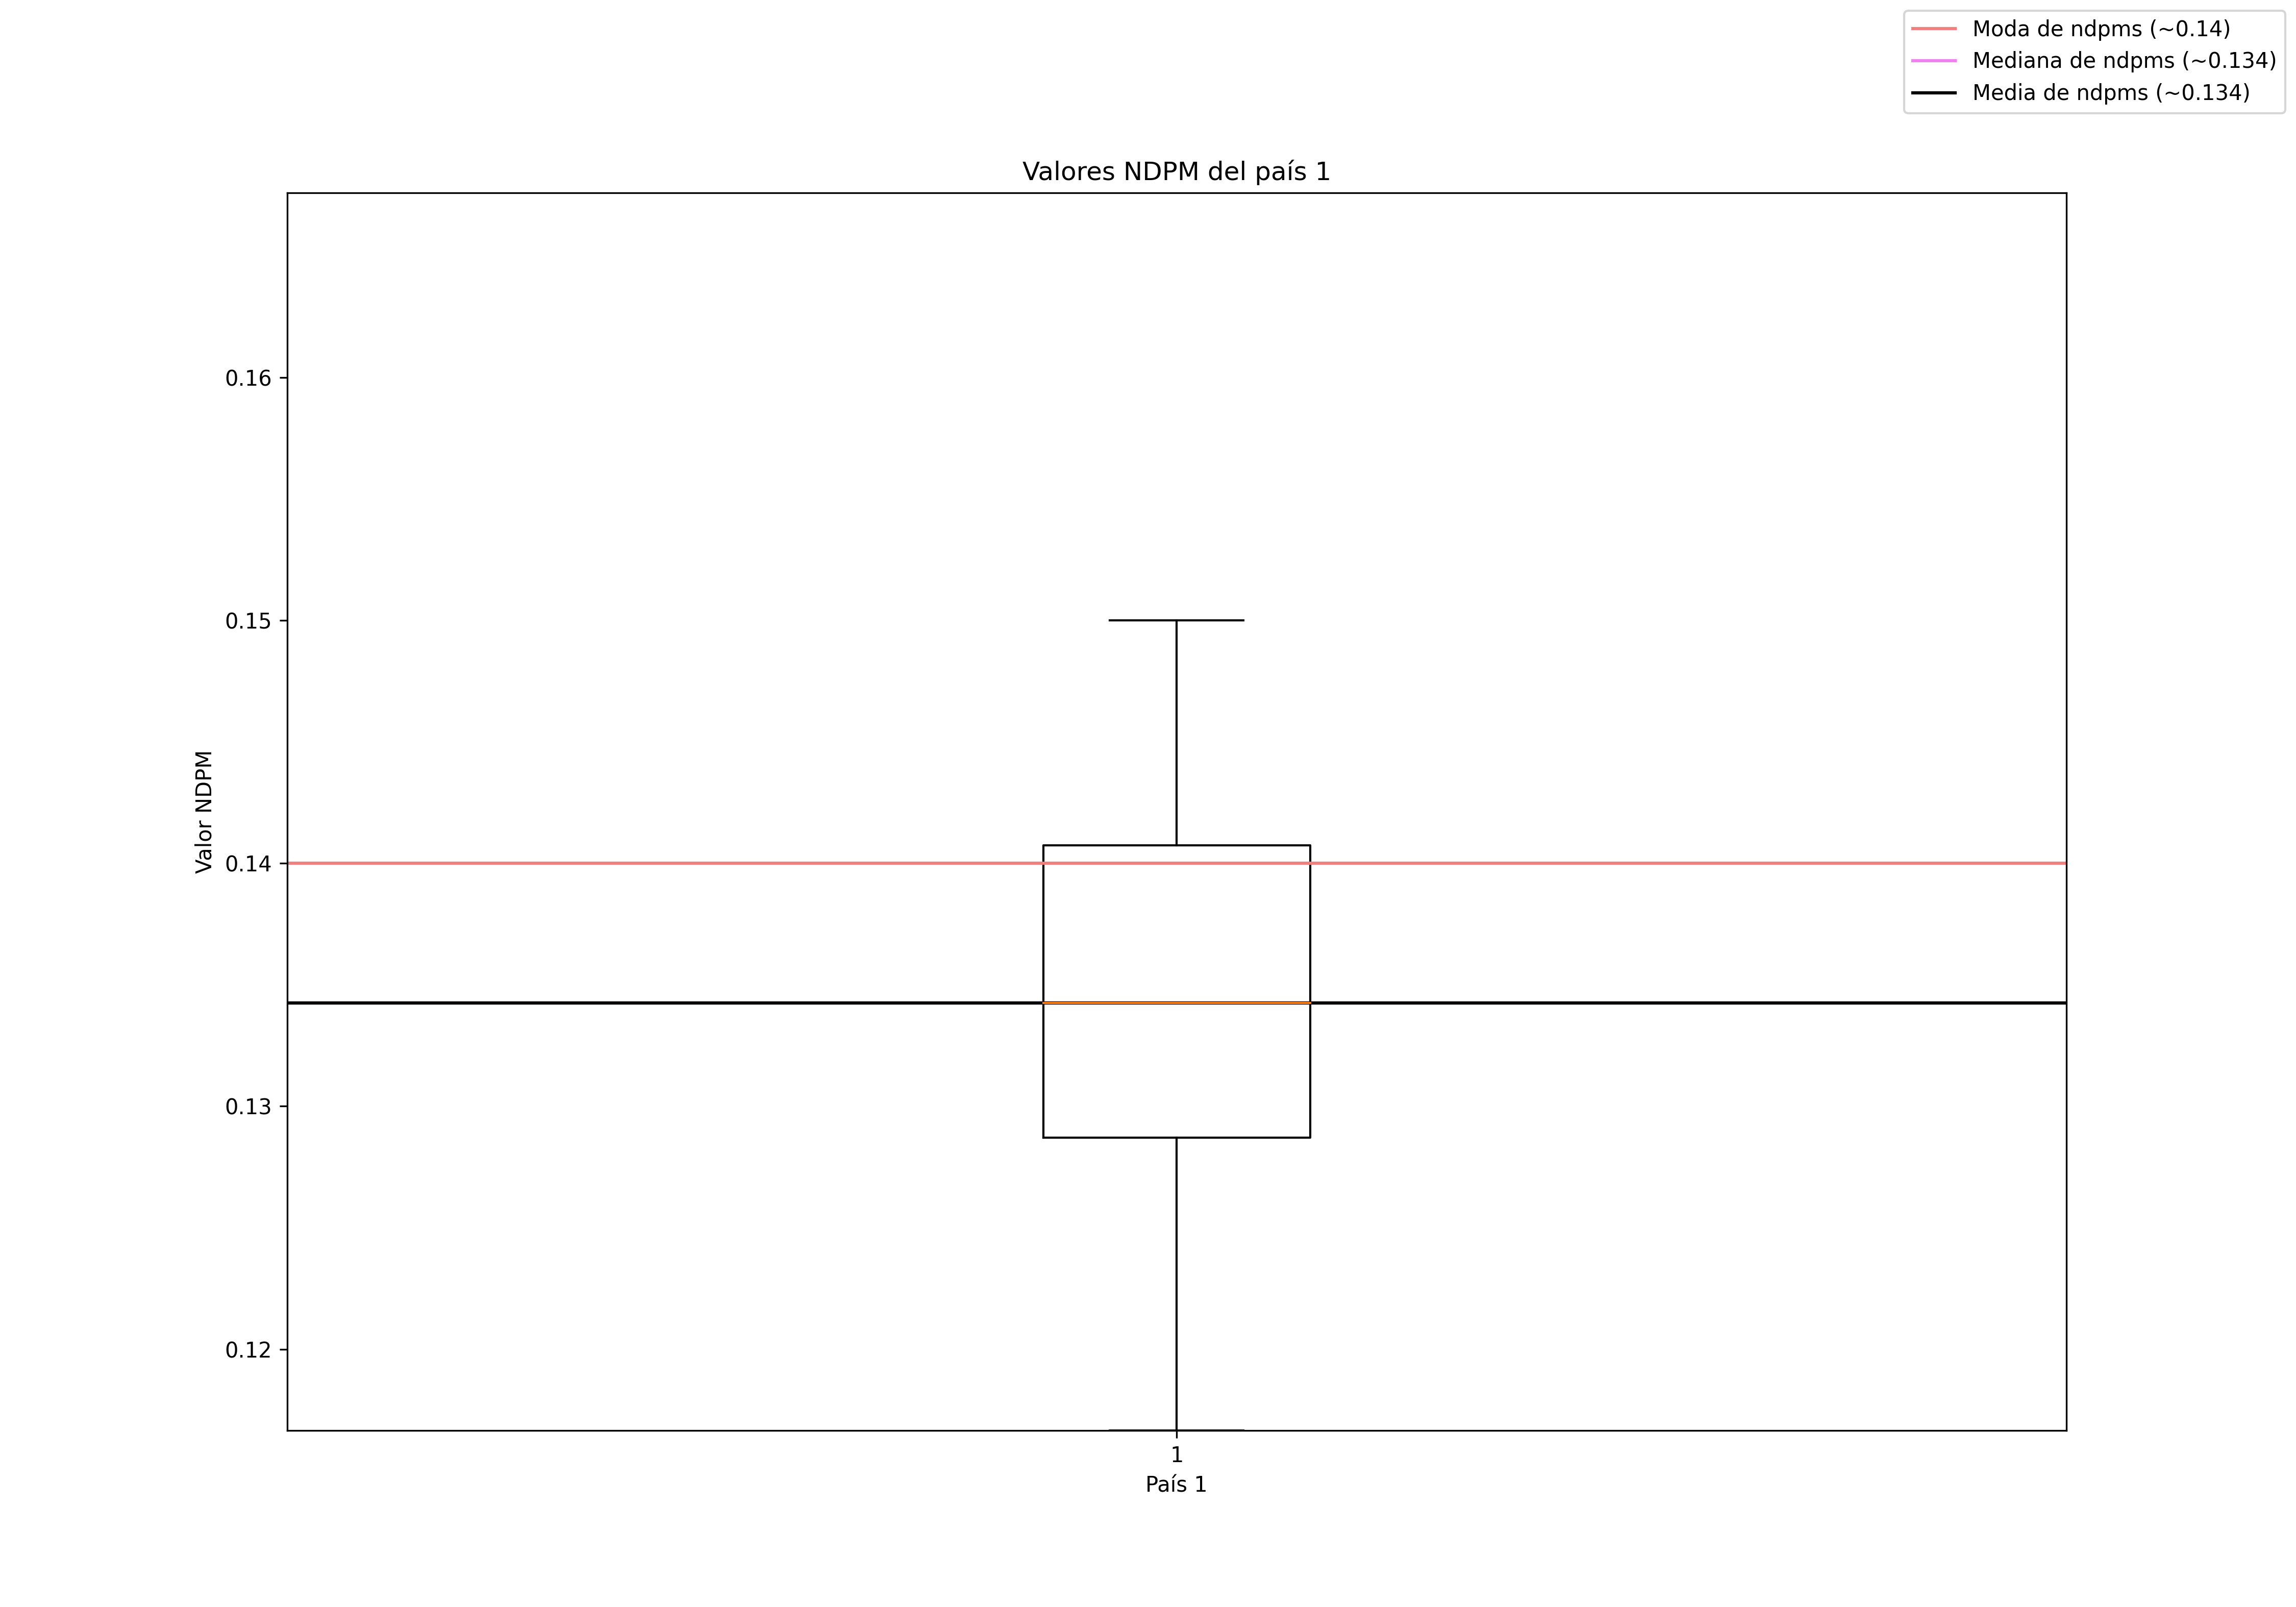
\includegraphics[width=0.5\textheight]
        {Figuras/Reports/PI_1_W0_LOC_CAJAS.png}}
        \quad
    \subfloat[Reentrenado con \textit{W$_c$ $=0$}]
        {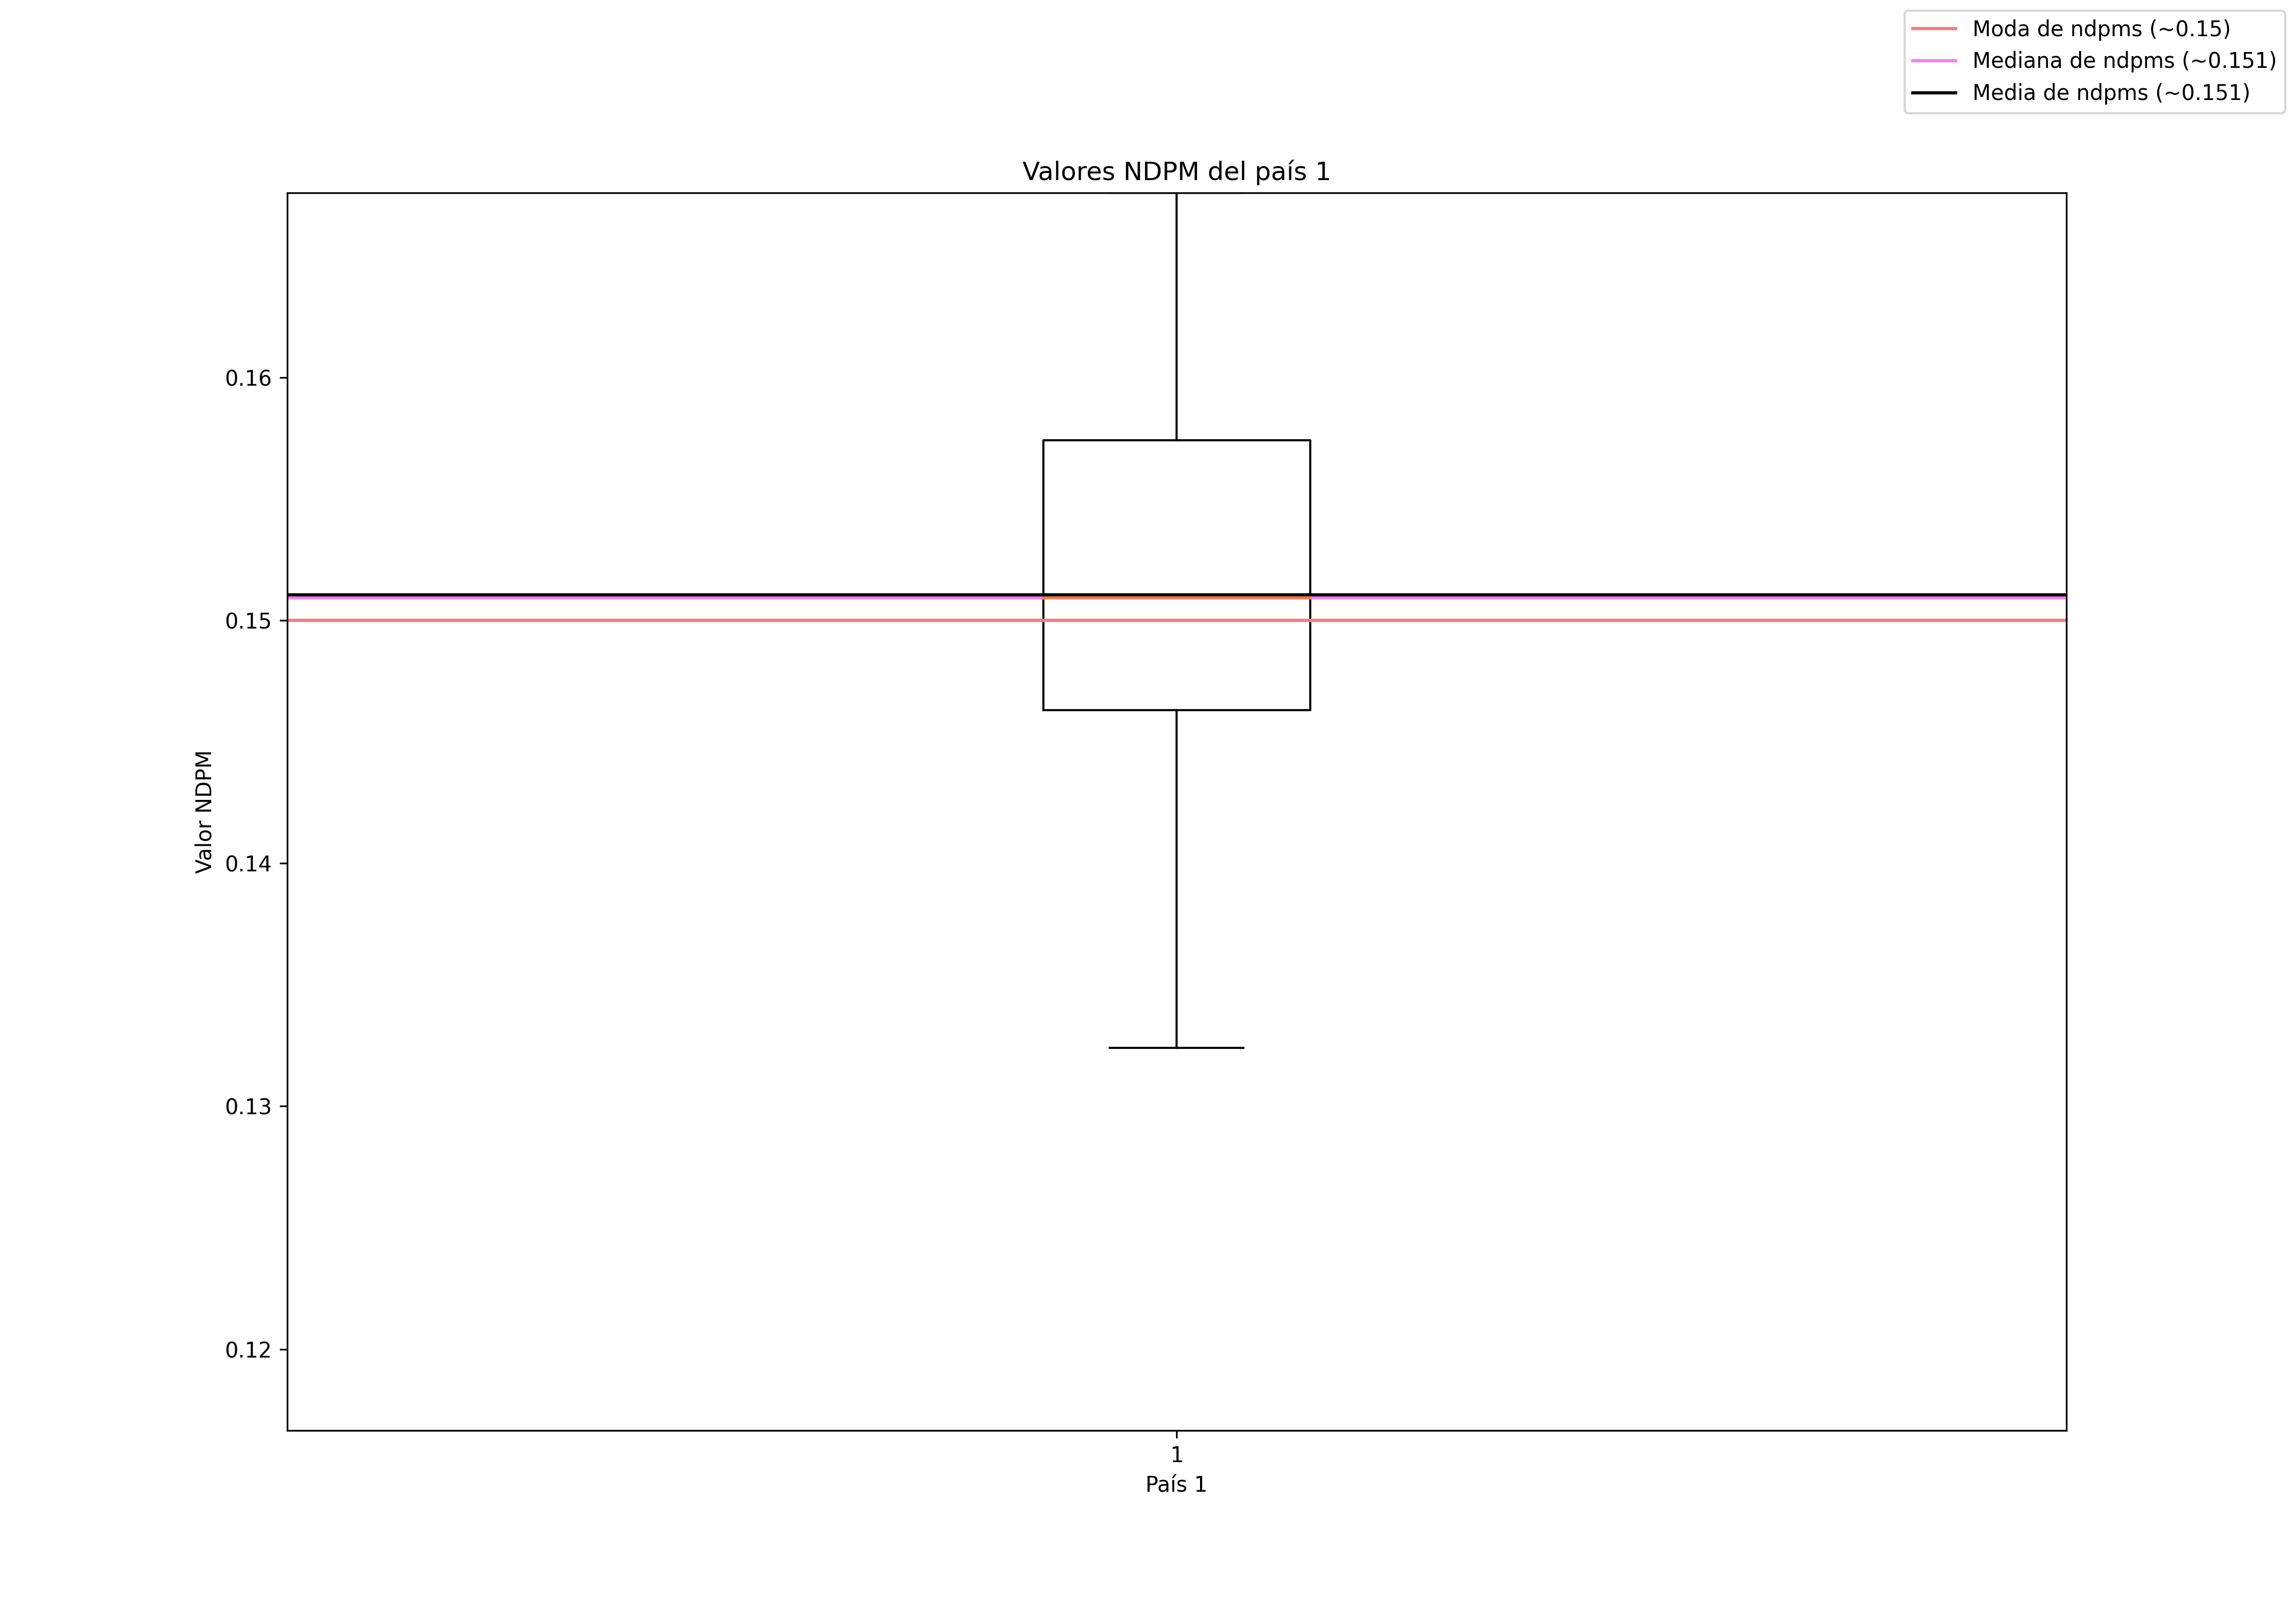
\includegraphics[width=0.5\textheight]
        {Figuras/Reports/PI_1_W0_EXT_CAJAS.png}}
    \subfloat[Reentrenado con \textit{W$_c$ $=1$}]{
        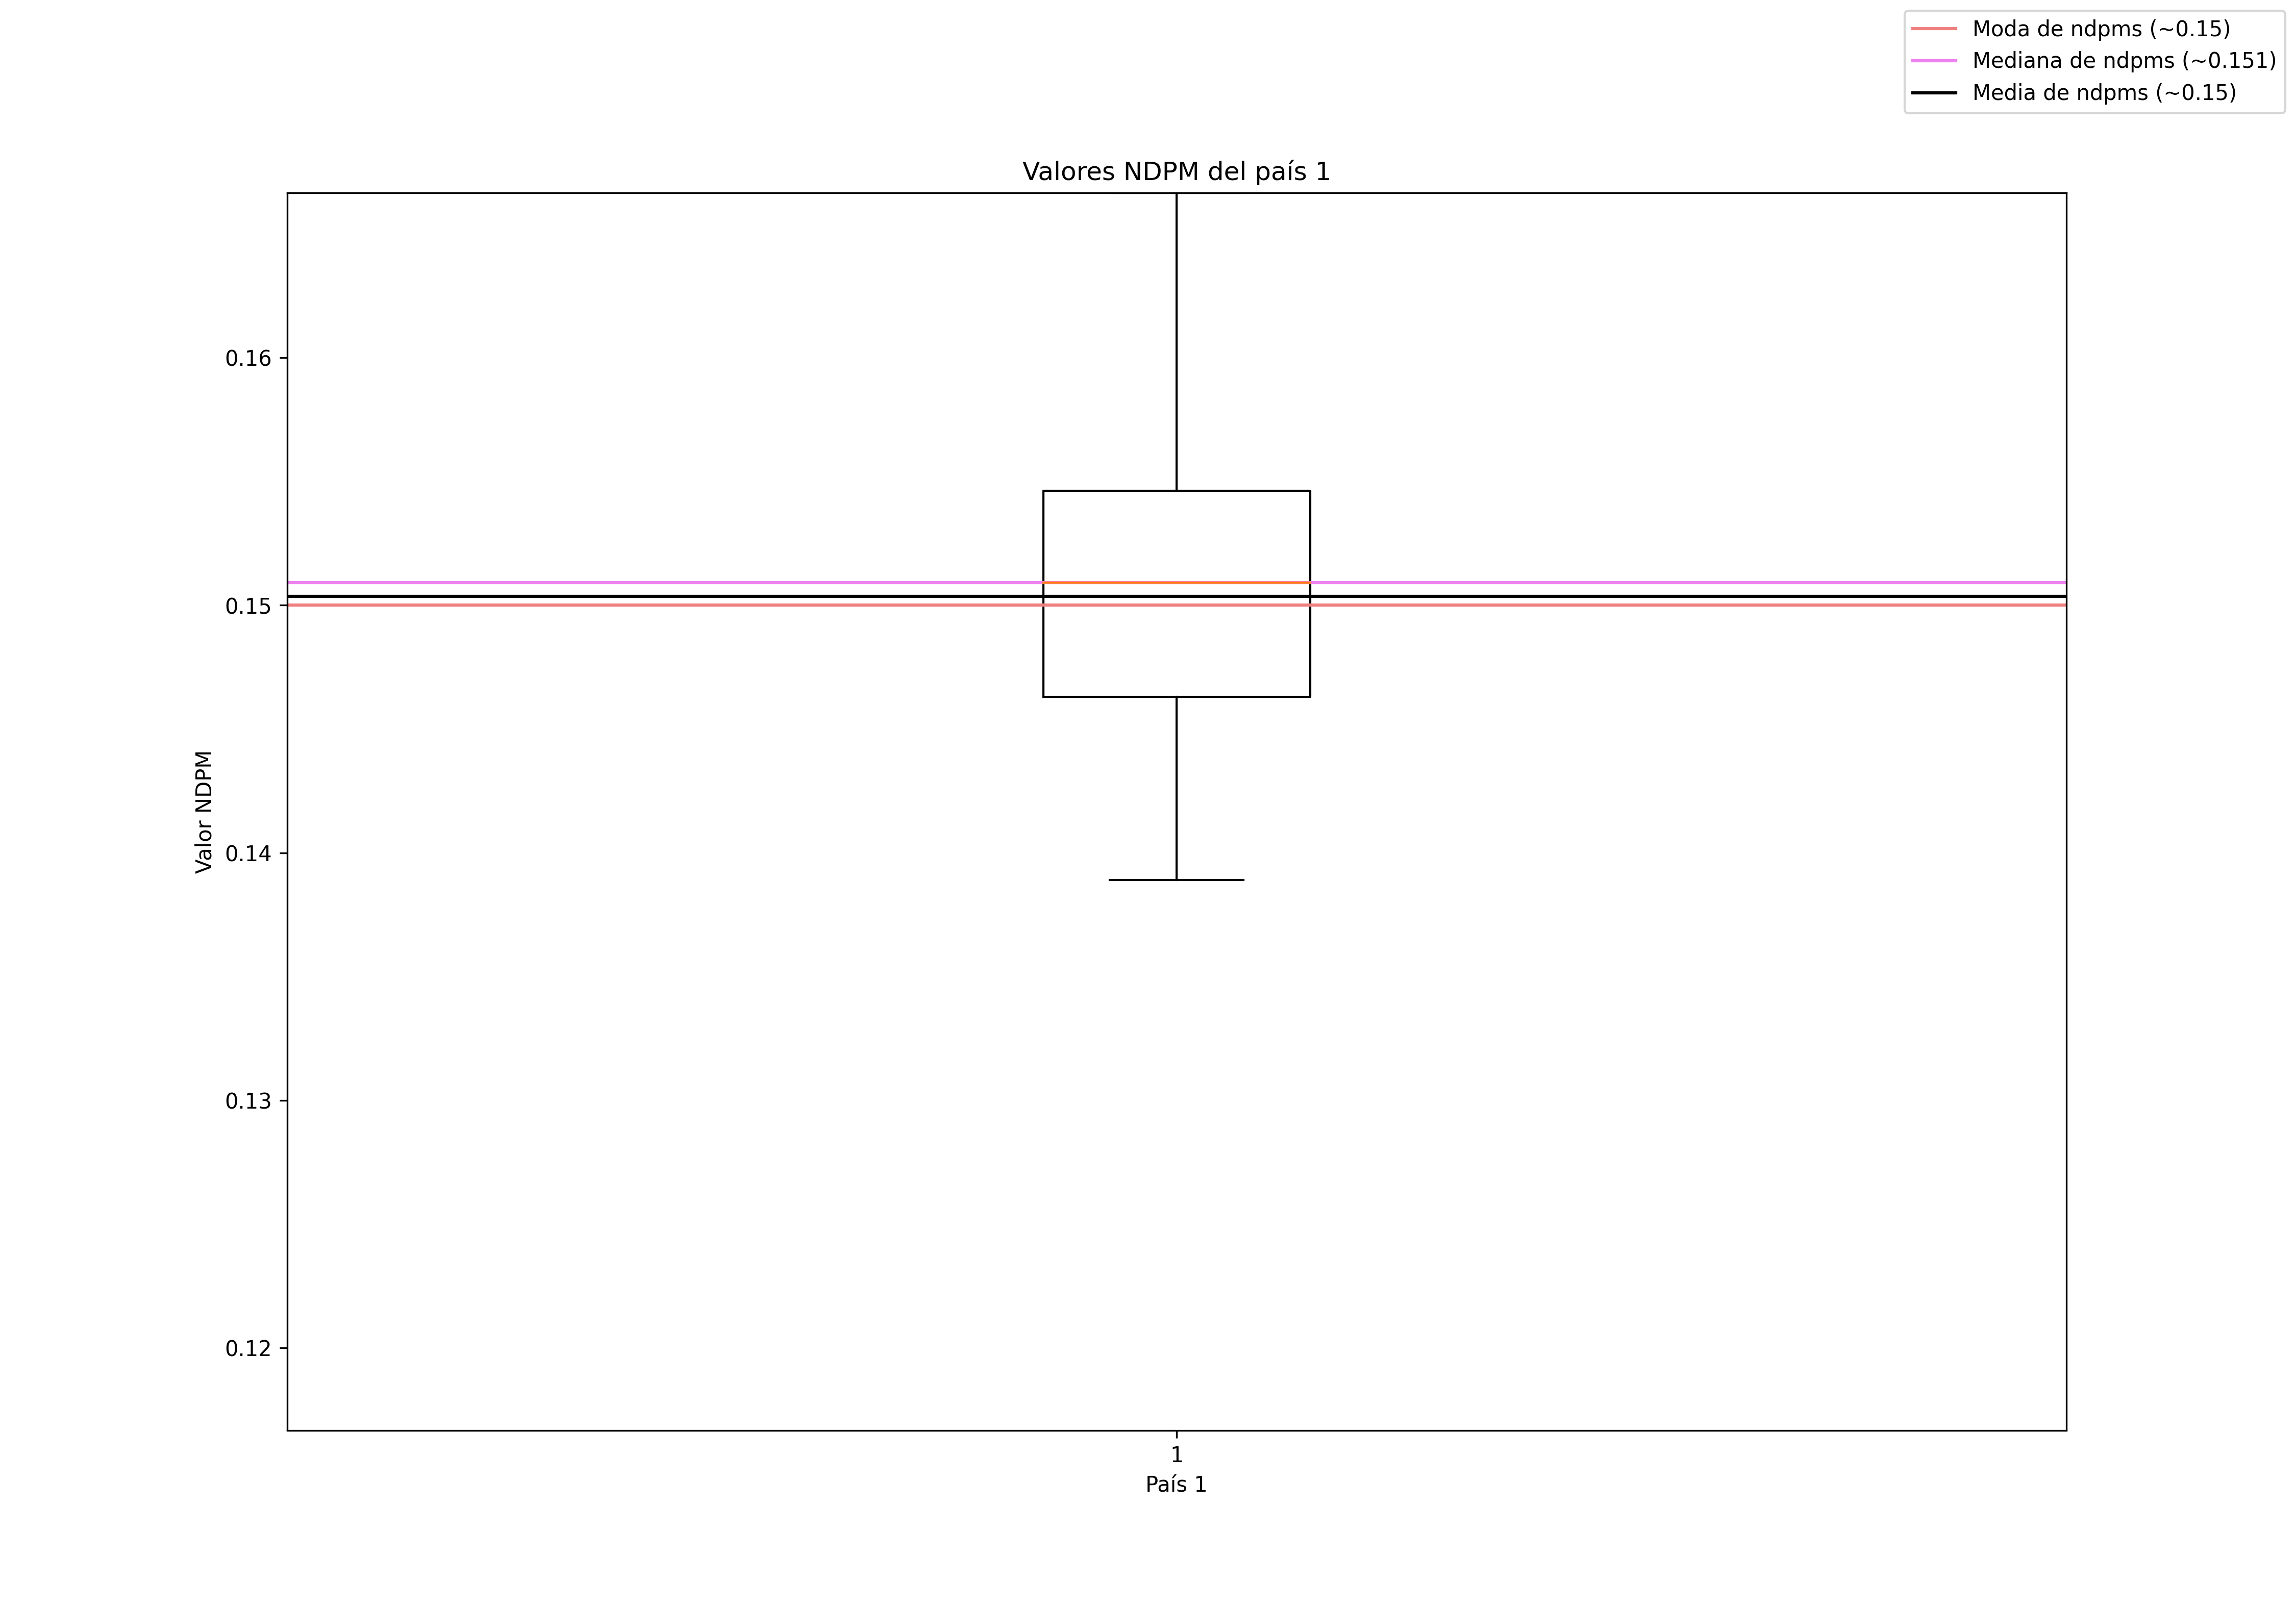
\includegraphics[width=0.5\textheight]
        {Figuras/Reports/PI_1_W1_EXT_CAJAS.png}}
    \caption{Diagramas de cajas y bigotes de los valores NDPM del participante 1\label{fig:PI1_CAJAS}}
\end{sidewaysfigure}
\clearpage
\begin{sidewaysfigure}
    \centering
    \subfloat[Modelo original]
        {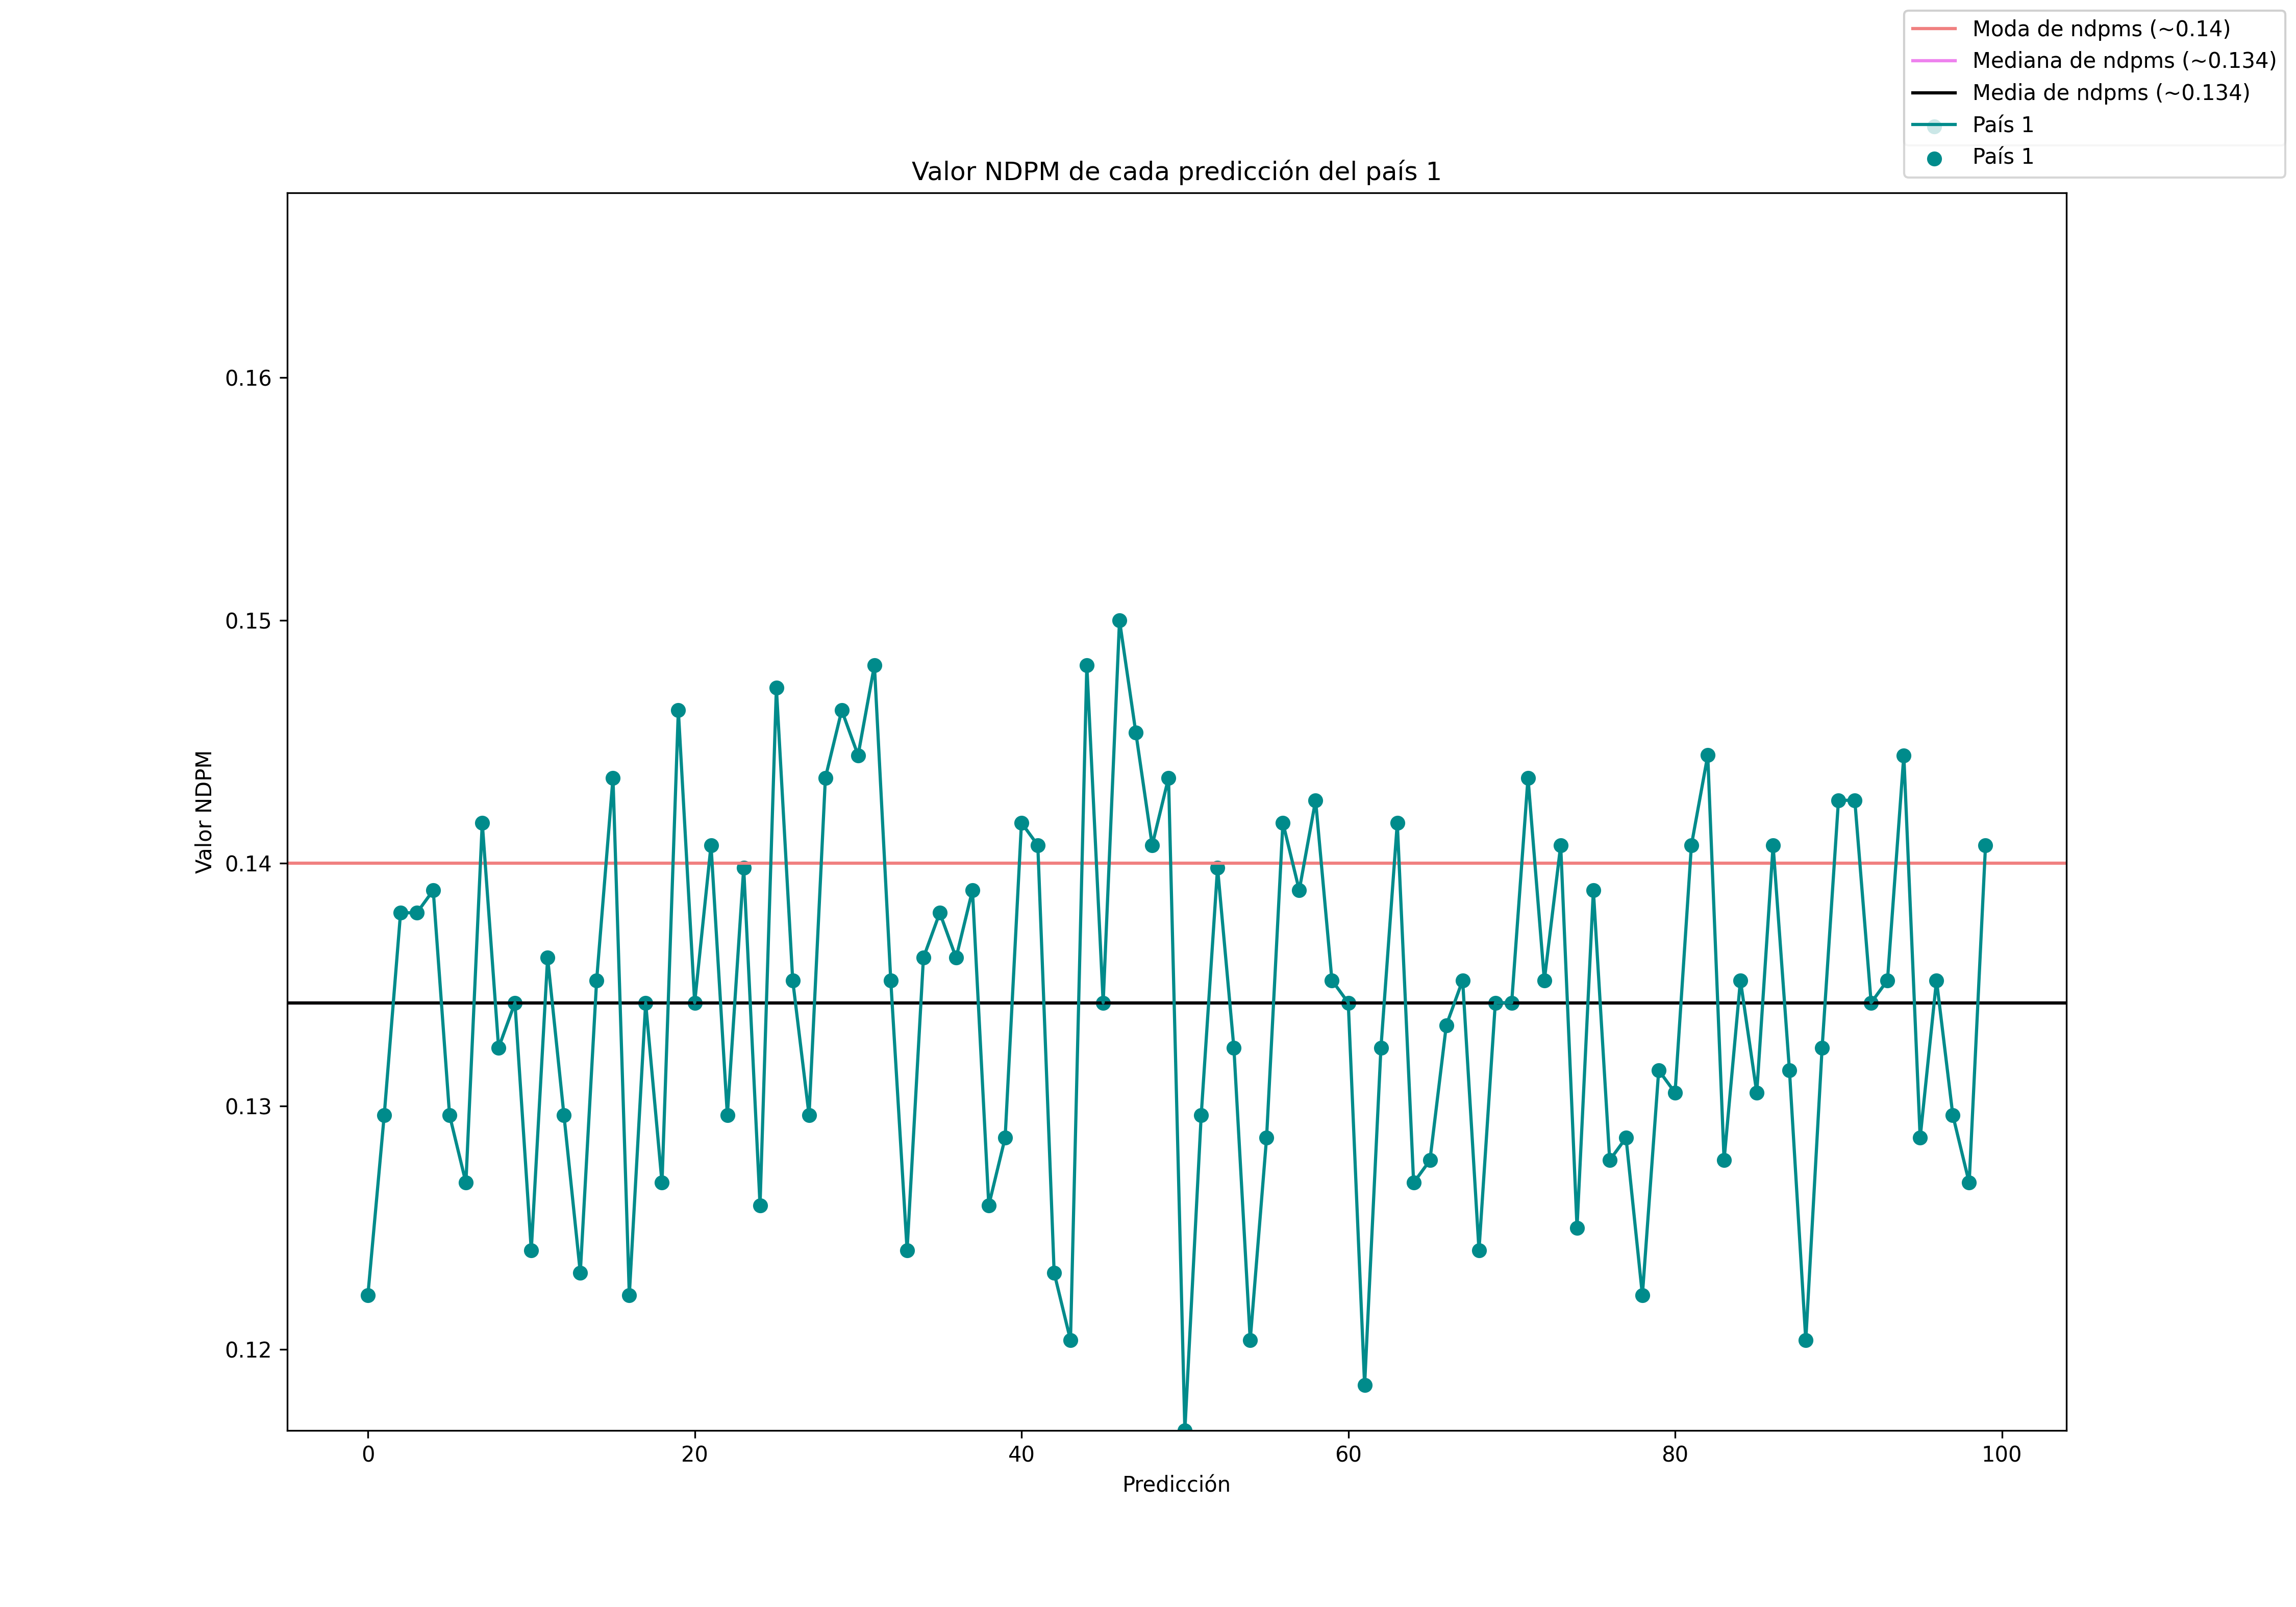
\includegraphics[width=0.5\textheight]
        {Figuras/Reports/PI_1_W0_LOC_DISP.png}}
        \quad
    \subfloat[Reentrenado con \textit{W$_c$ $=0$}]
        {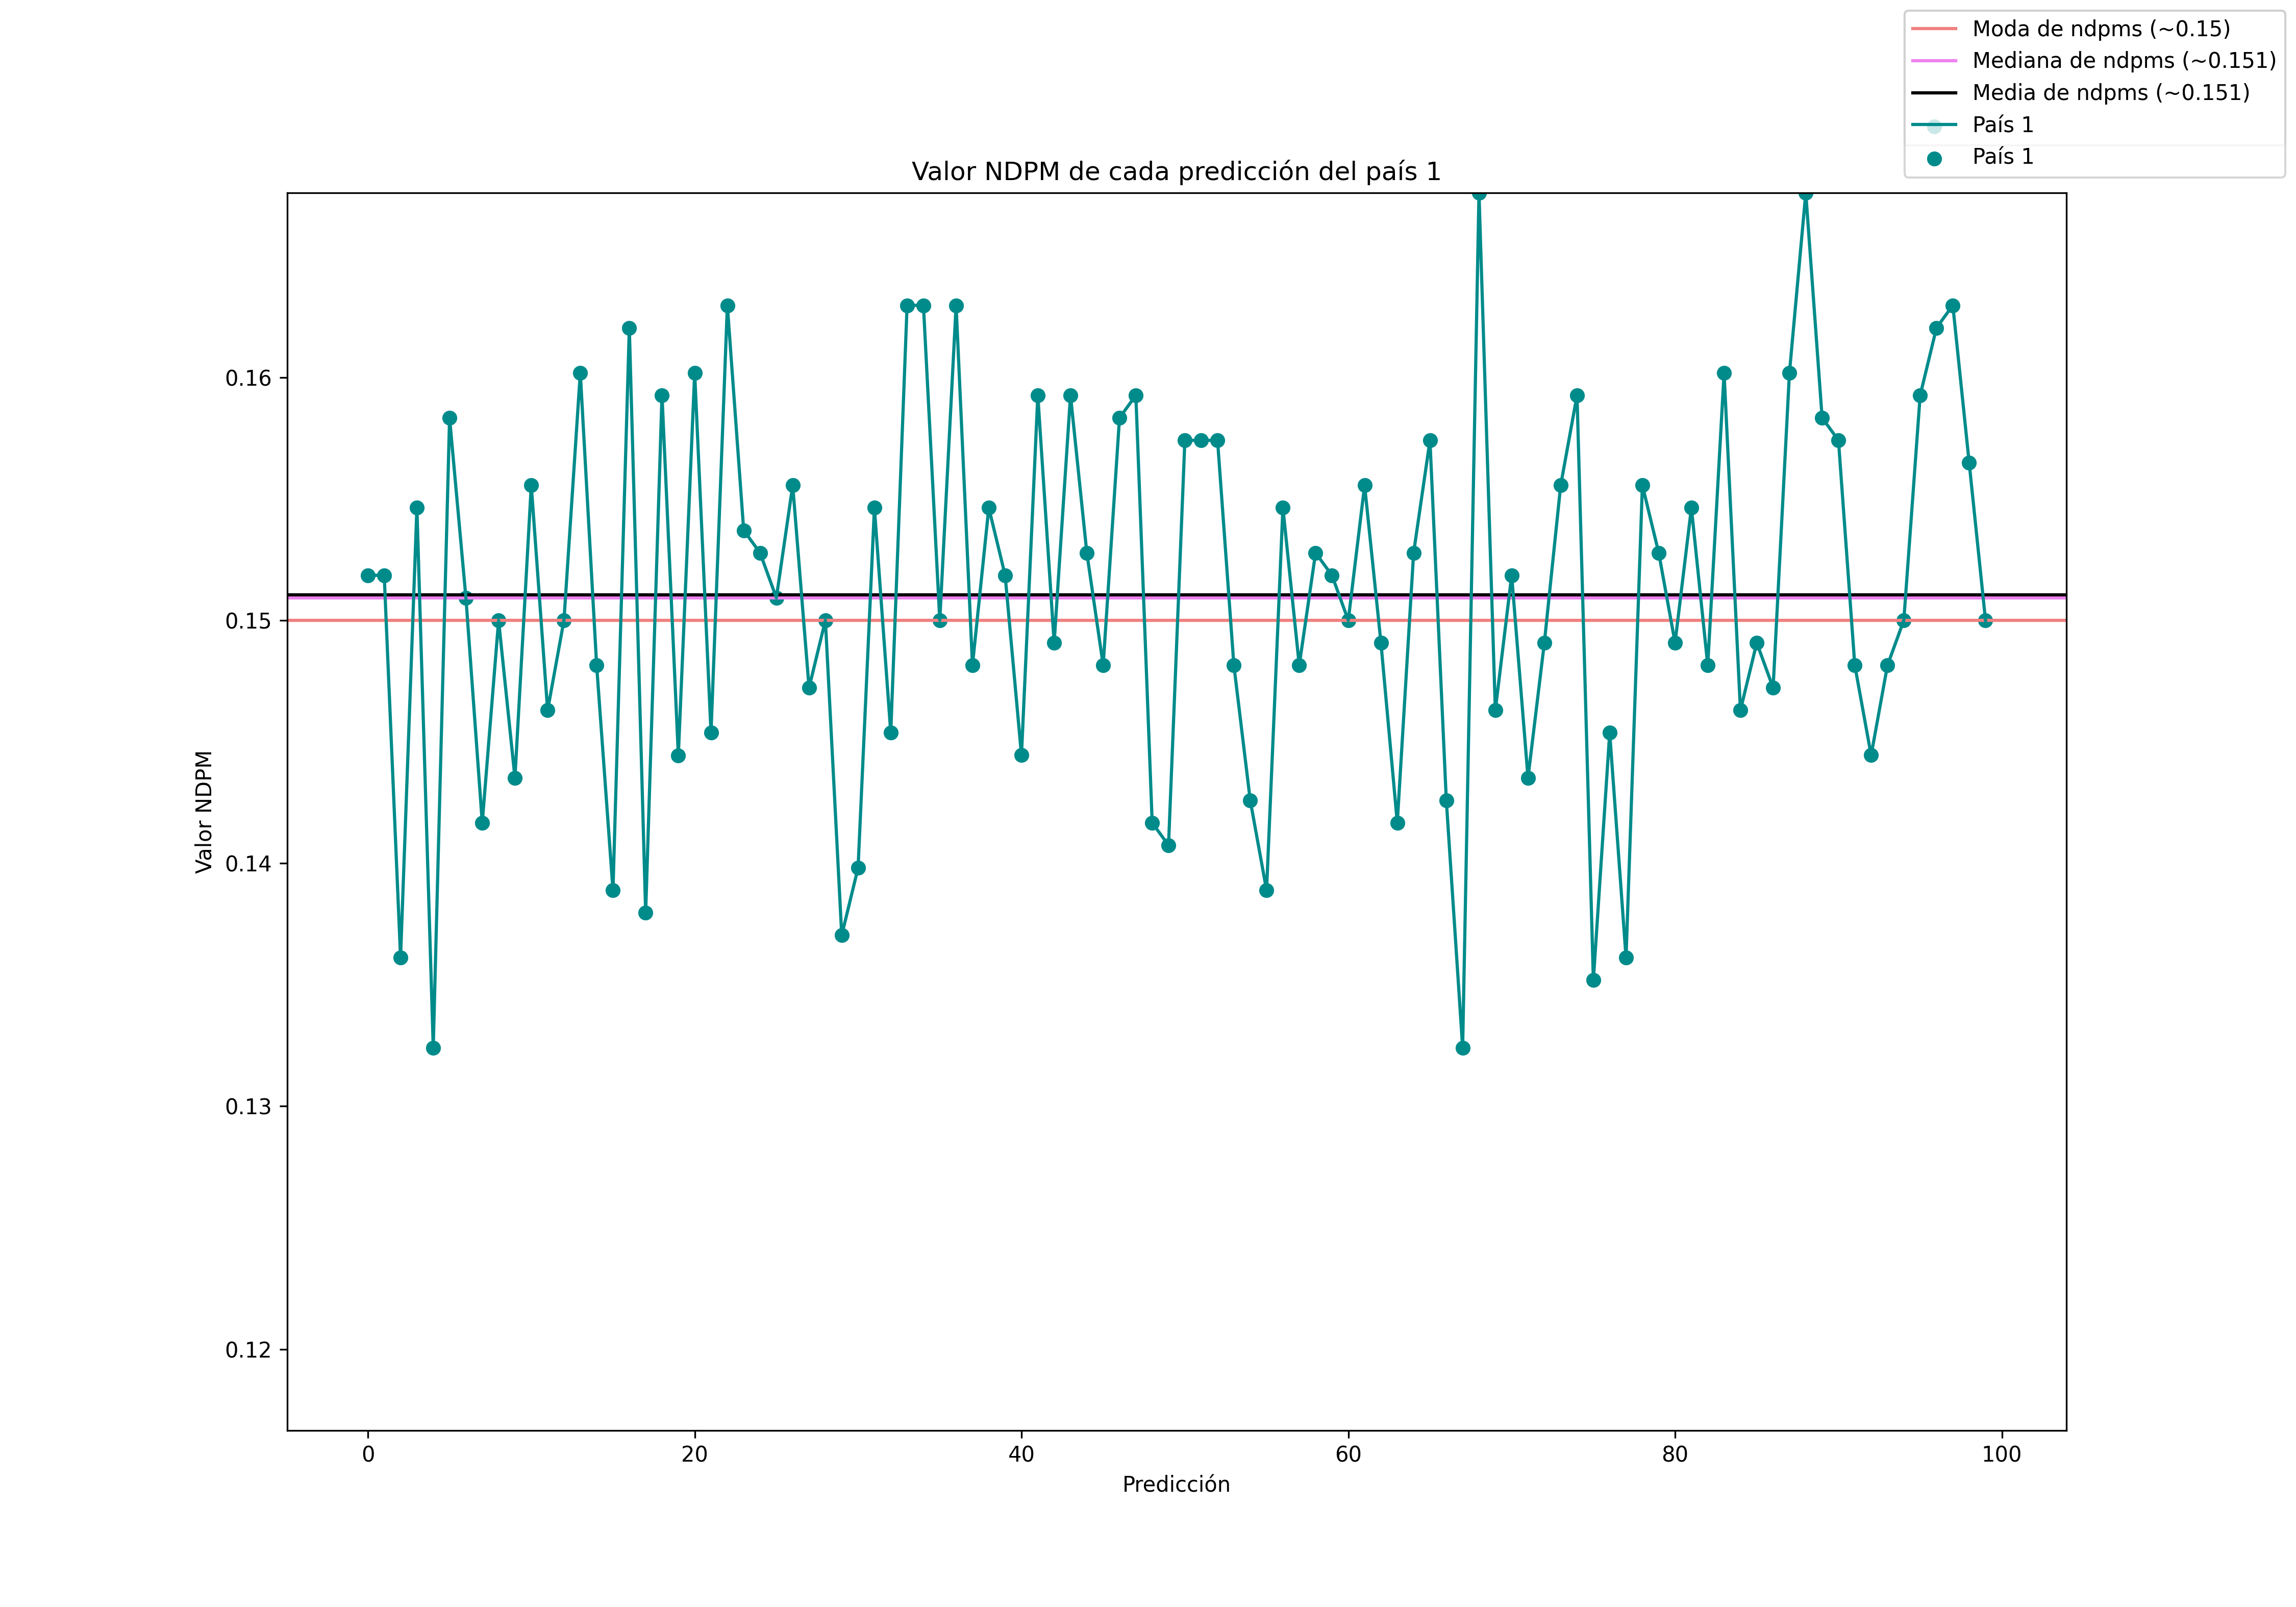
\includegraphics[width=0.5\textheight]
        {Figuras/Reports/PI_1_W0_EXT_DISP.png}}
    \subfloat[Reentrenado con \textit{W$_c$ $=1$}]{
        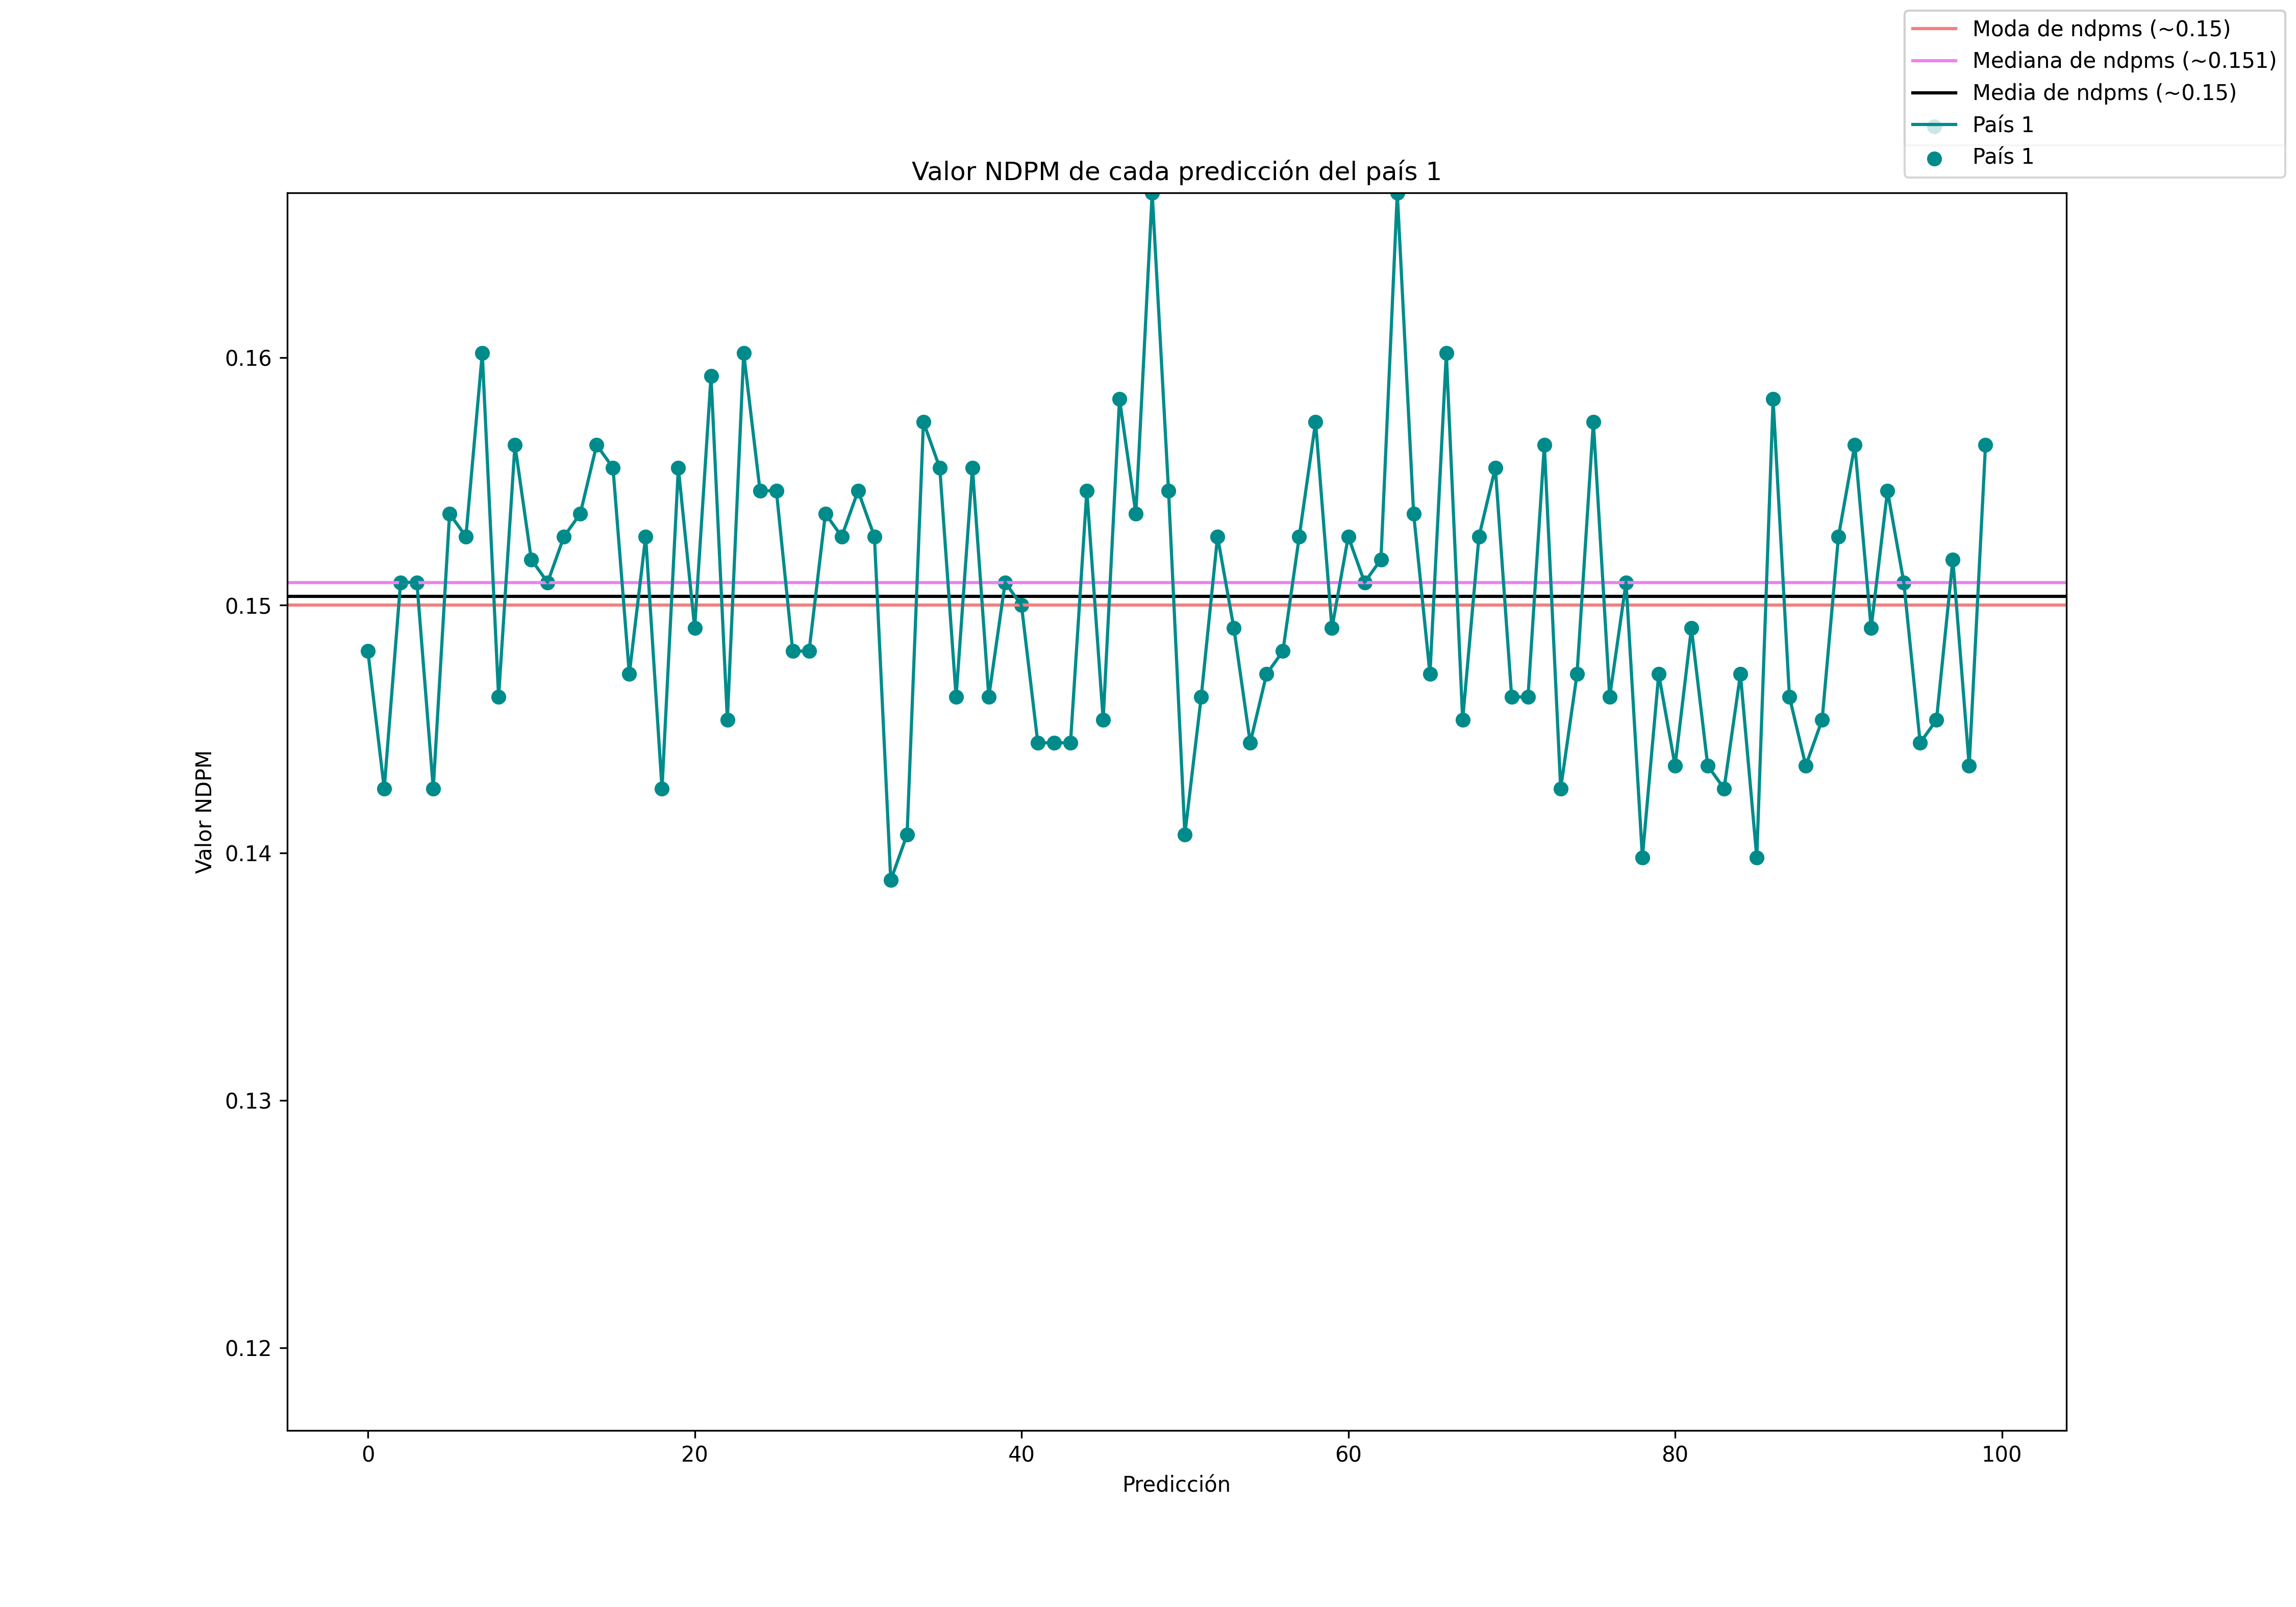
\includegraphics[width=0.5\textheight]
        {Figuras/Reports/PI_1_W1_EXT_DISP.png}}
    \caption{Gráfico de los valores NDPM del participante 1\label{fig:PI1_DISP}}
\end{sidewaysfigure}
\clearpage

\begin{sidewaysfigure}
    \centering
    \subfloat[Modelo original]
        {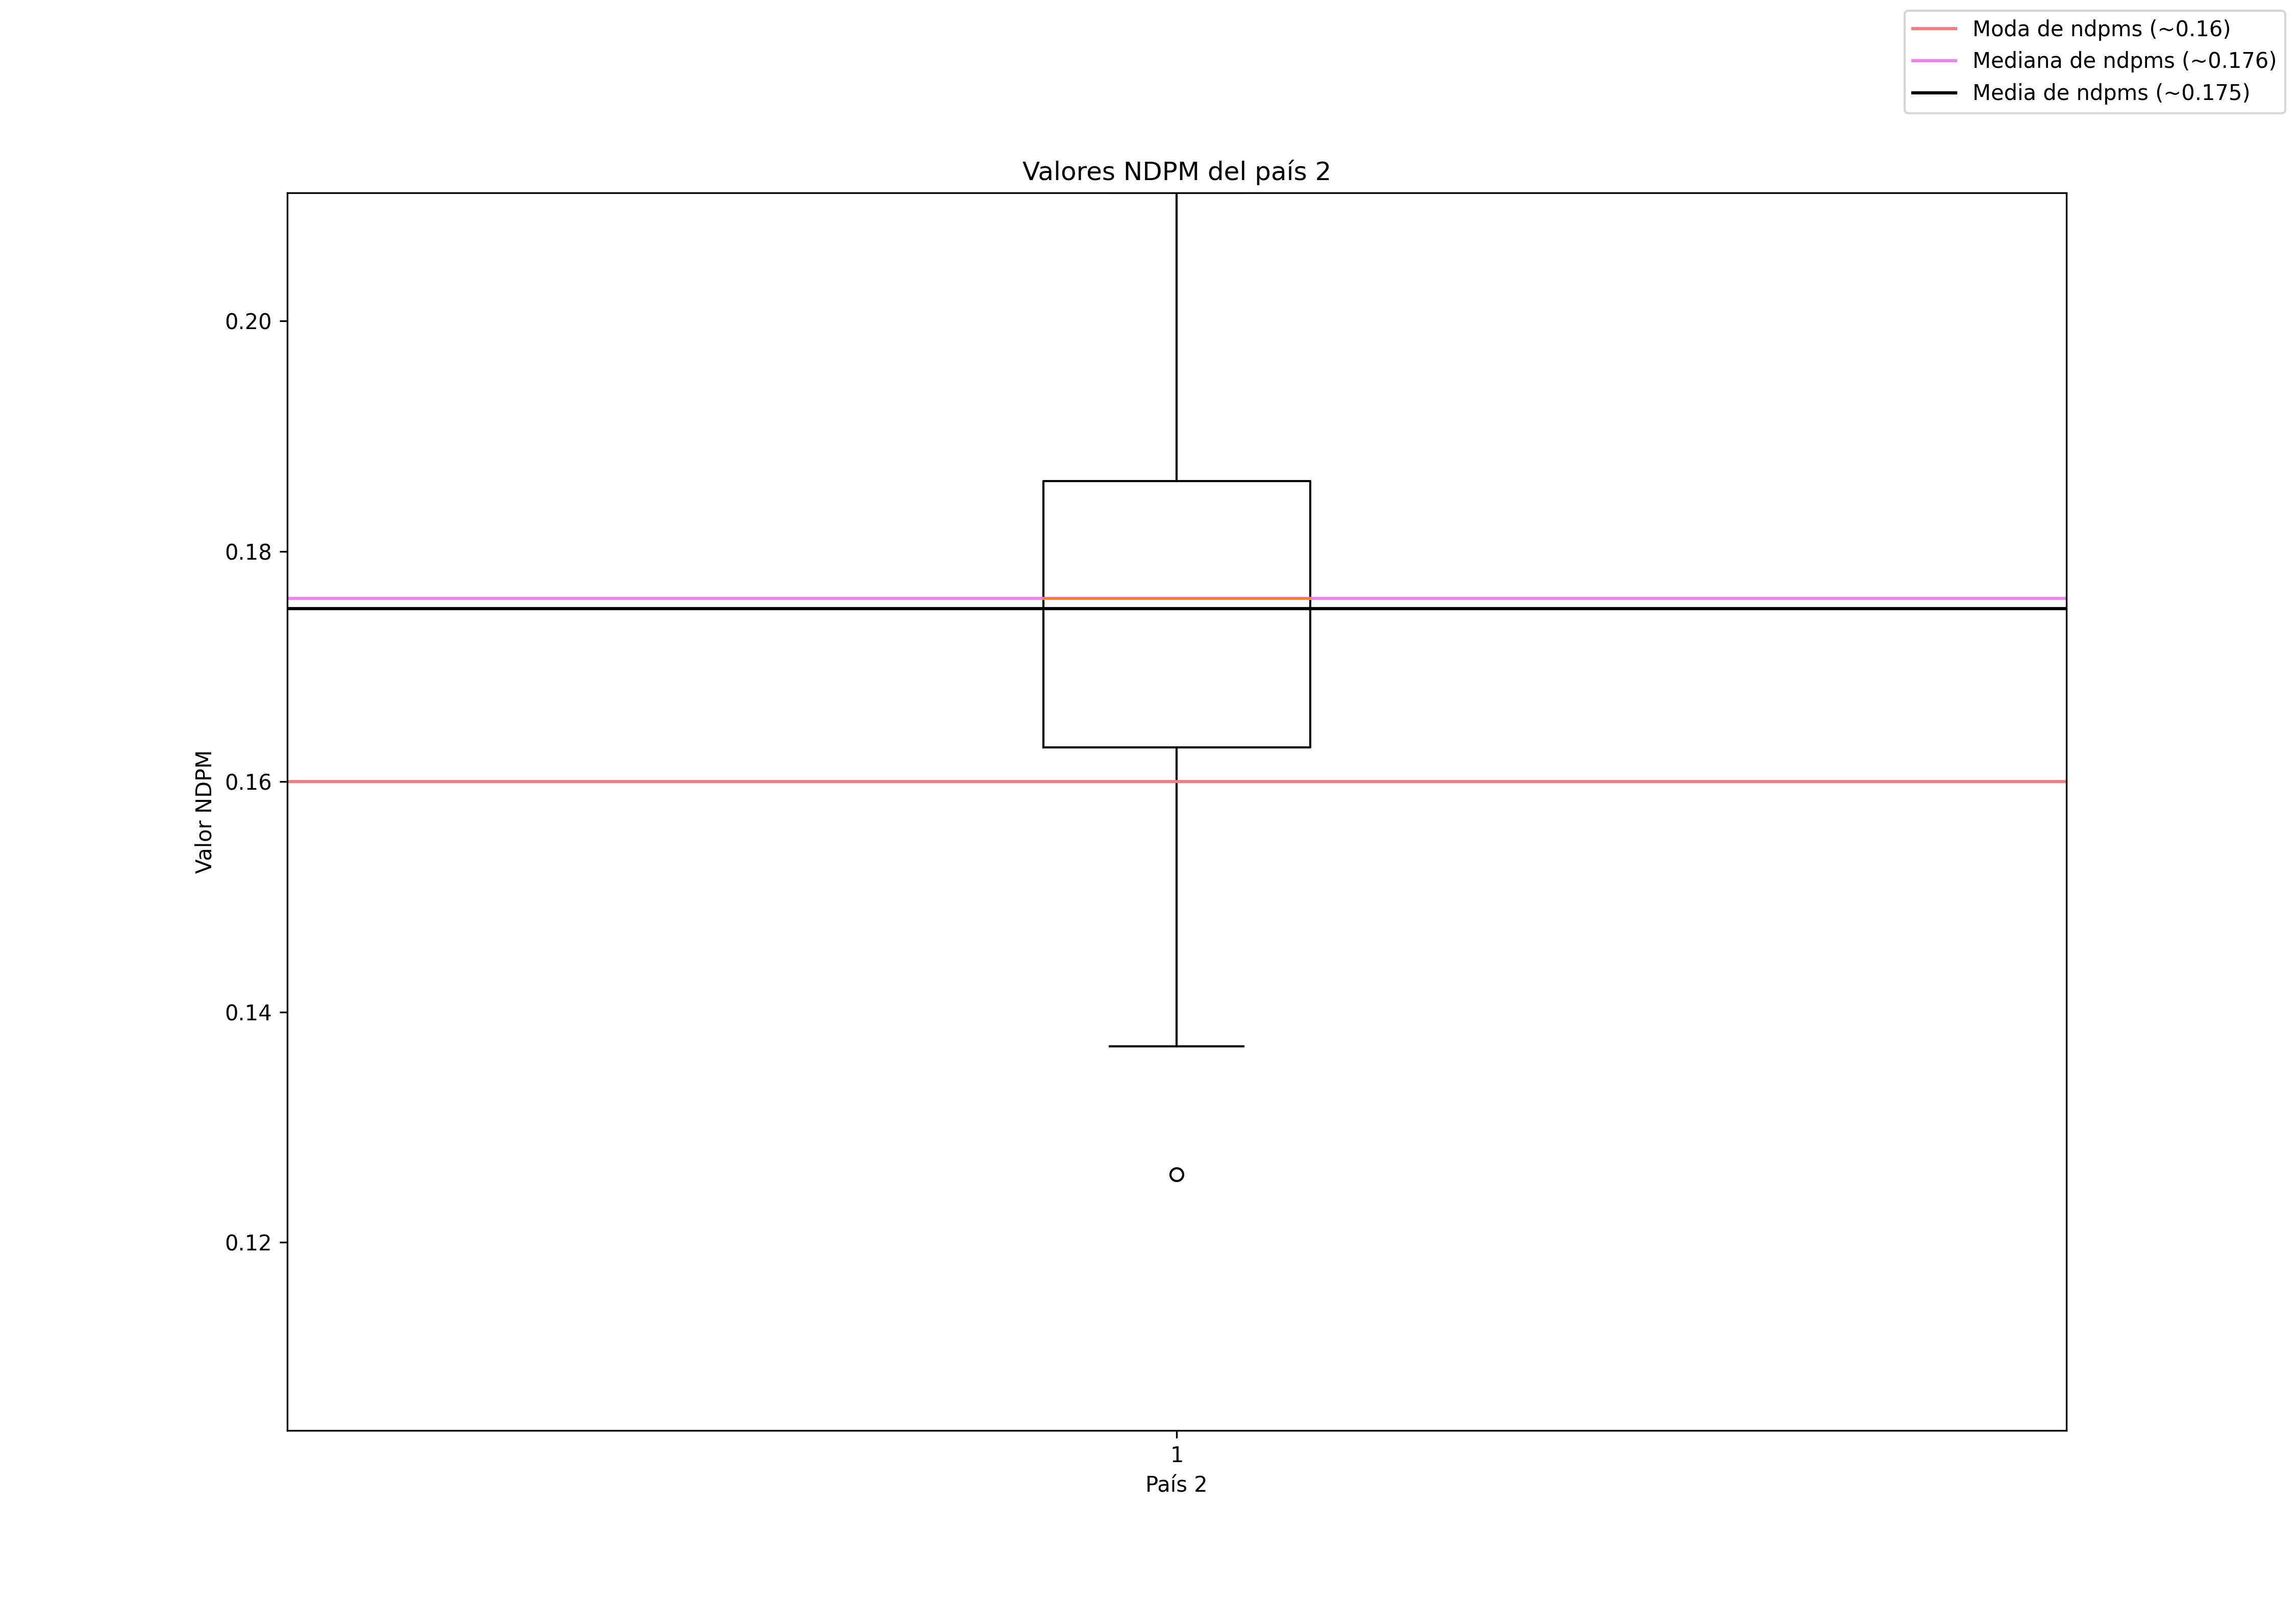
\includegraphics[width=0.5\textheight]
        {Figuras/Reports/PI_2_W0_LOC_CAJAS.png}}
        \quad
    \subfloat[Reentrenado con \textit{W$_c$ $=0$}]
        {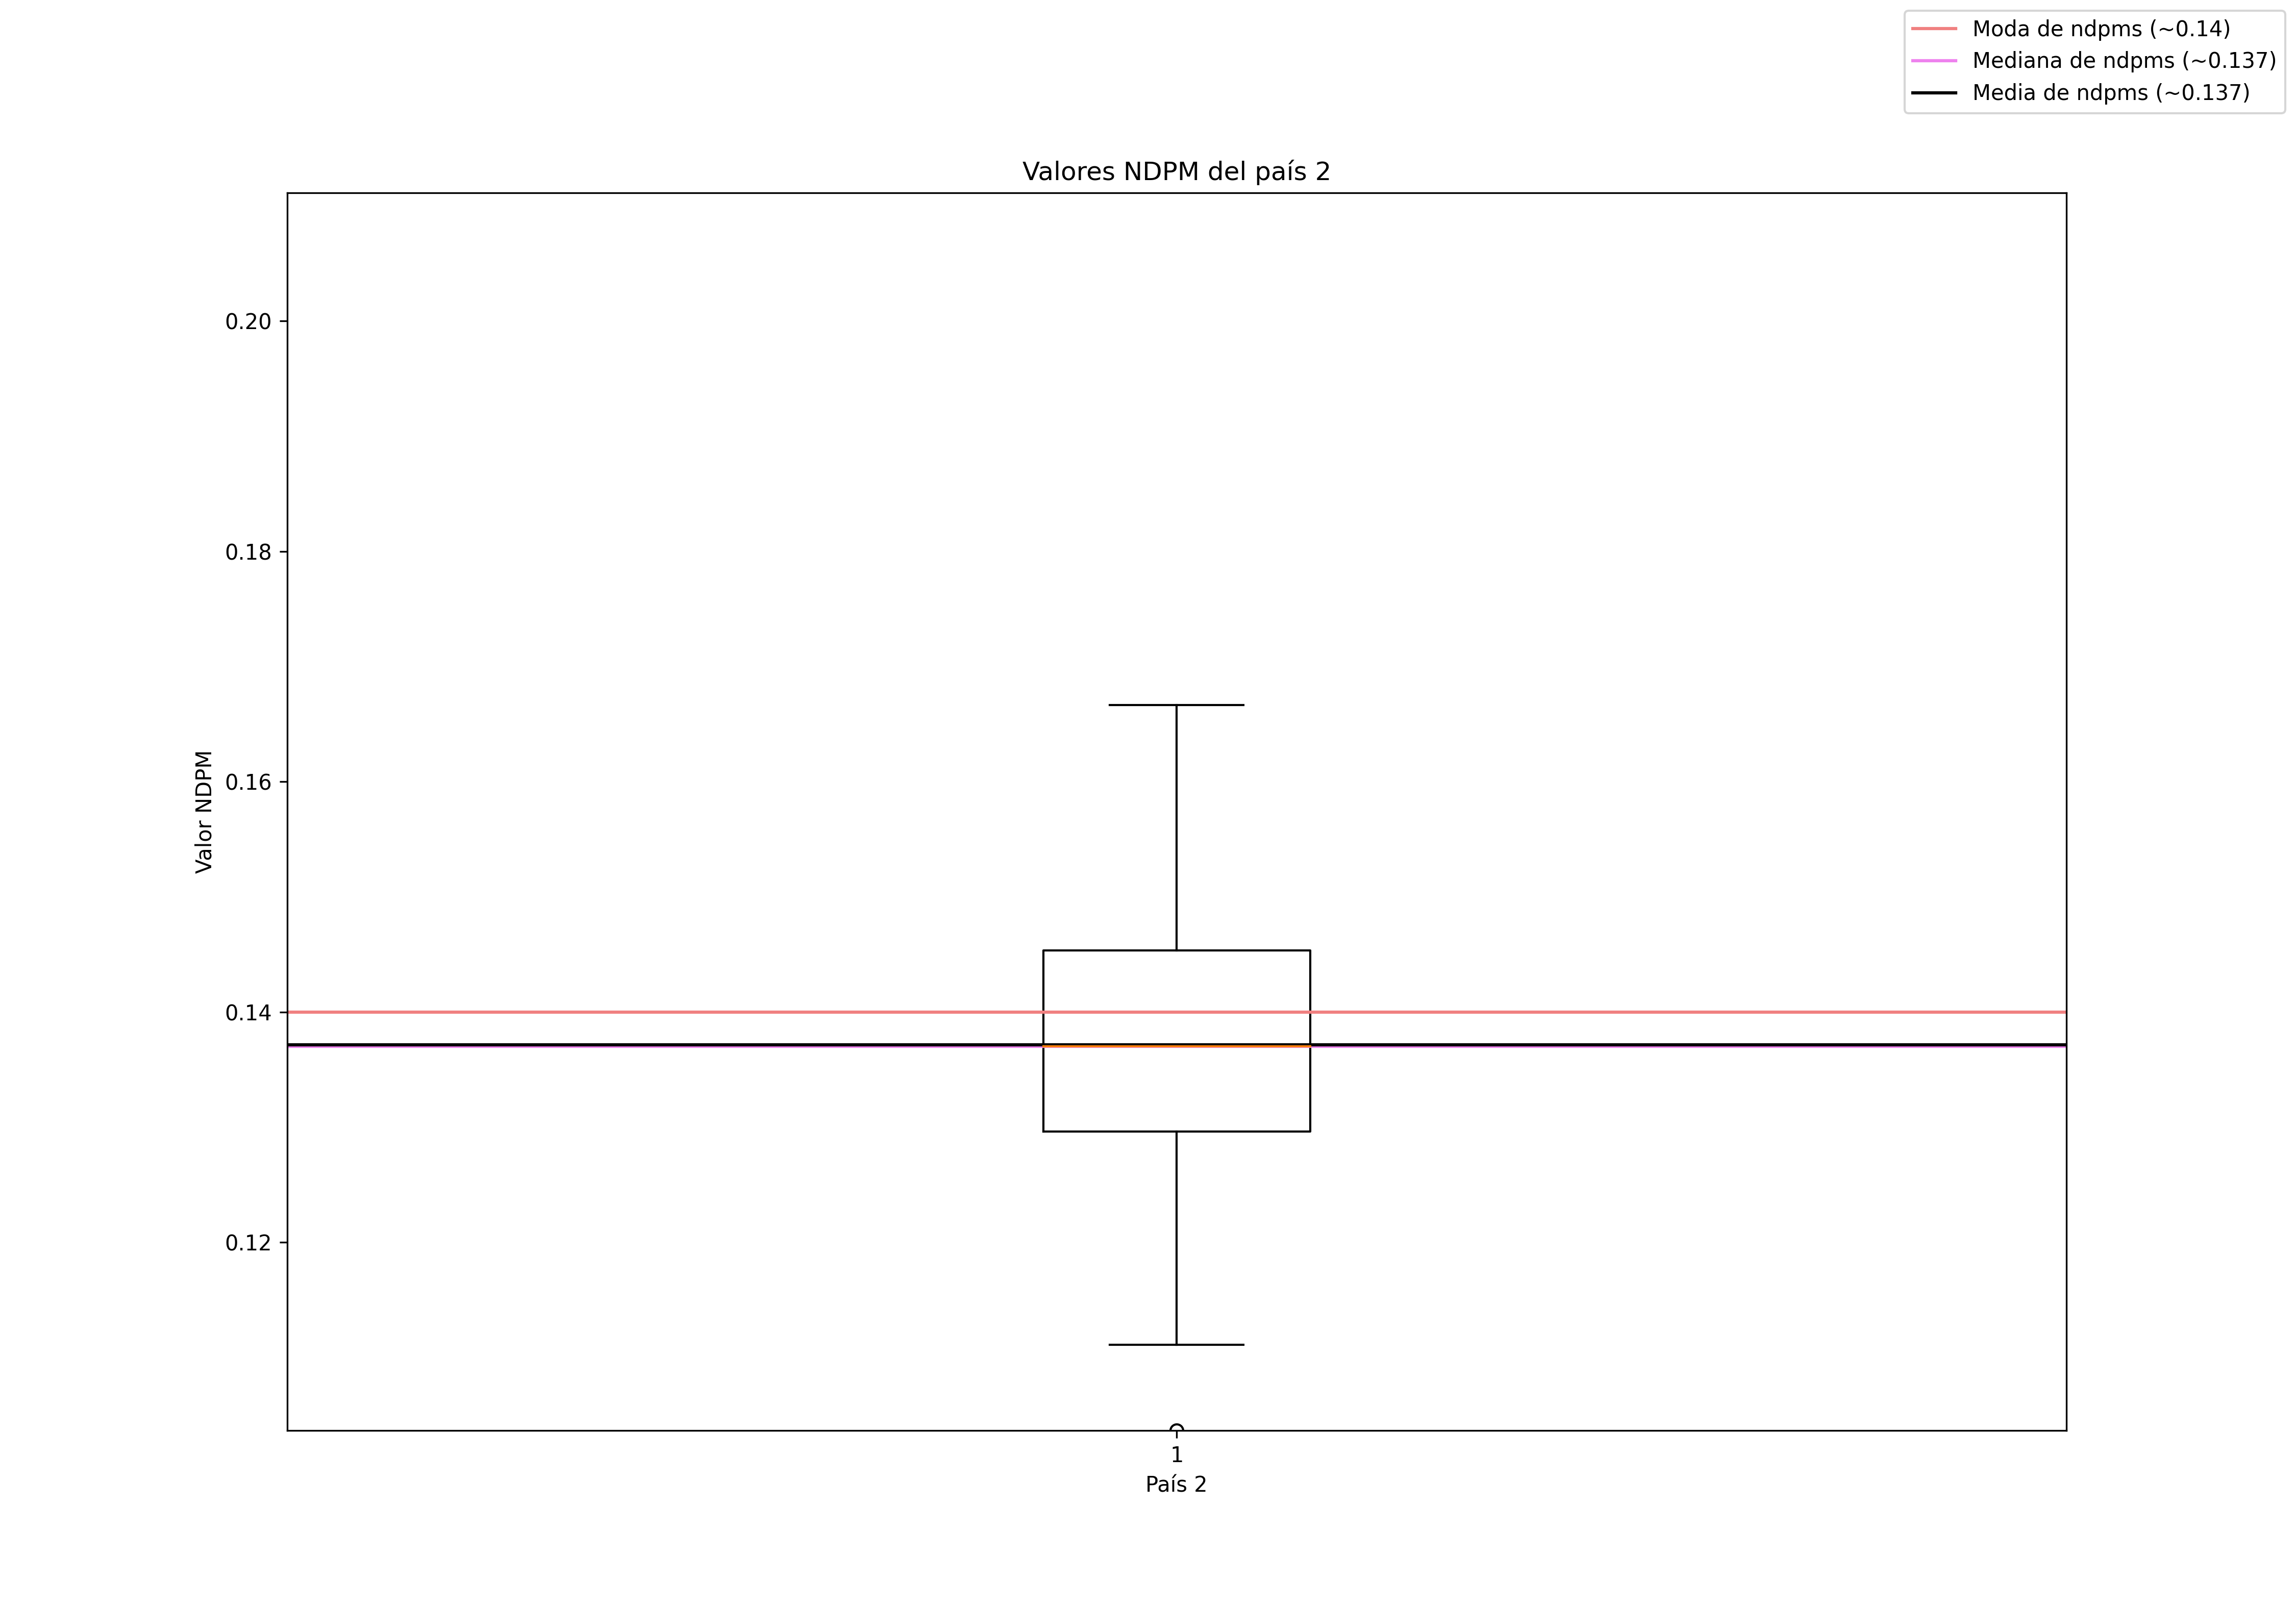
\includegraphics[width=0.5\textheight]
        {Figuras/Reports/PI_2_W0_EXT_CAJAS.png}}
    \subfloat[Reentrenado con \textit{W$_c$ $=1$}]{
        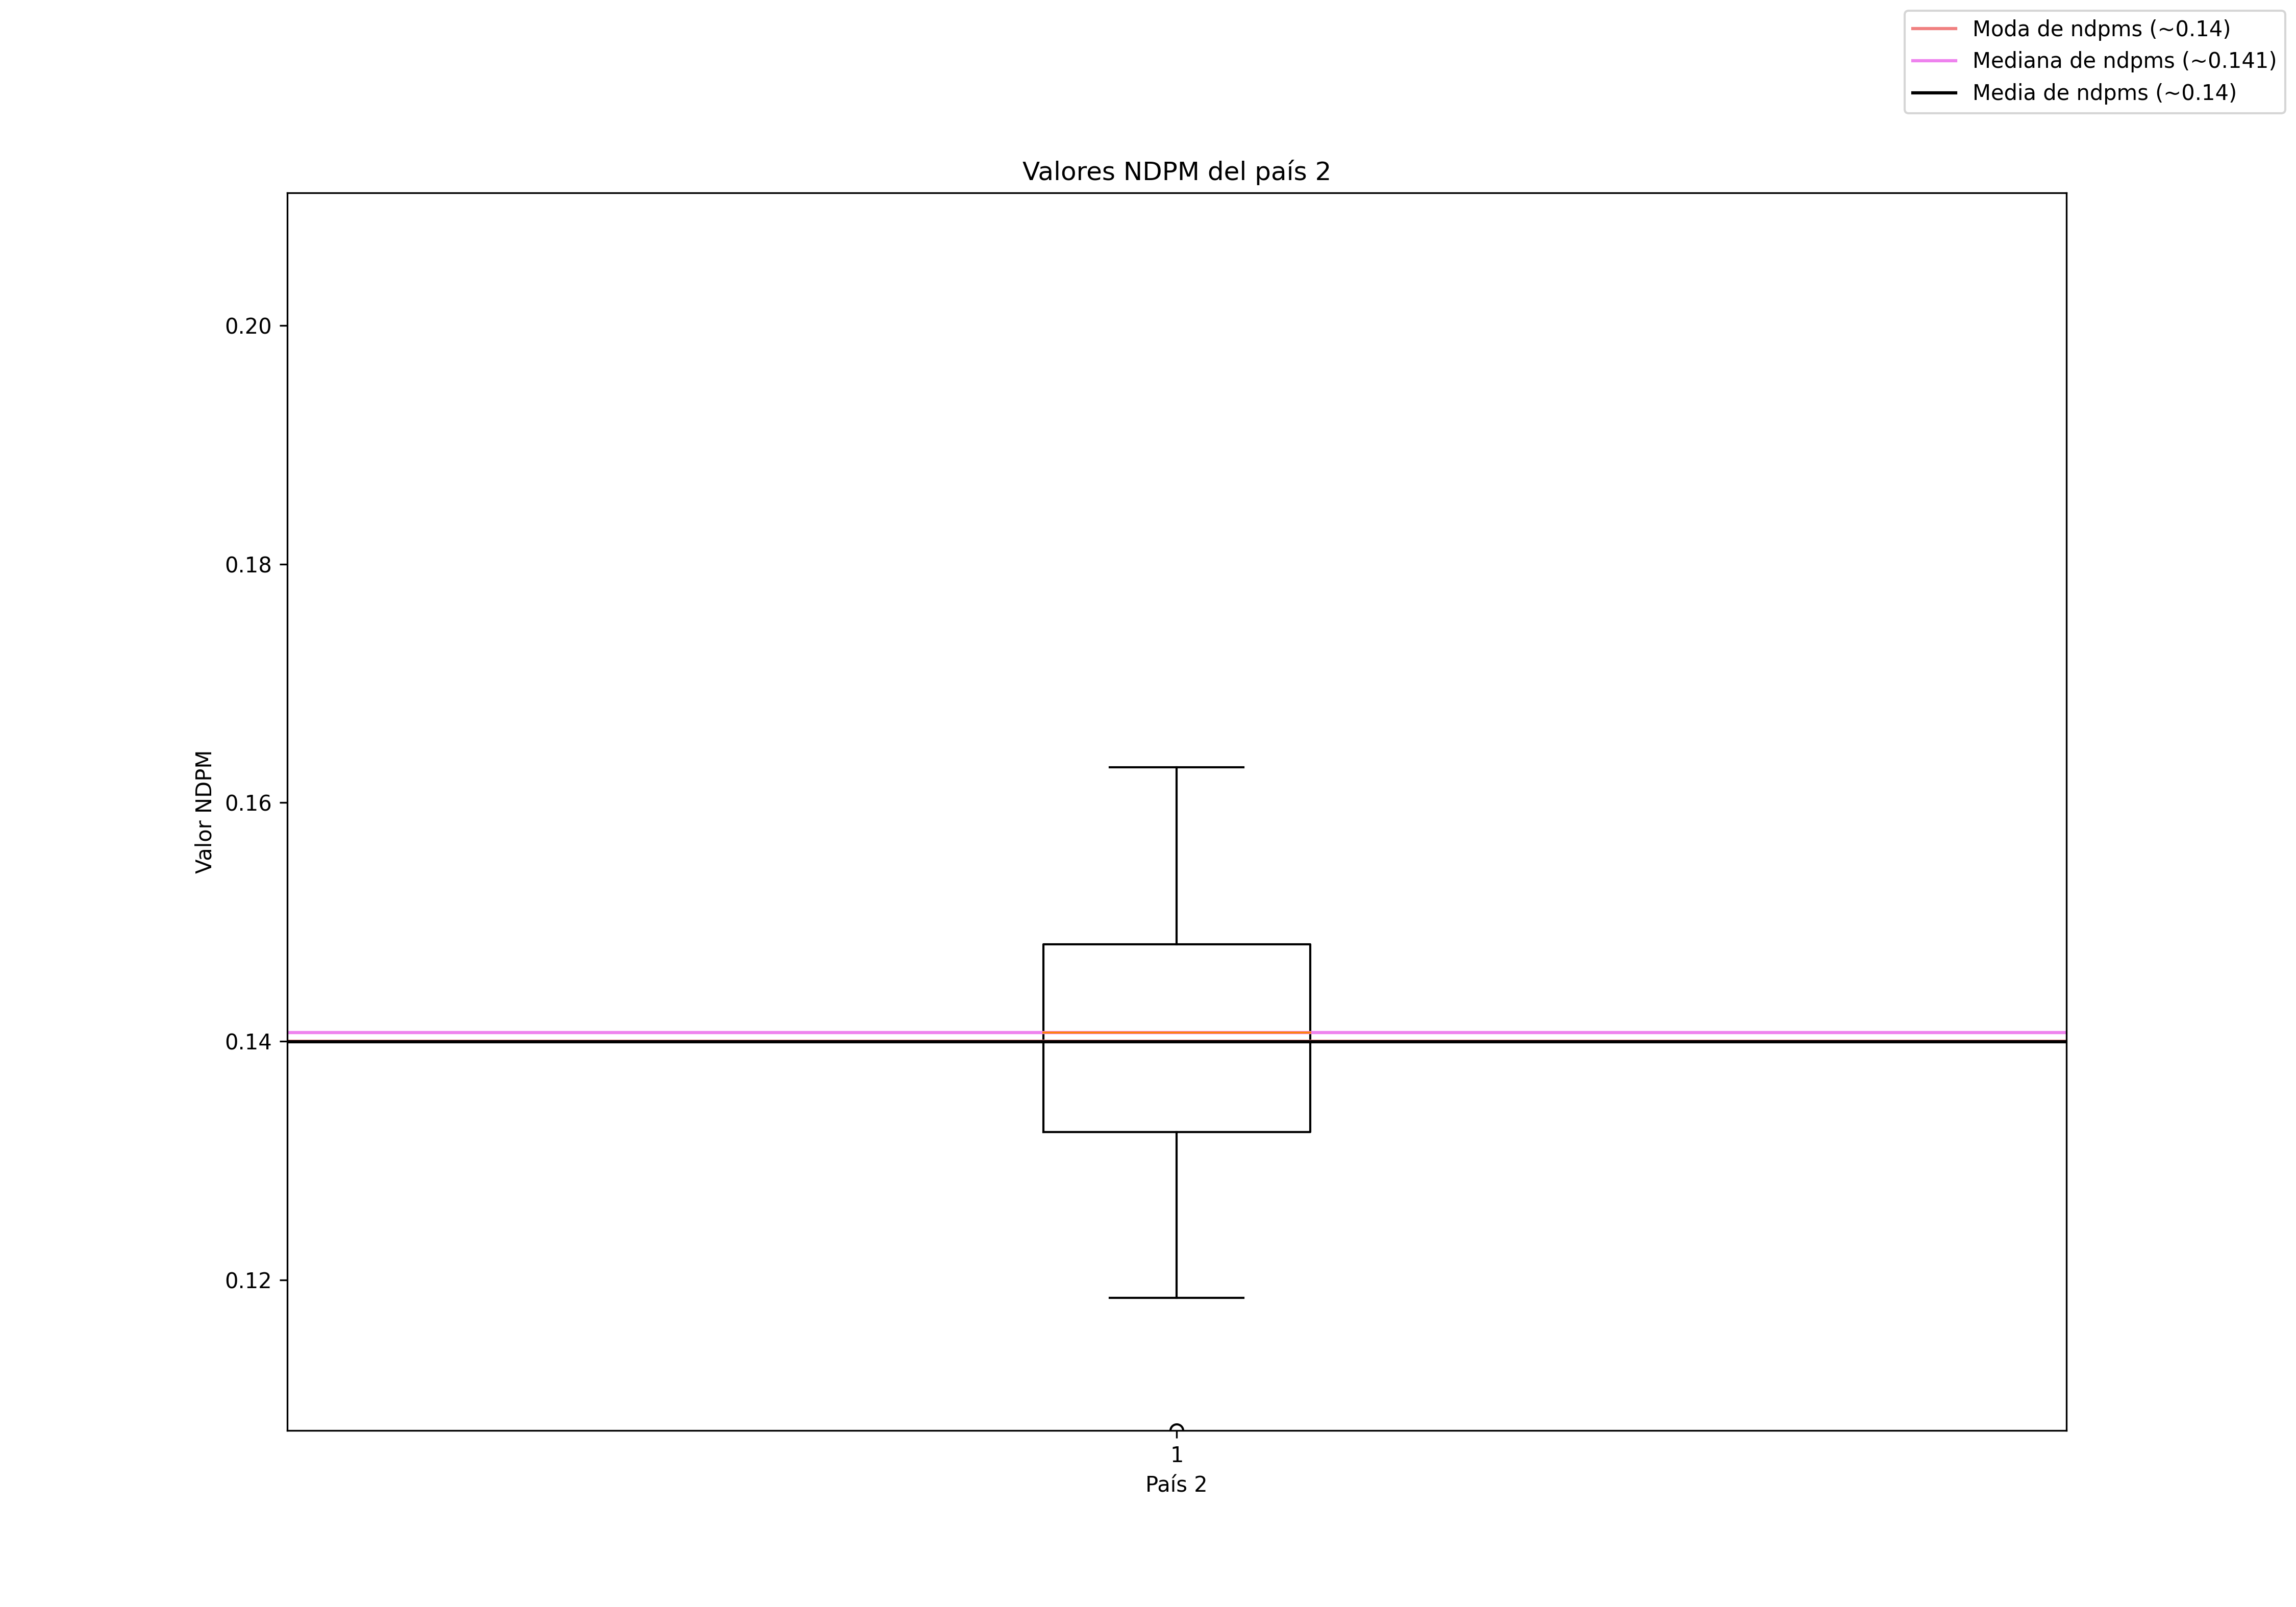
\includegraphics[width=0.5\textheight]
        {Figuras/Reports/PI_2_W1_EXT_CAJAS.png}}
    \caption{Diagramas de cajas y bigotes de los valores NDPM del participante 2\label{fig:PI2_CAJAS}}
\end{sidewaysfigure}
\clearpage
\begin{sidewaysfigure}
    \centering
    \subfloat[Modelo original]
        {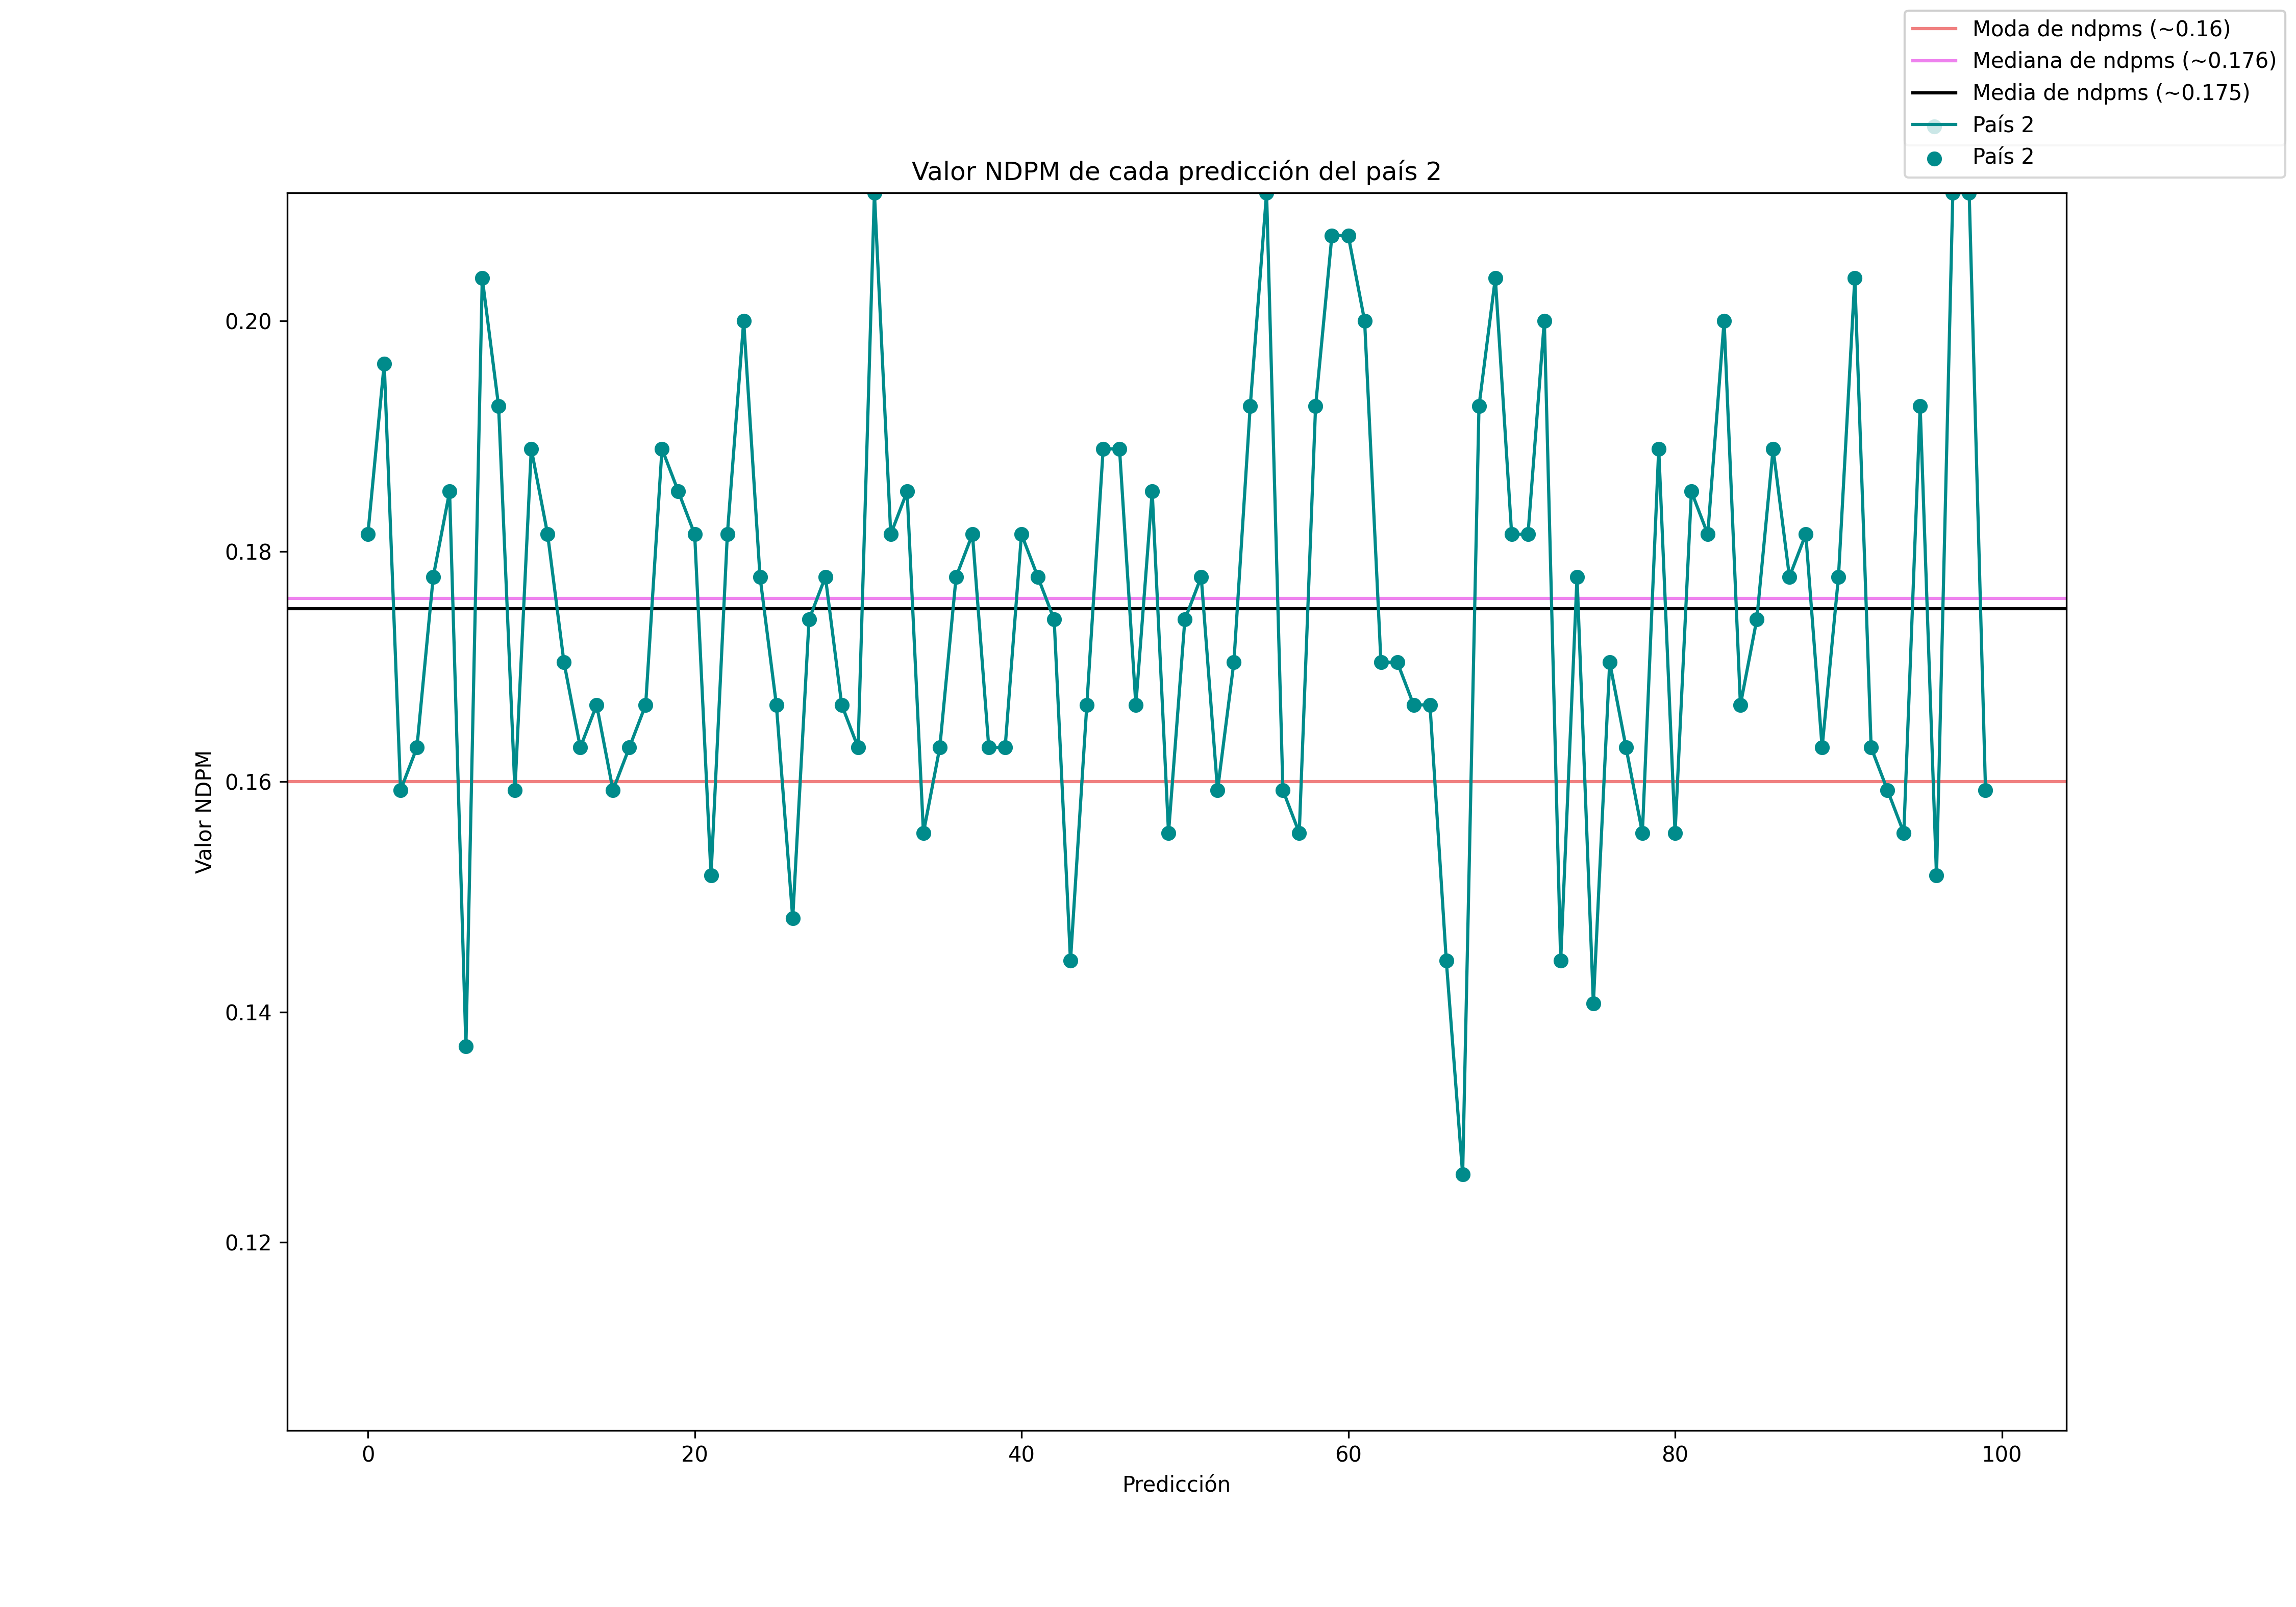
\includegraphics[width=0.5\textheight]
        {Figuras/Reports/PI_2_W0_LOC_DISP.png}}
        \quad
    \subfloat[Reentrenado con \textit{W$_c$ $=0$}]
        {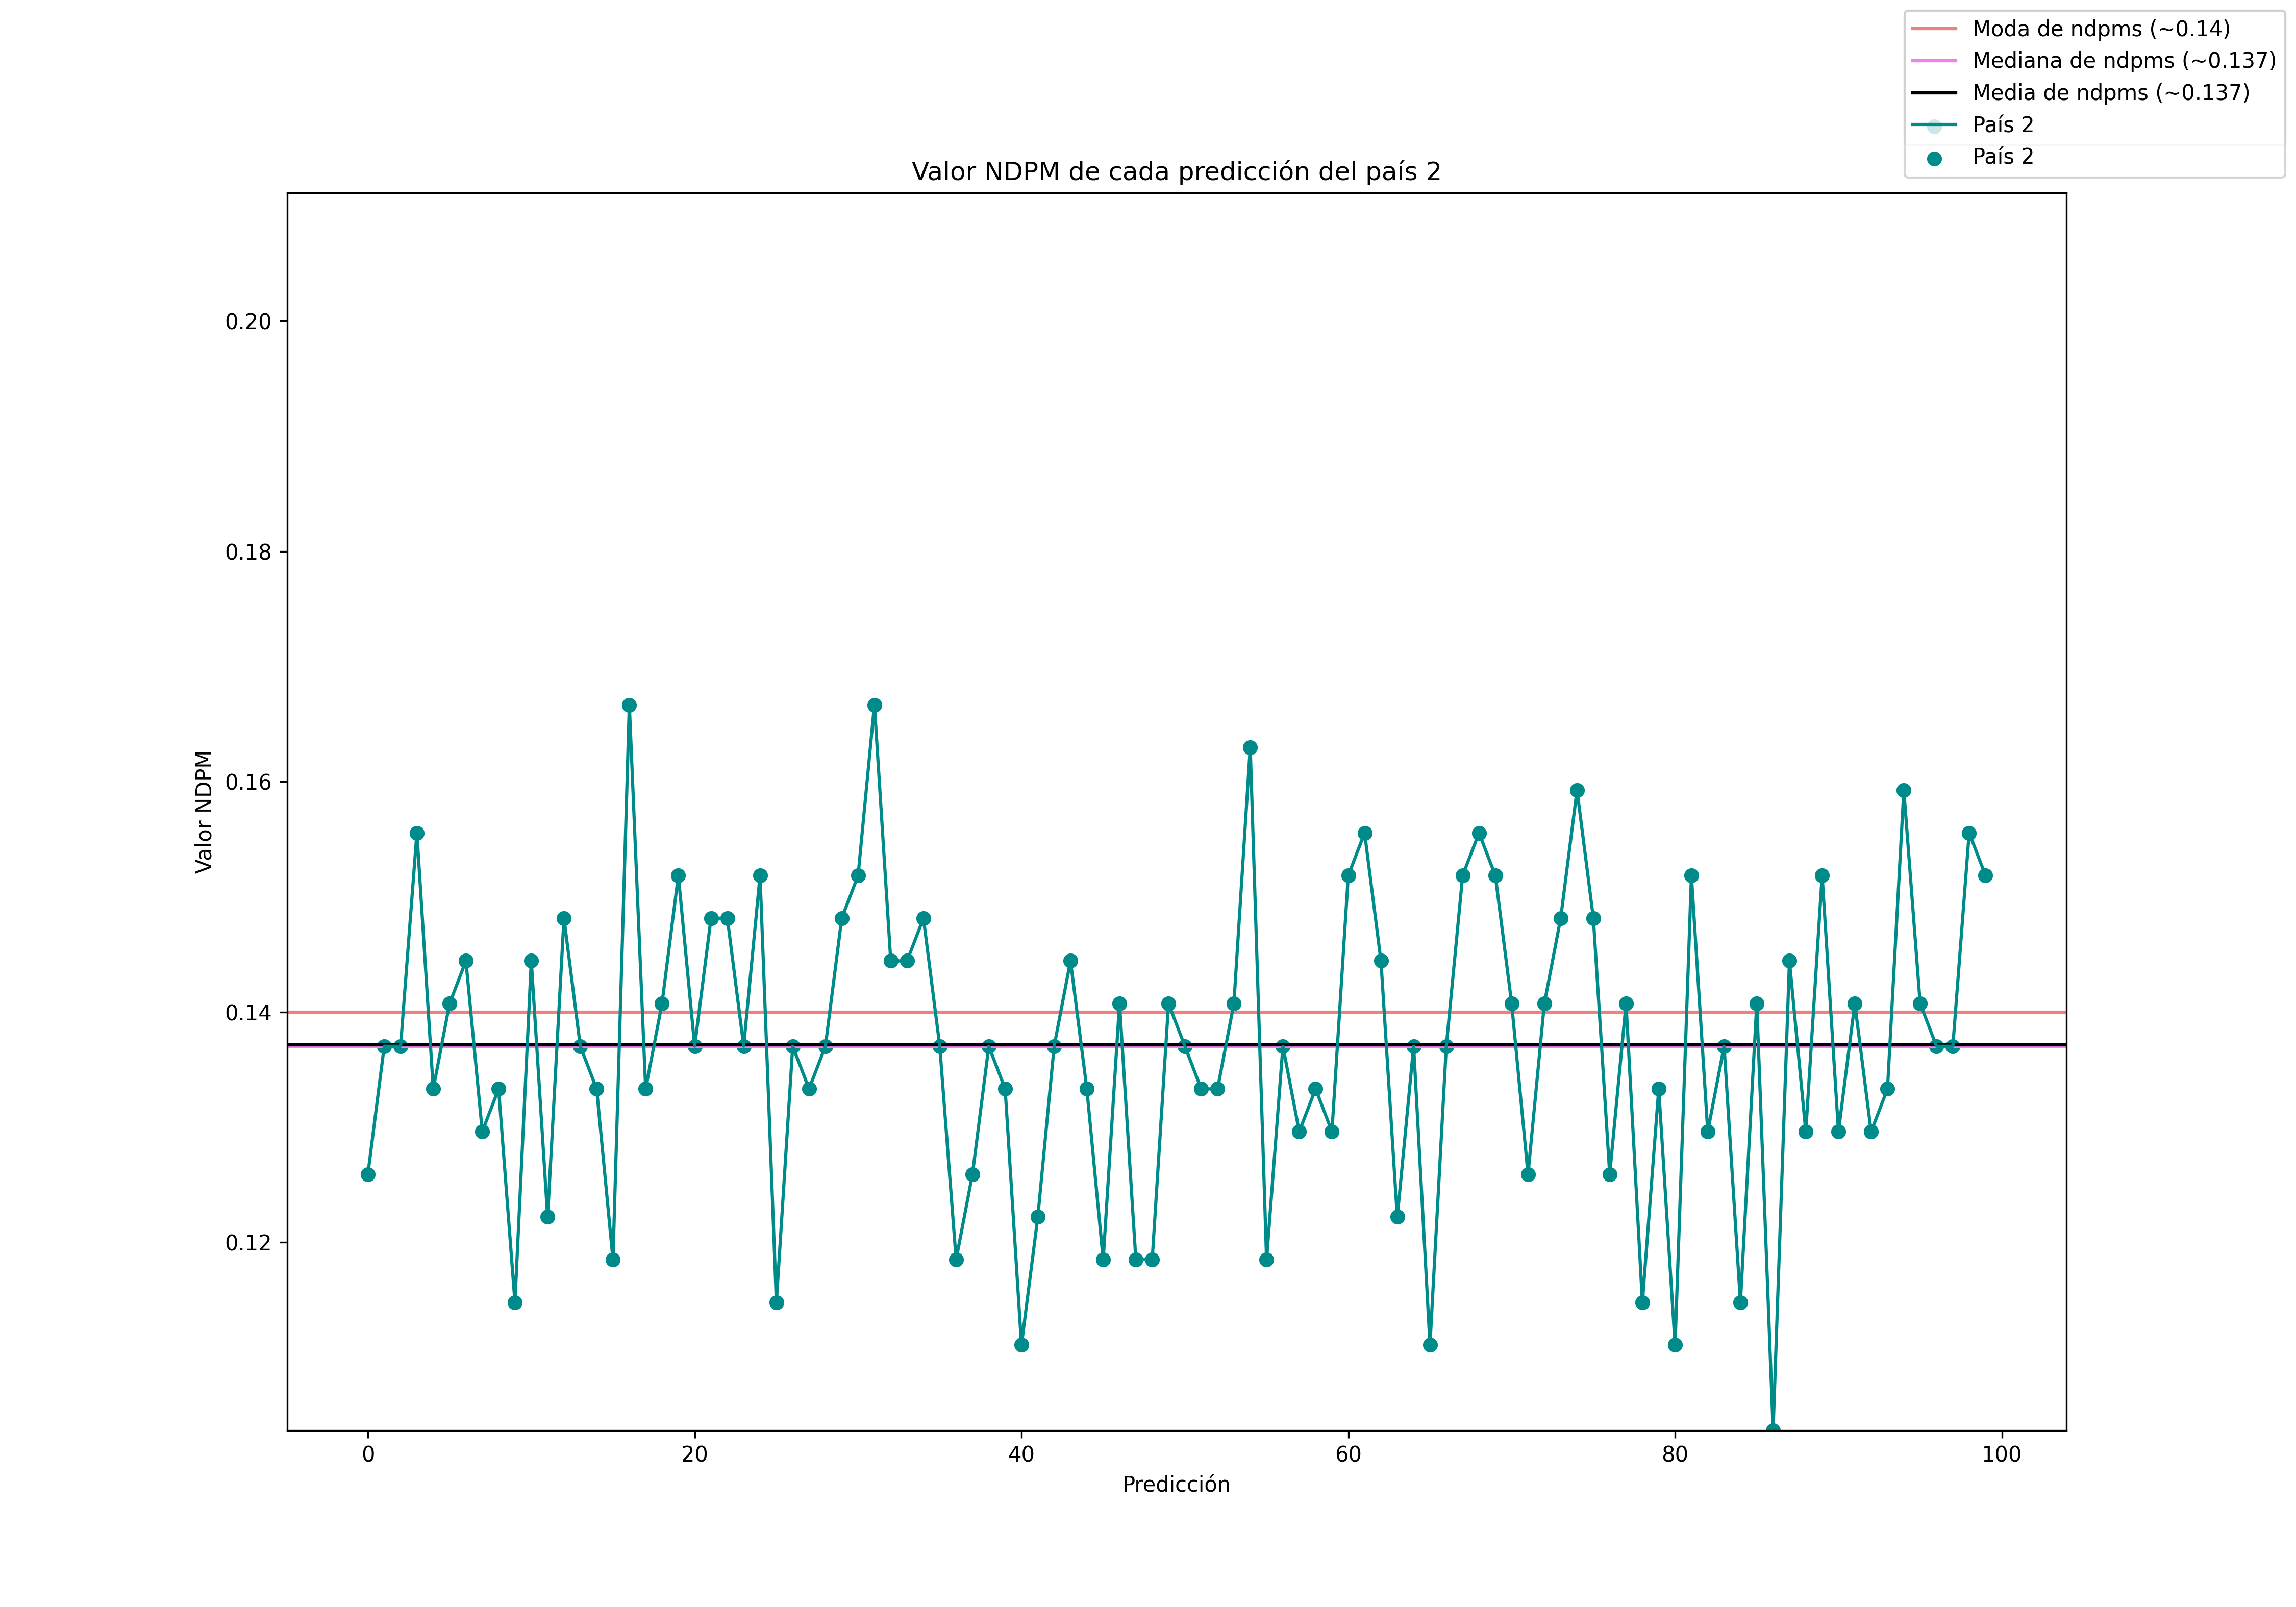
\includegraphics[width=0.5\textheight]
        {Figuras/Reports/PI_2_W0_EXT_DISP.png}}
    \subfloat[Reentrenado con \textit{W$_c$ $=1$}]{
        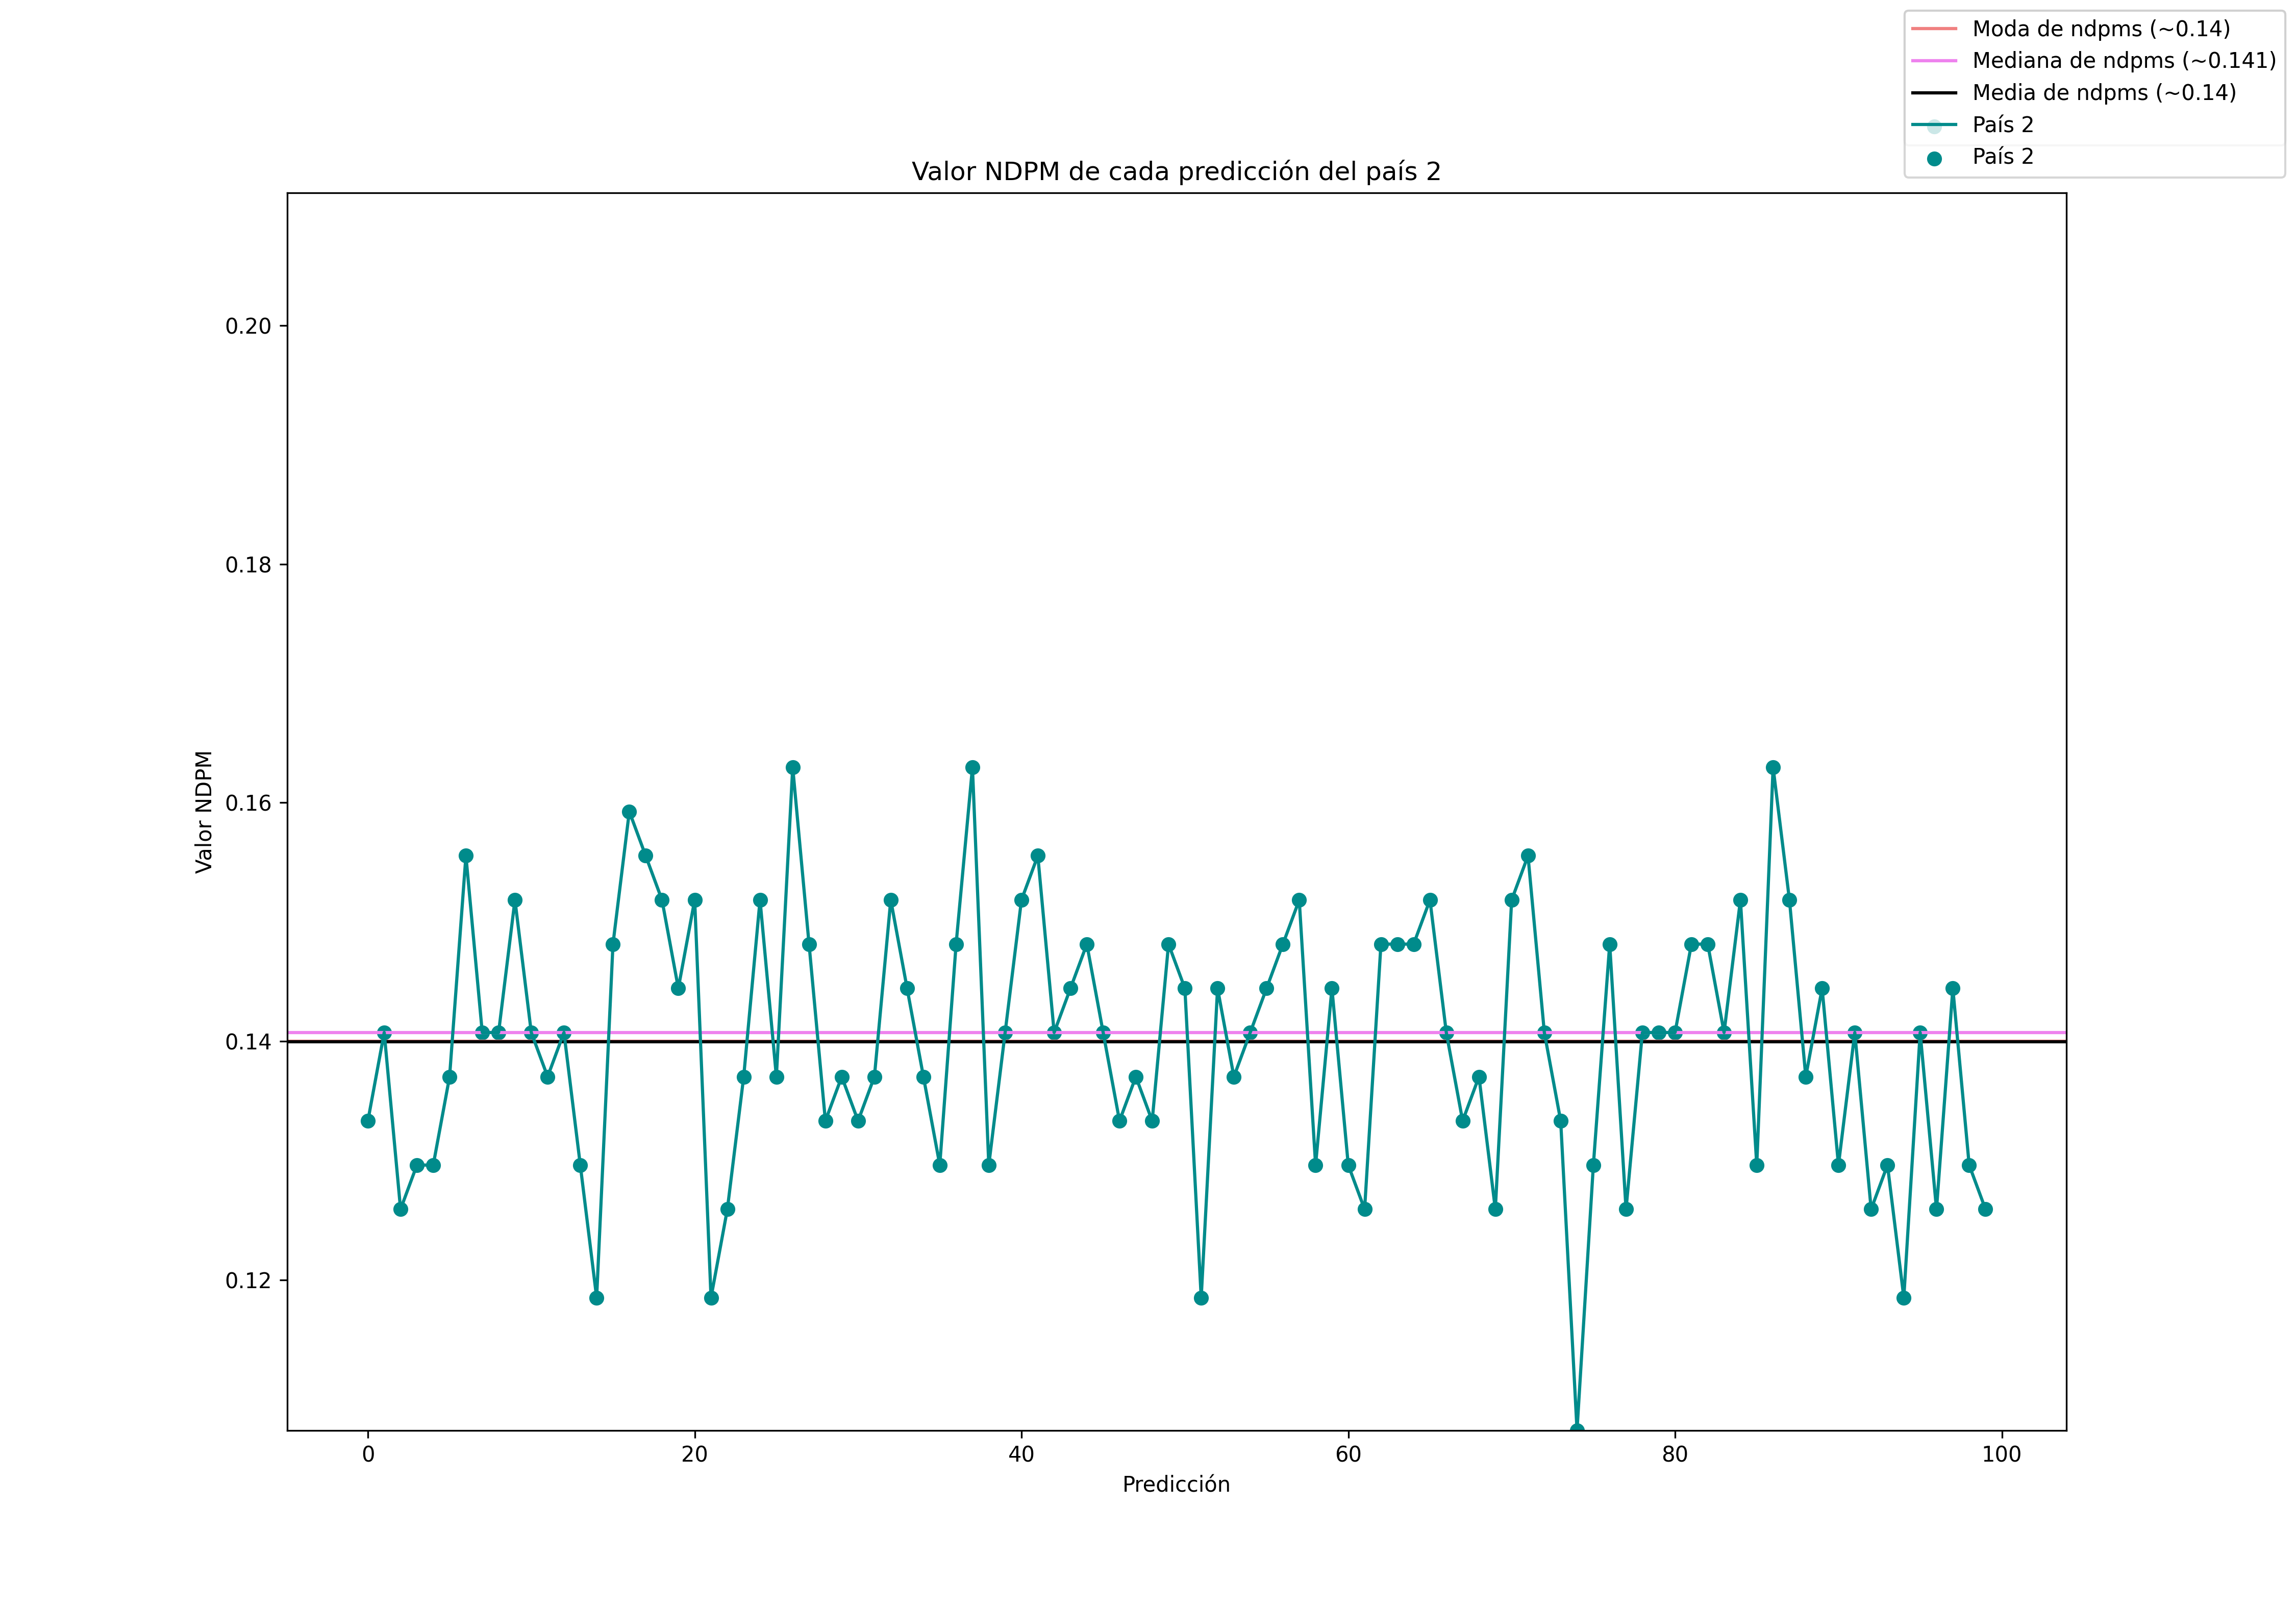
\includegraphics[width=0.5\textheight]
        {Figuras/Reports/PI_2_W1_EXT_DISP.png}}
    \caption{Gráfico de los valores NDPM del participante 2\label{fig:PI2_DISP}}
\end{sidewaysfigure}
\clearpage

\paragraph{Detalle de los resultados del participante 3}
Como se puede observar en los gráficos \ref{fig:PI3_CAJAS} y \ref{fig:PI3_DISP}, los valores del modelo original del participante 3 siempre se mantienen parecidos a los del modelo reentrenado en el servidor de FL, con \textit{W$_c$ $=1$} el valor del modelo reentrenado es peor que el original pero con \textit{W$_c$ $=0$} el valor del modelo reentrenado es mejor que el original. En los gráficos se pueden observar varias líneas horizontales que hacen referencia a la media, mediana y moda, dibujadas en negro, rosa y marrón respectivamente.

\paragraph{Detalle de los resultados del participante 4}
Como se puede observar en los gráficos \ref{fig:PI4_CAJAS} y \ref{fig:PI4_DISP}, los valores del modelo original del participante 4 siempre se mantienen por debajo de los del modelo reentrenado en el servidor de FL, tanto con \textit{W$_c$ $=1$} como con \textit{W$_c$ $=0$}, aunque no con tanta diferencia como el participante 2. En los gráficos se pueden observar varias líneas horizontales que hacen referencia a la media, mediana y moda, dibujadas en negro, rosa y marrón respectivamente.

\begin{sidewaysfigure}
    \centering
    \subfloat[Modelo original]
        {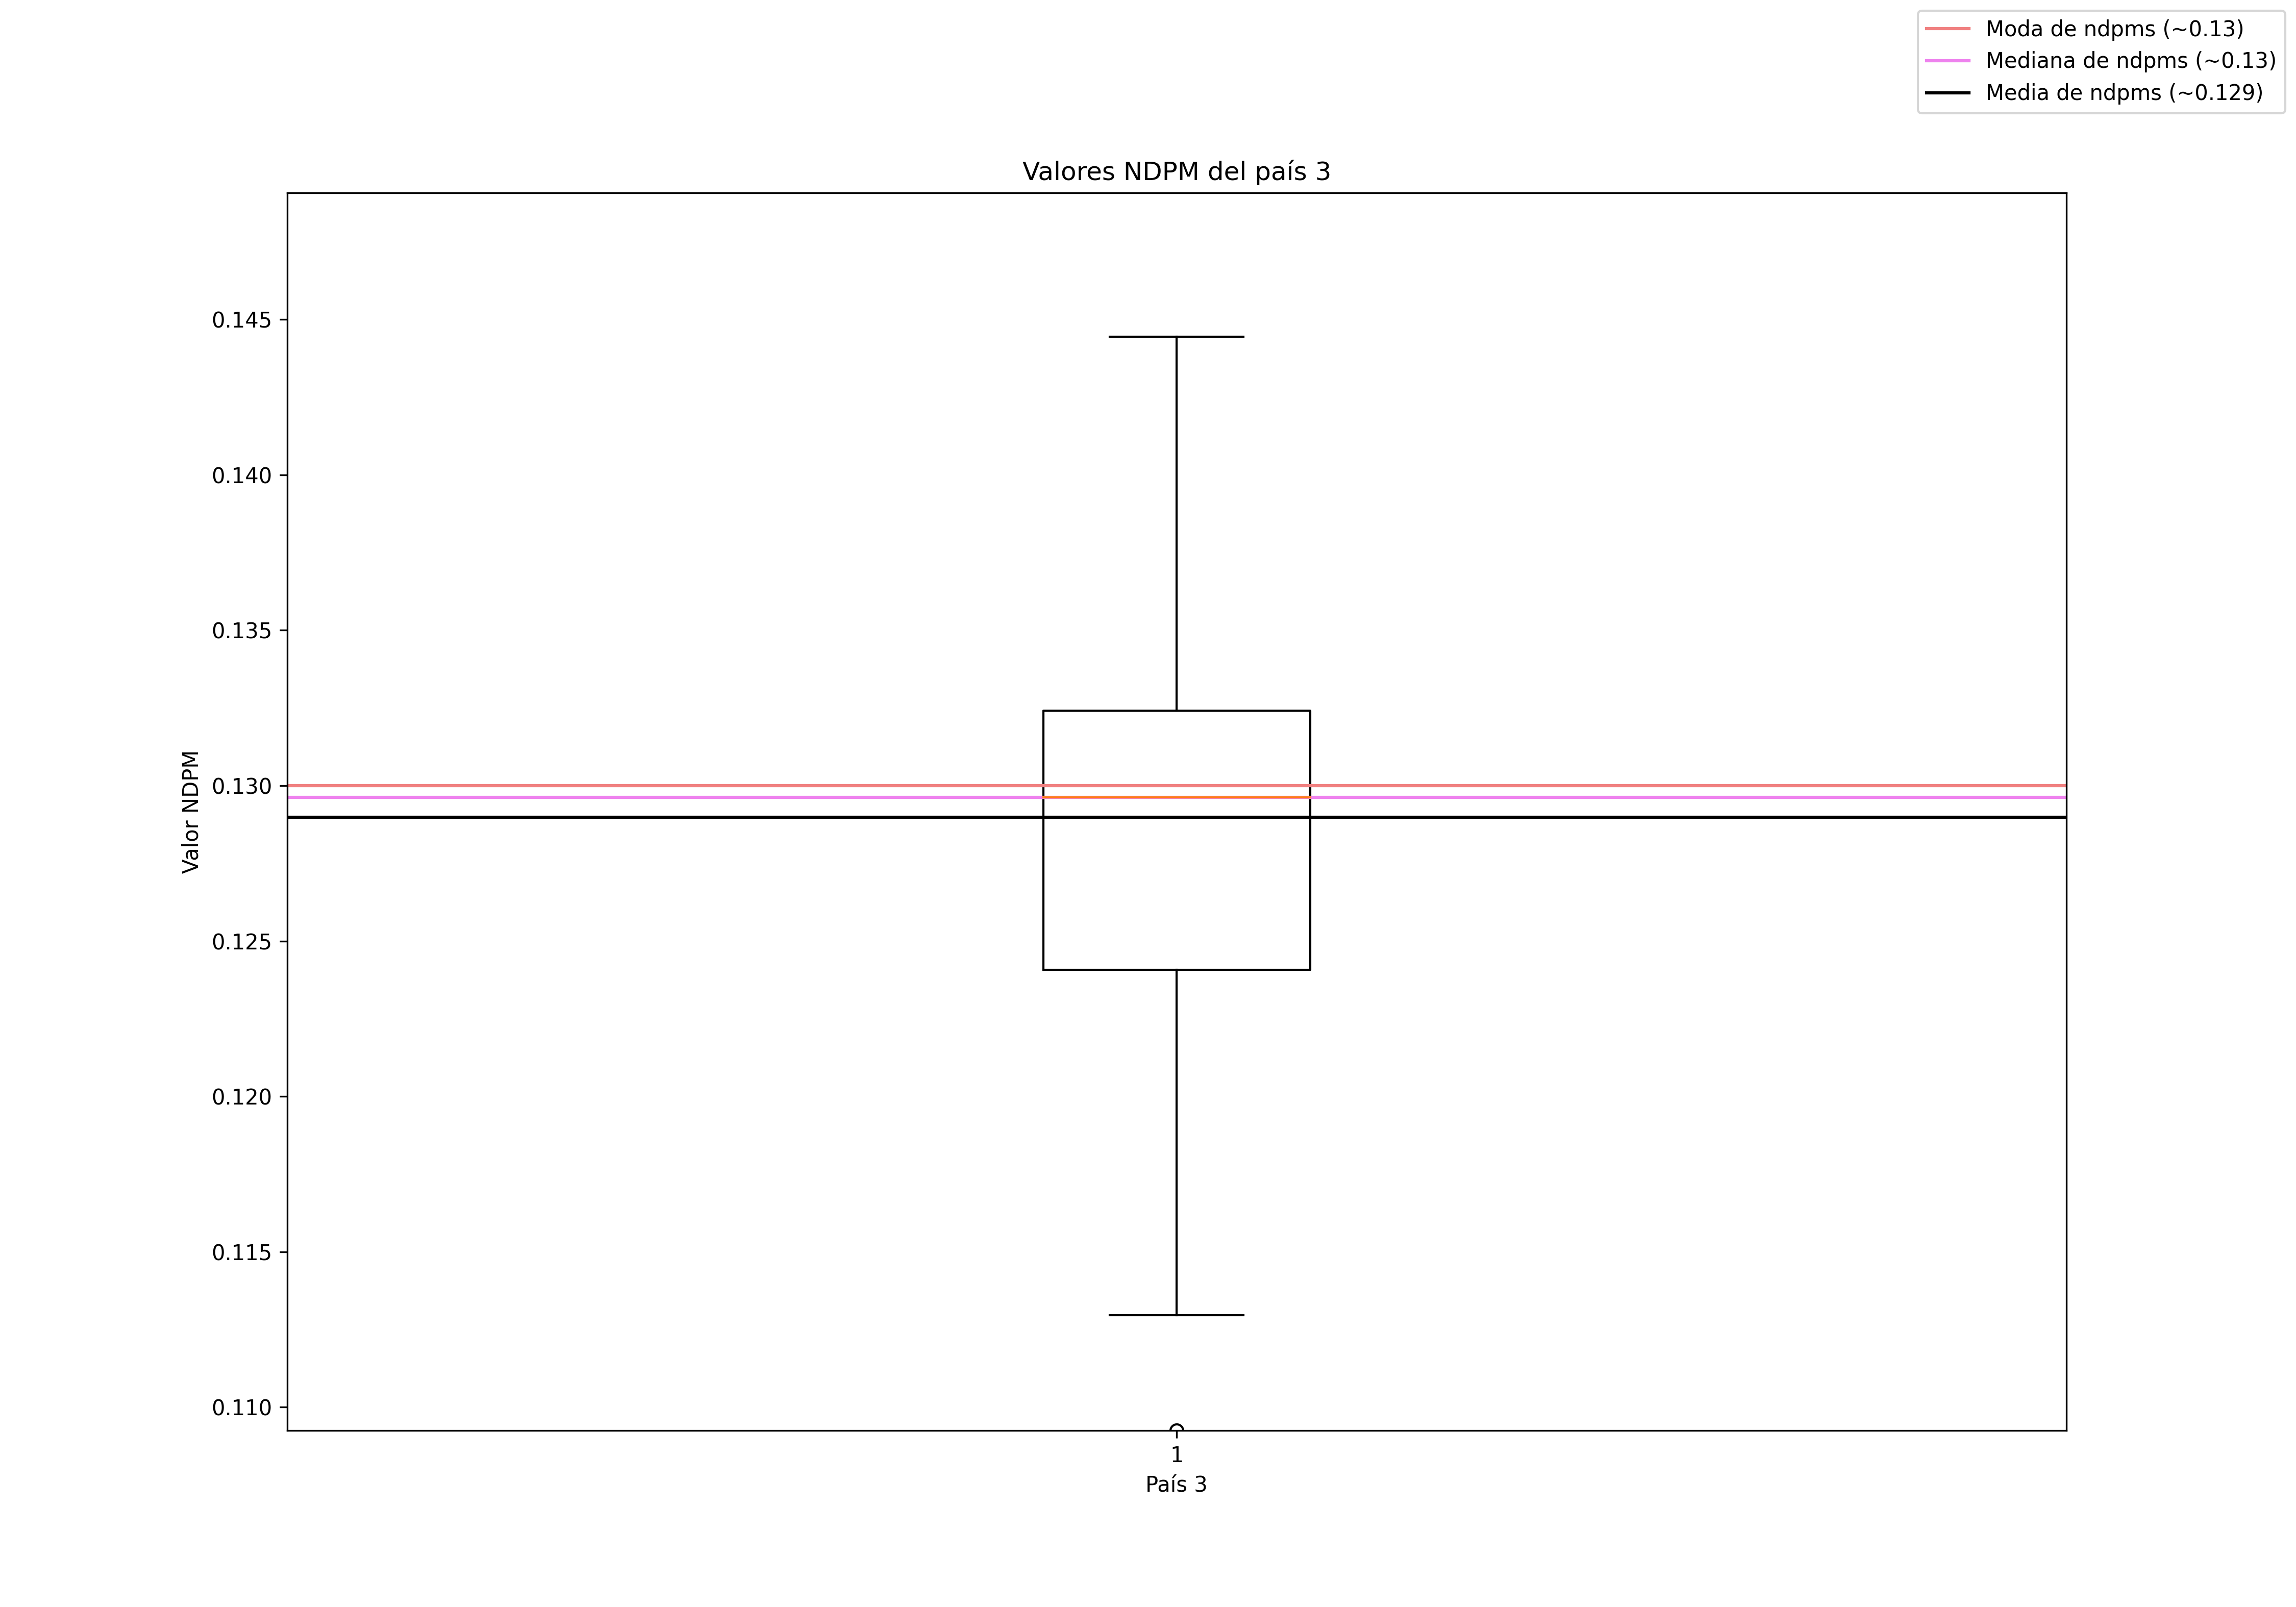
\includegraphics[width=0.5\textheight]
        {Figuras/Reports/PI_3_W0_LOC_CAJAS.png}}
        \quad
    \subfloat[Reentrenado con \textit{W$_c$ $=0$}]
        {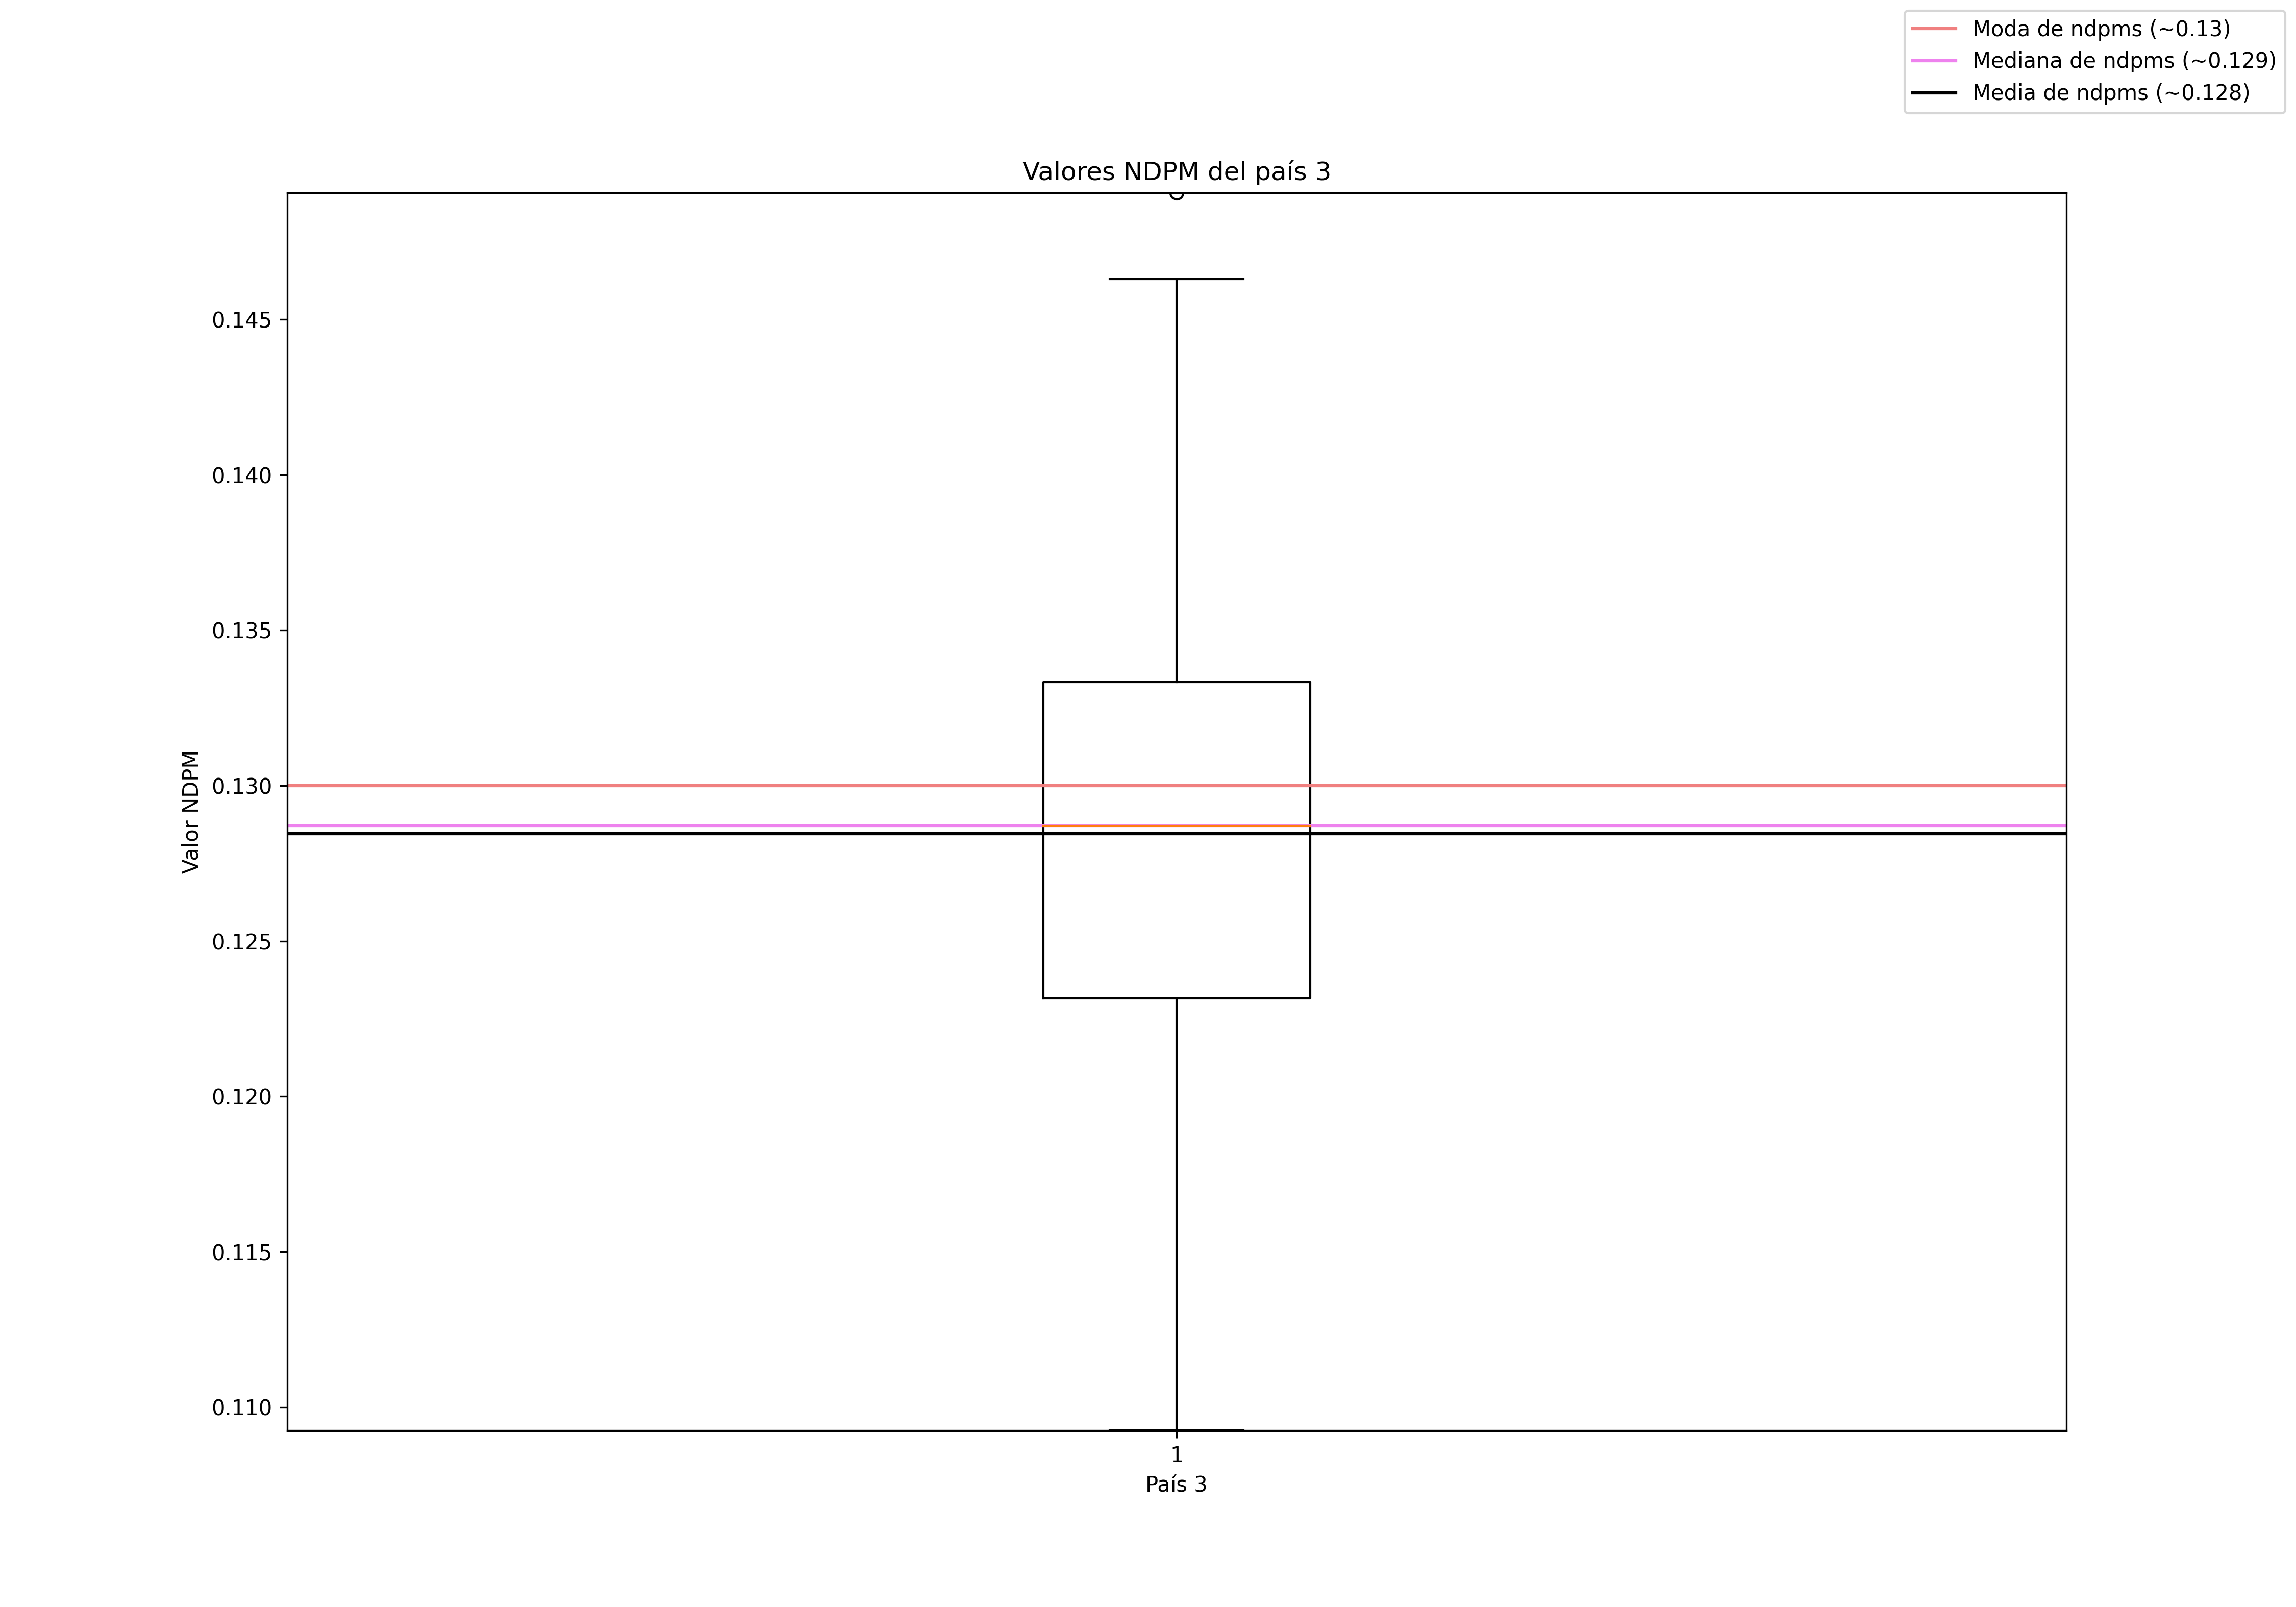
\includegraphics[width=0.5\textheight]
        {Figuras/Reports/PI_3_W0_EXT_CAJAS.png}}
    \subfloat[Reentrenado con \textit{W$_c$ $=1$}]{
        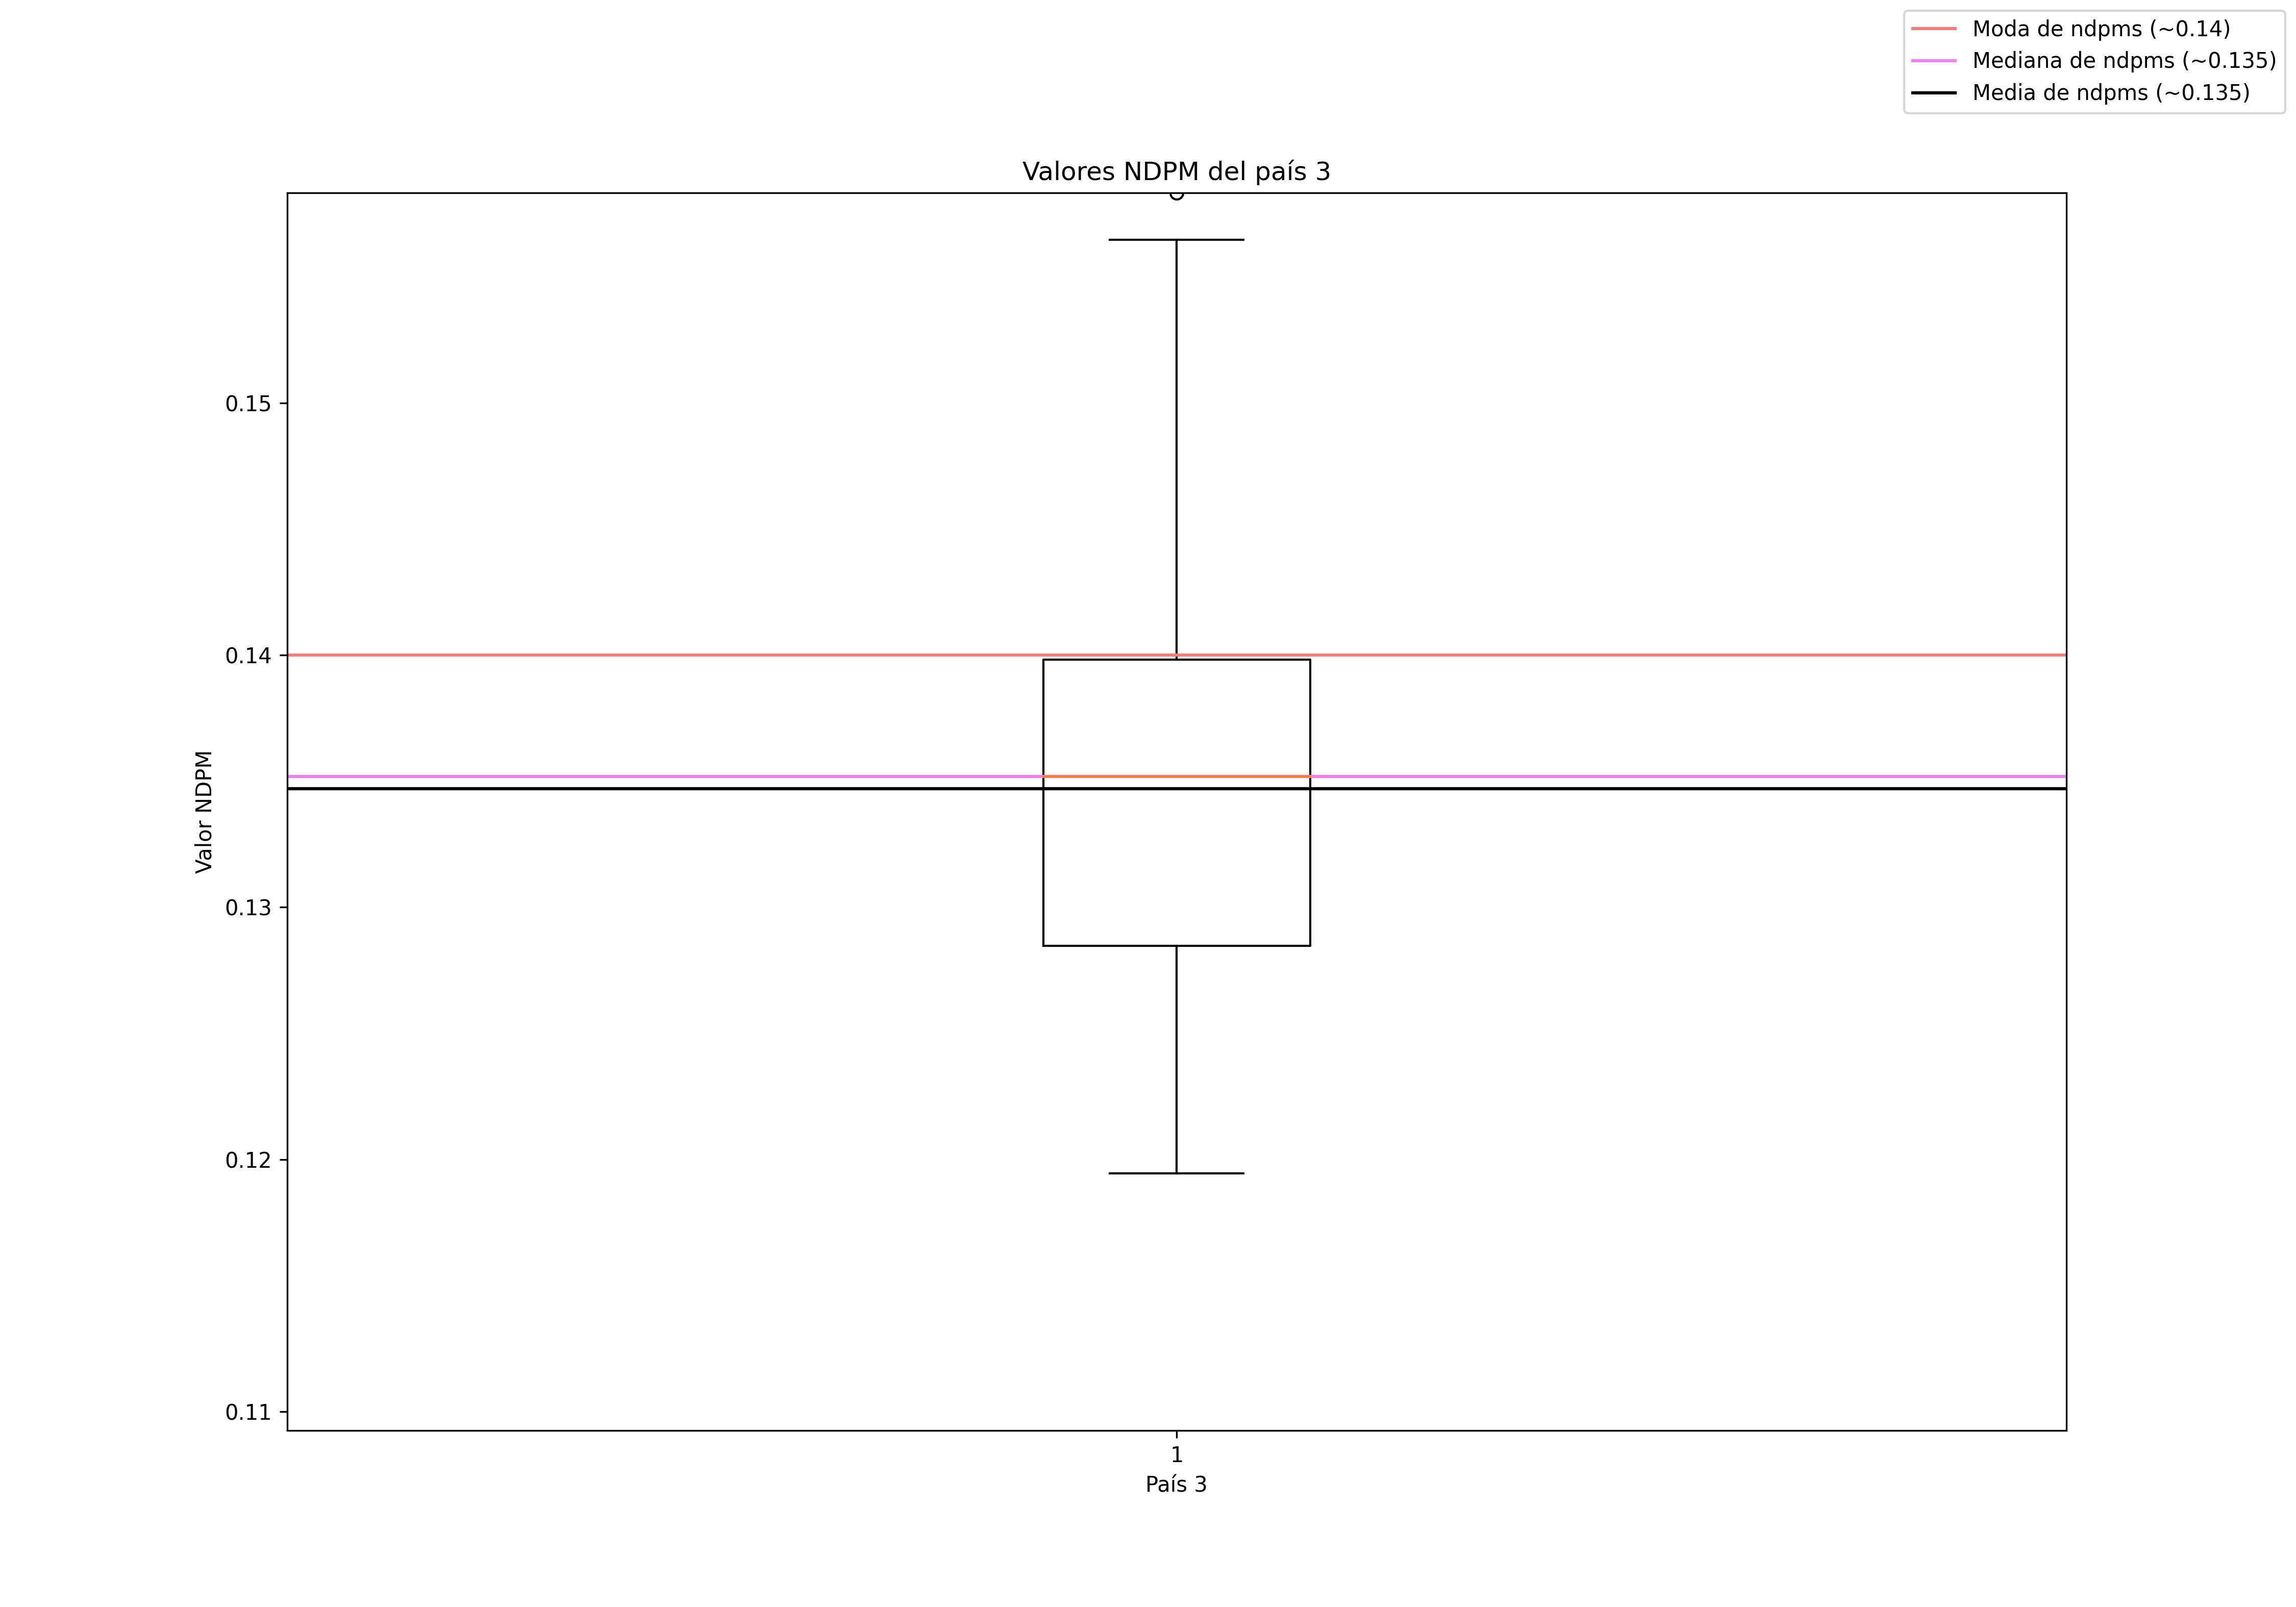
\includegraphics[width=0.5\textheight]
        {Figuras/Reports/PI_3_W1_EXT_CAJAS.png}}
    \caption{Diagramas de cajas y bigotes de los valores NDPM del participante 3\label{fig:PI3_CAJAS}}
\end{sidewaysfigure}
\clearpage
\begin{sidewaysfigure}
    \centering
    \subfloat[Modelo original]
        {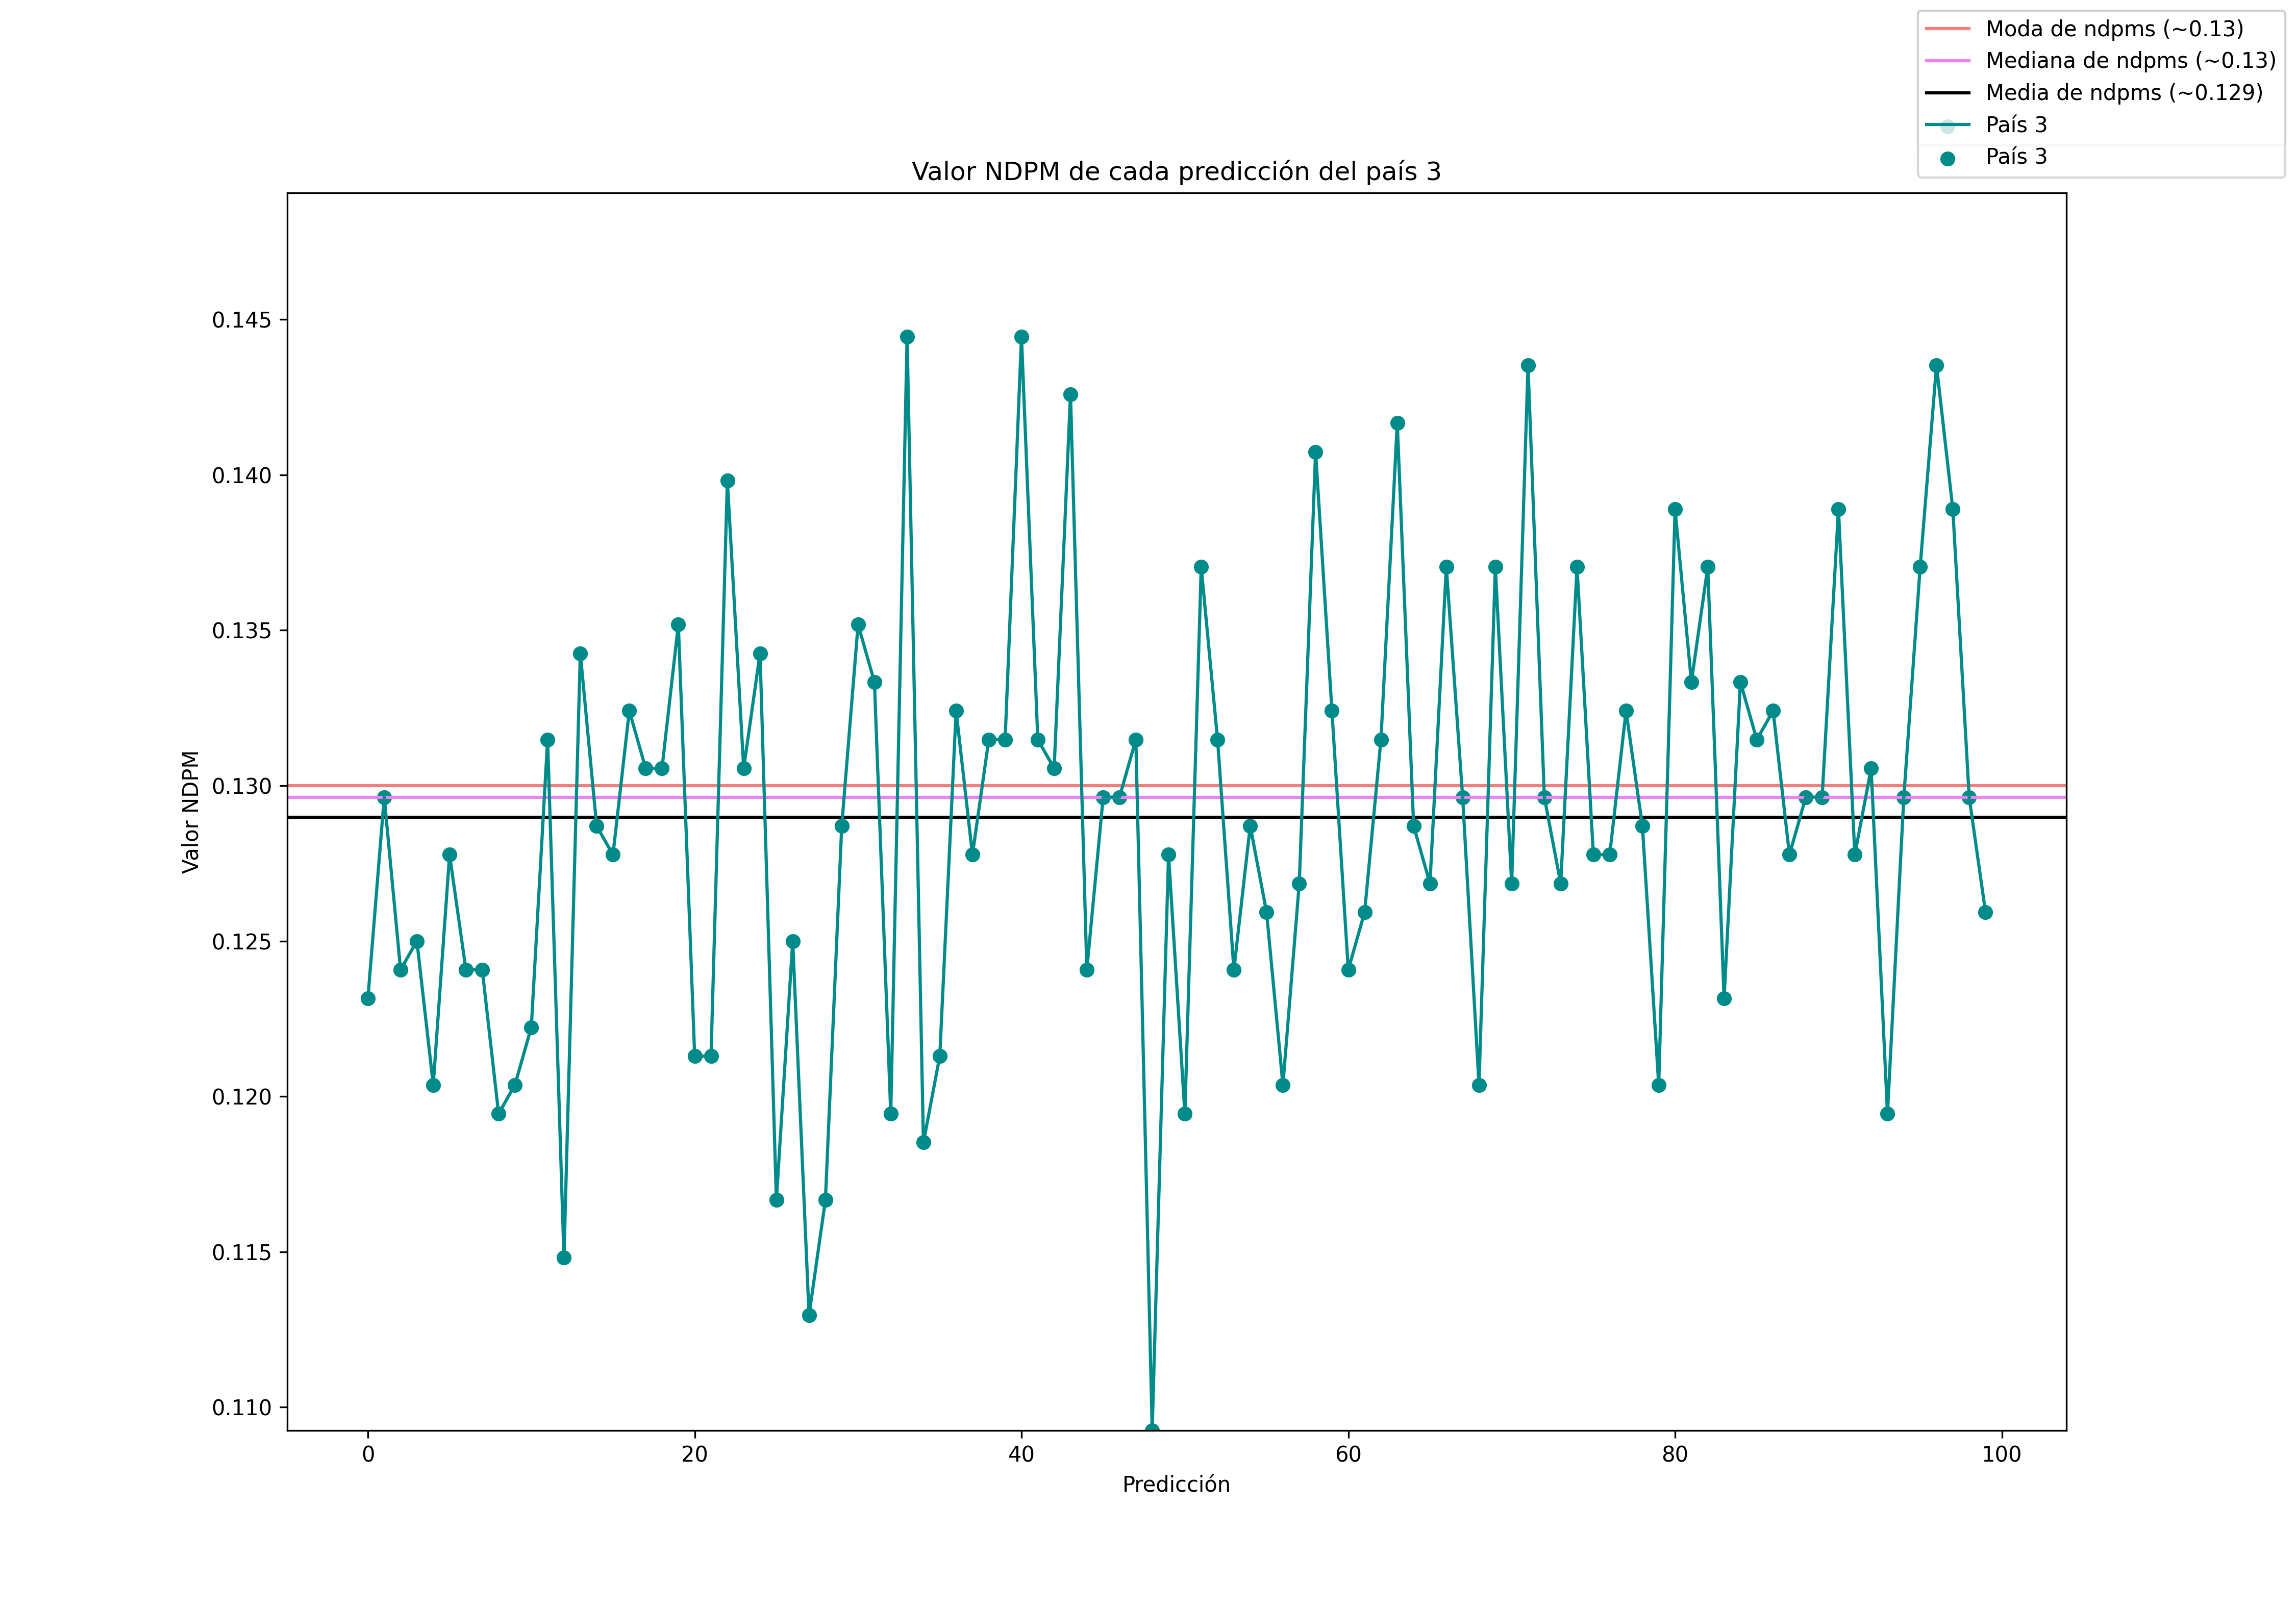
\includegraphics[width=0.5\textheight]
        {Figuras/Reports/PI_3_W0_LOC_DISP.png}}
        \quad
    \subfloat[Reentrenado con \textit{W$_c$ $=0$}]
        {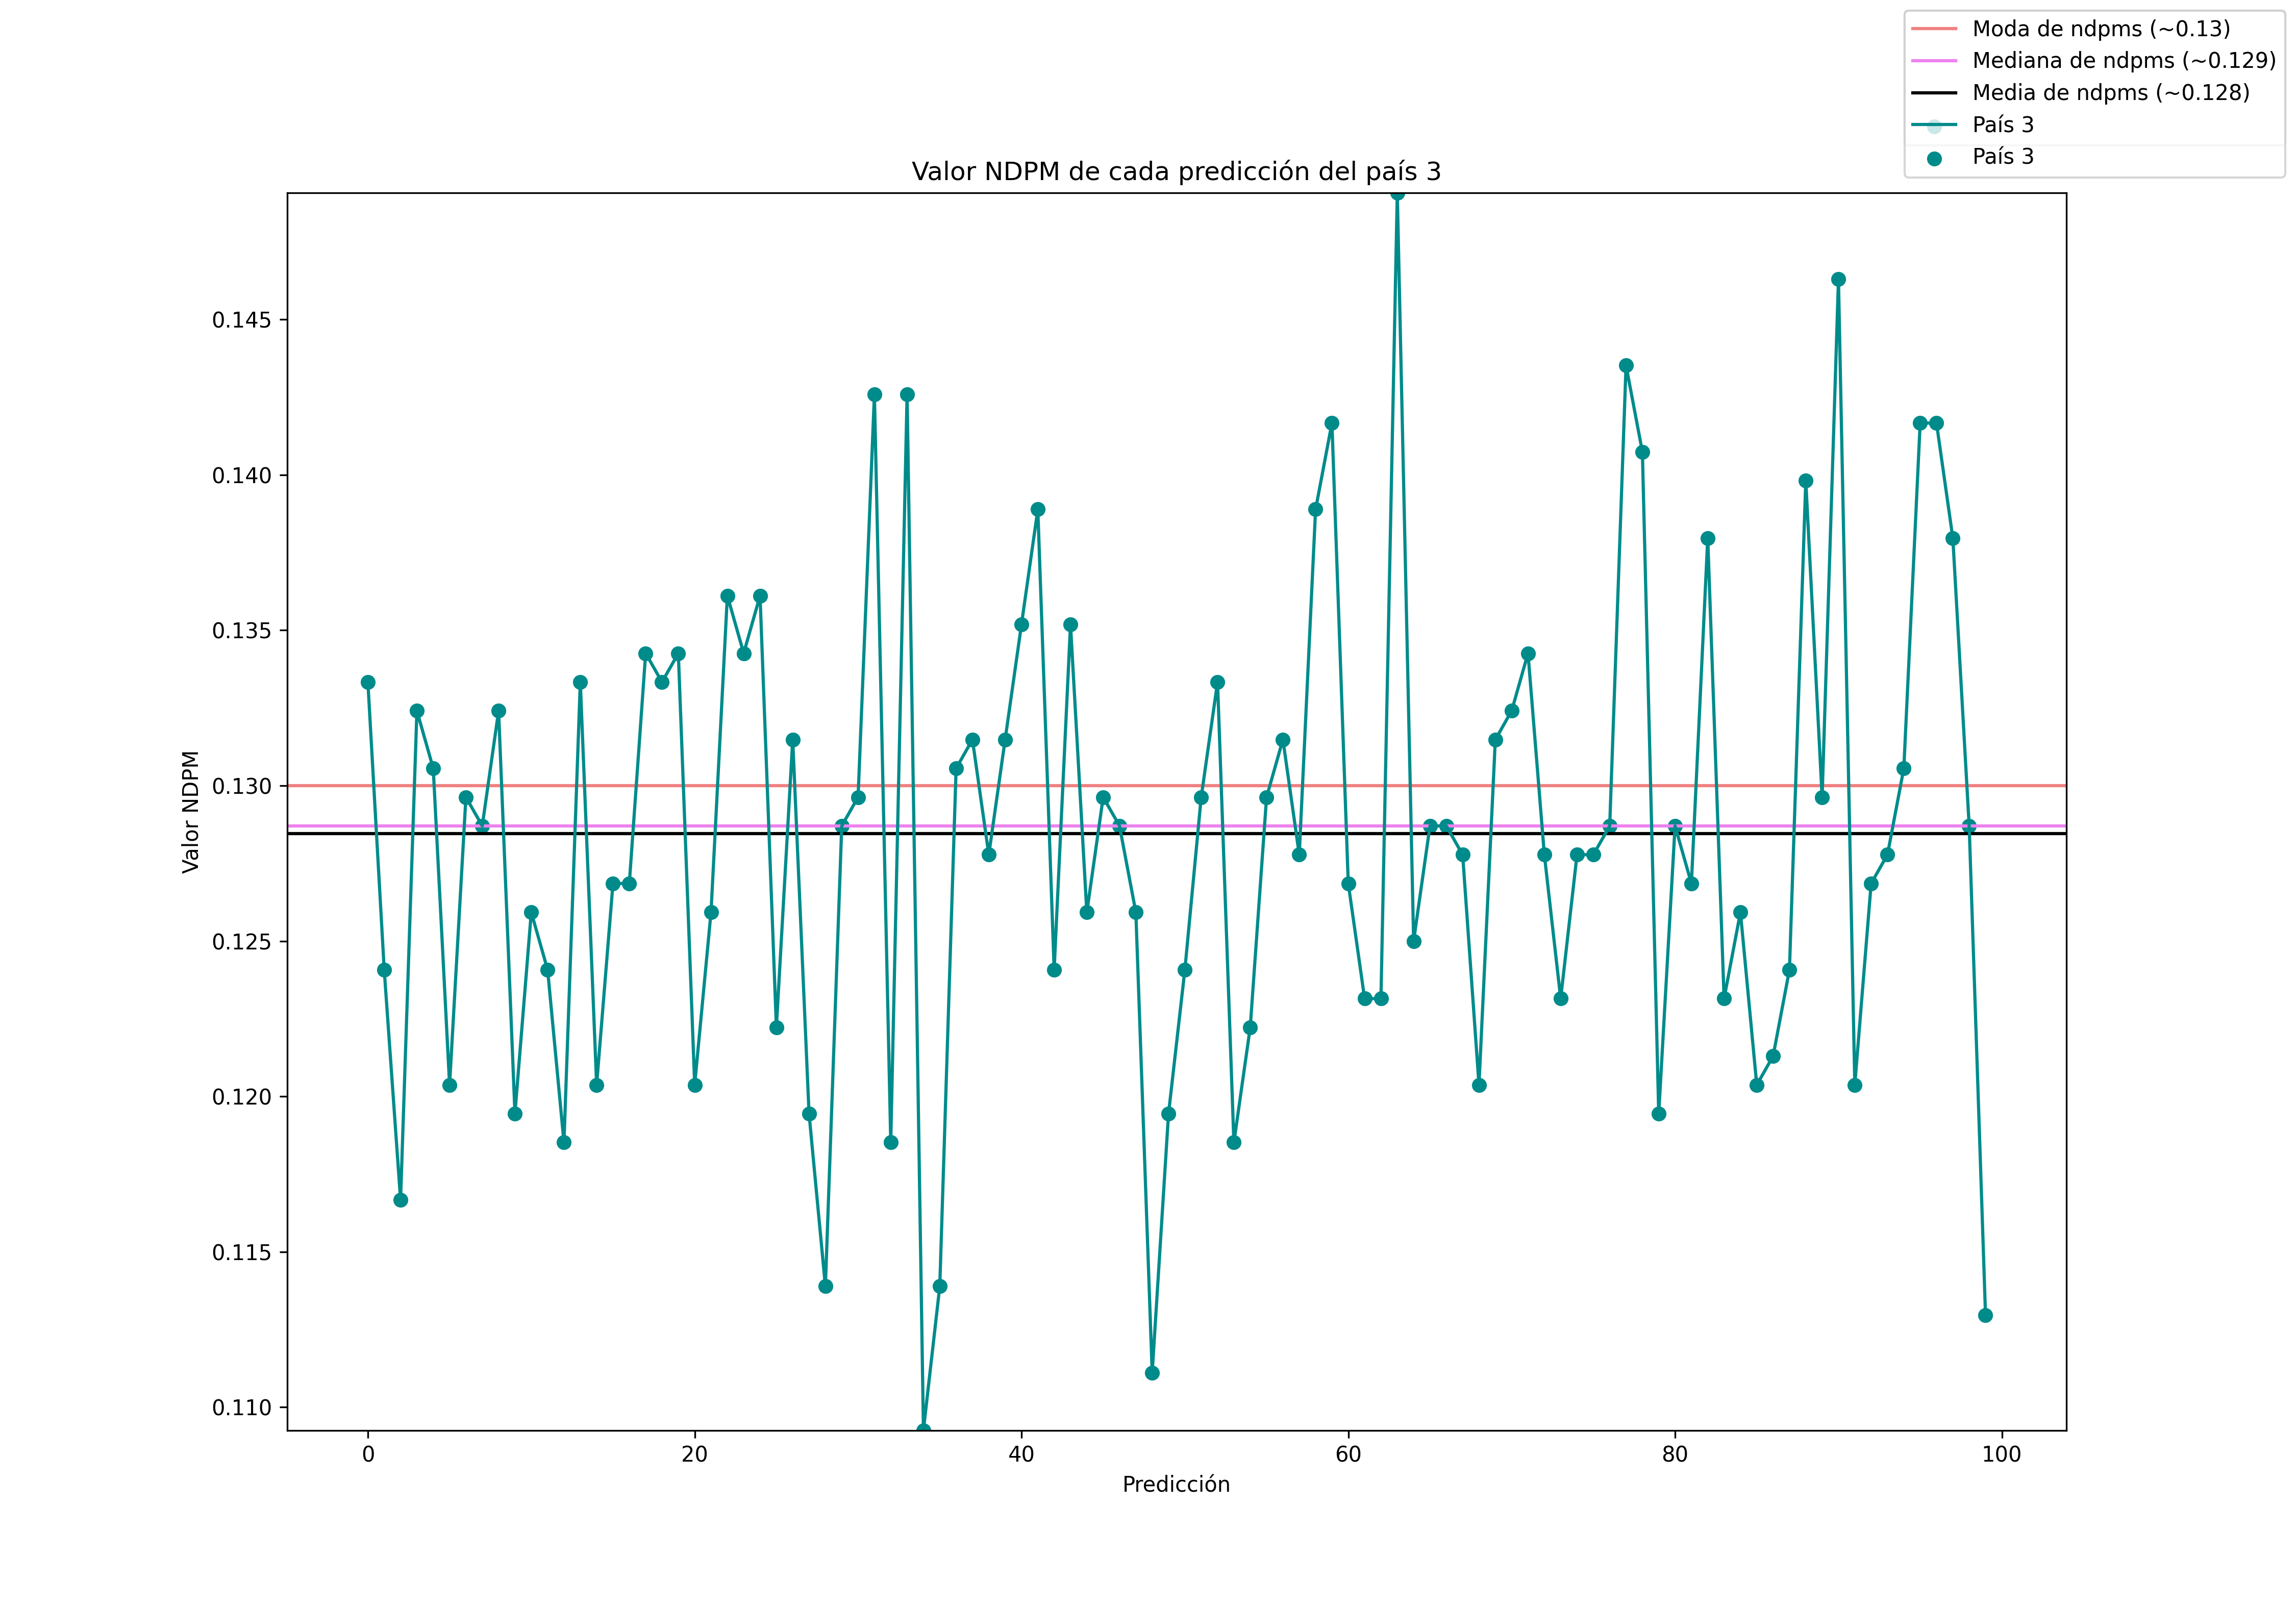
\includegraphics[width=0.5\textheight]
        {Figuras/Reports/PI_3_W0_EXT_DISP.png}}
    \subfloat[Reentrenado con \textit{W$_c$ $=1$}]{
        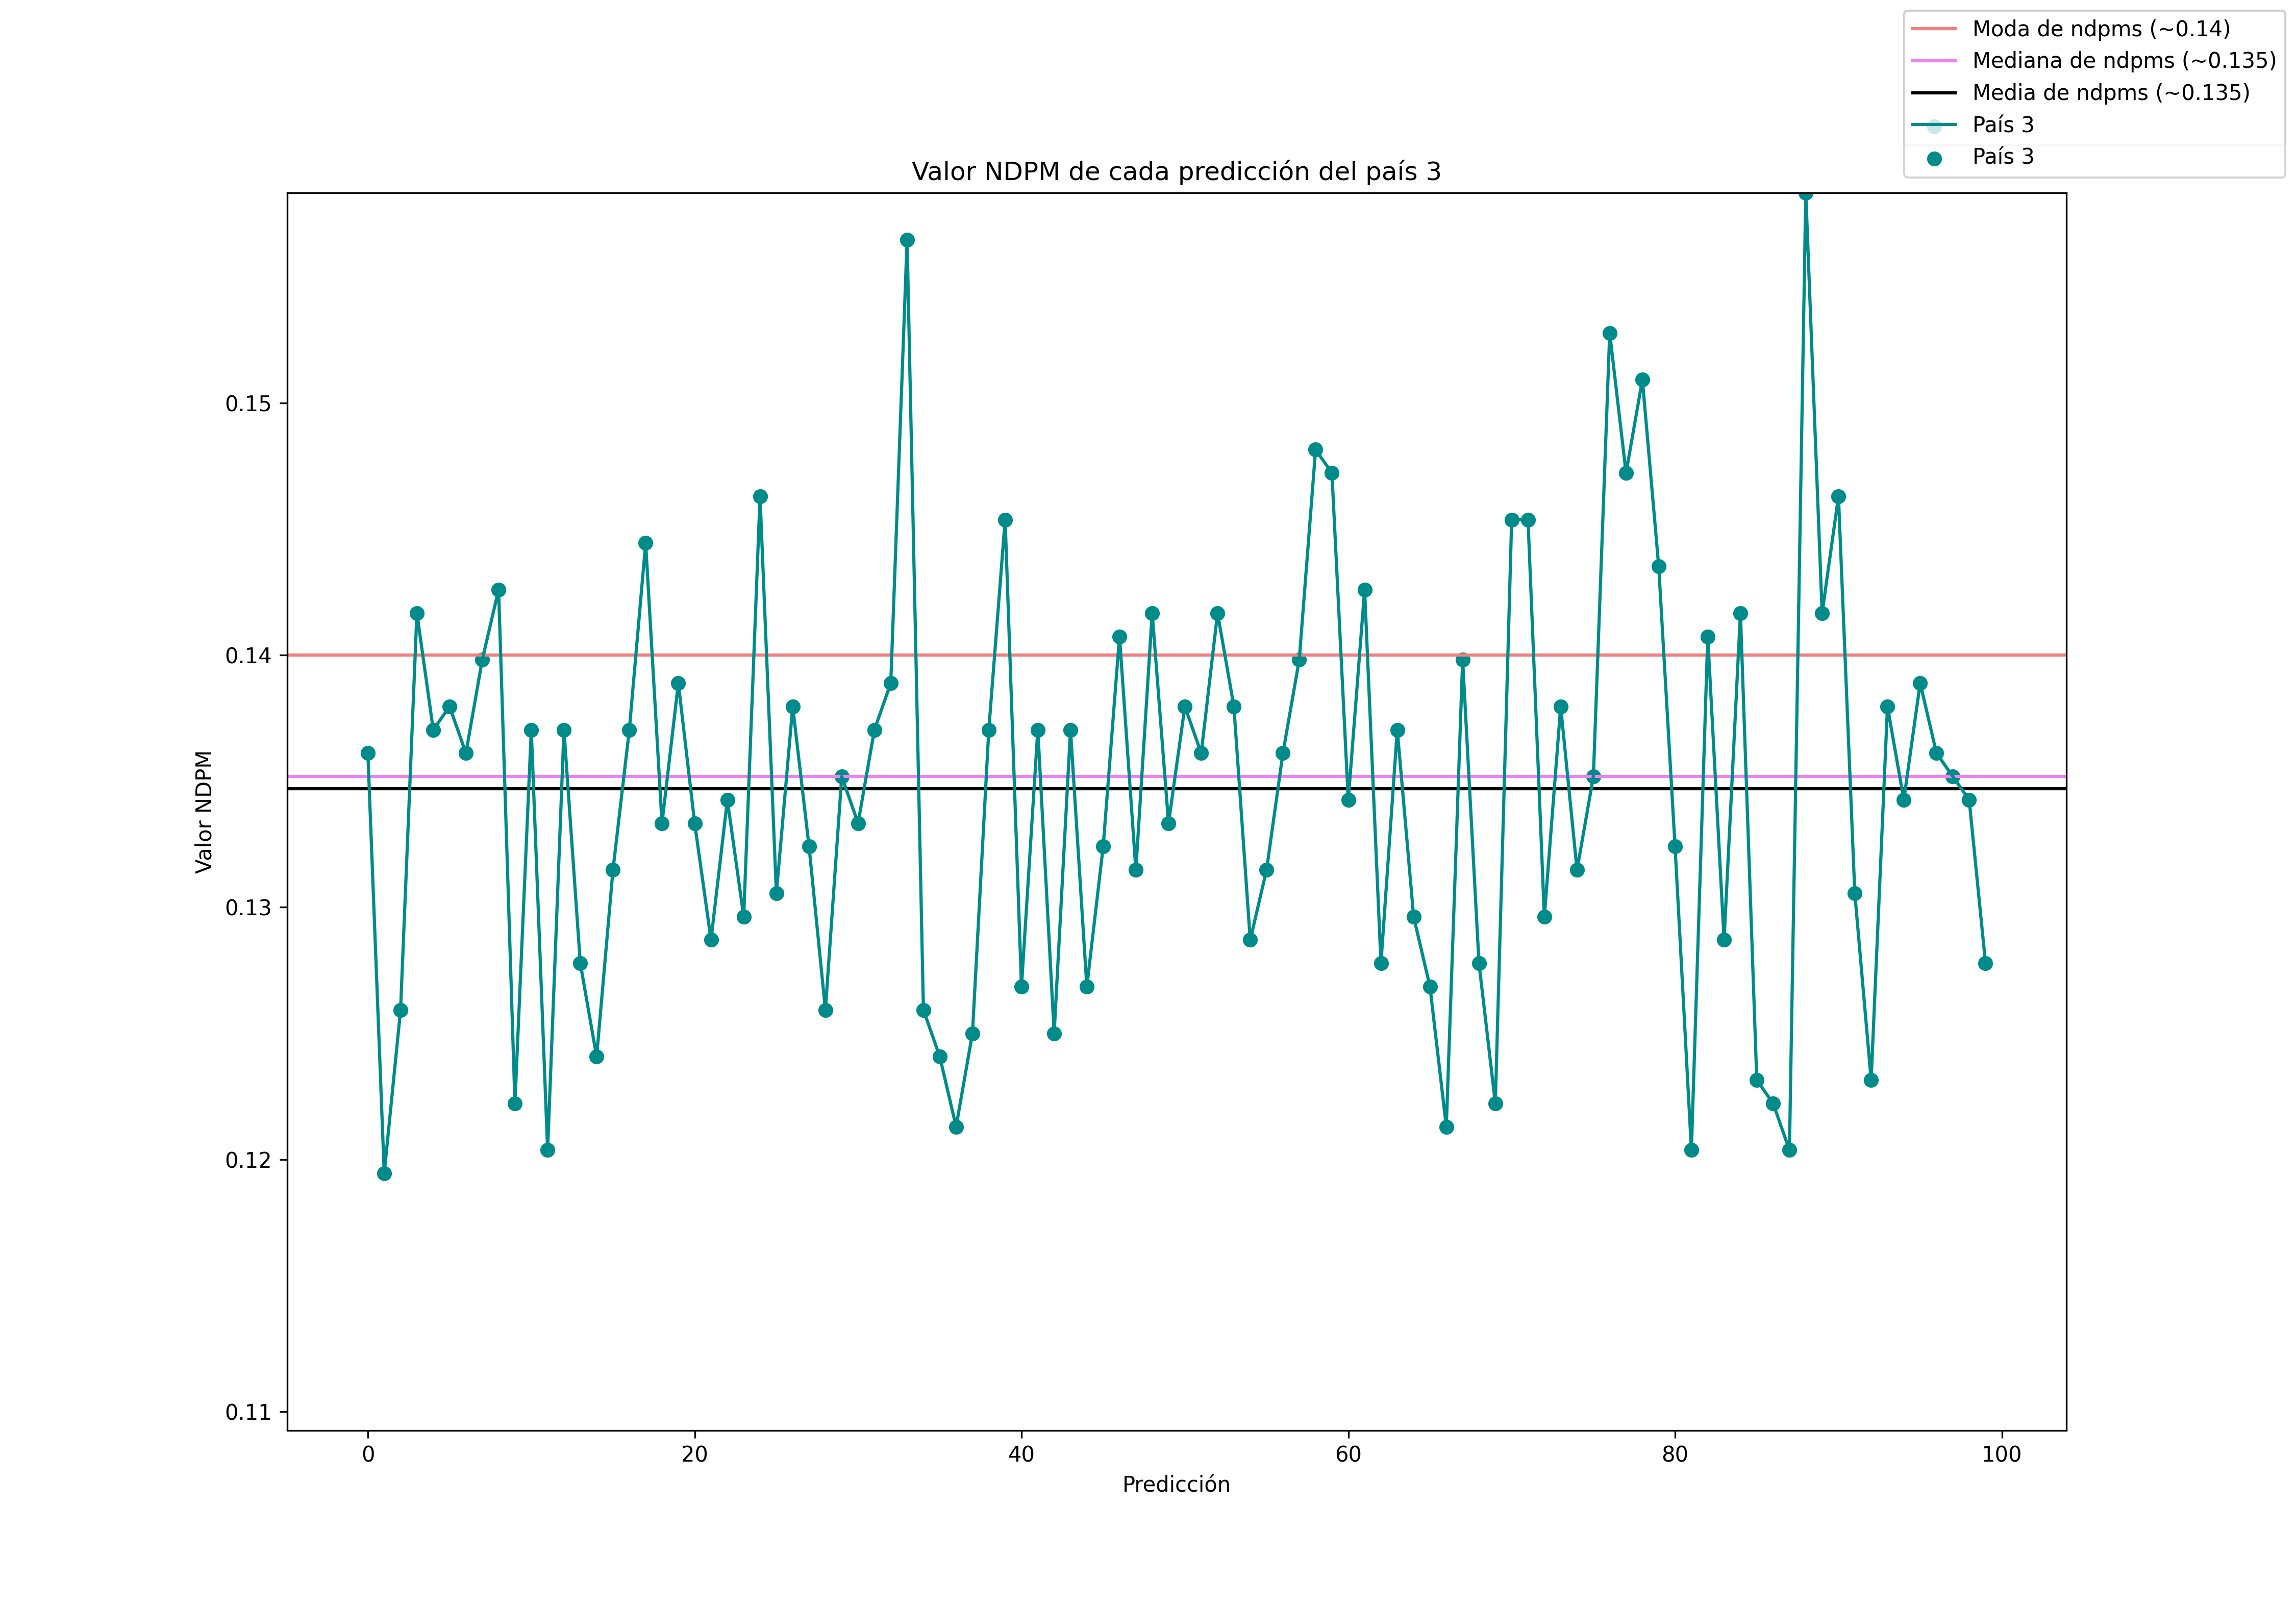
\includegraphics[width=0.5\textheight]
        {Figuras/Reports/PI_3_W1_EXT_DISP.png}}
    \caption{Gráfico de los valores NDPM del participante 3\label{fig:PI3_DISP}}
\end{sidewaysfigure}
\clearpage

\begin{sidewaysfigure}
    \centering
    \subfloat[Modelo original]
        {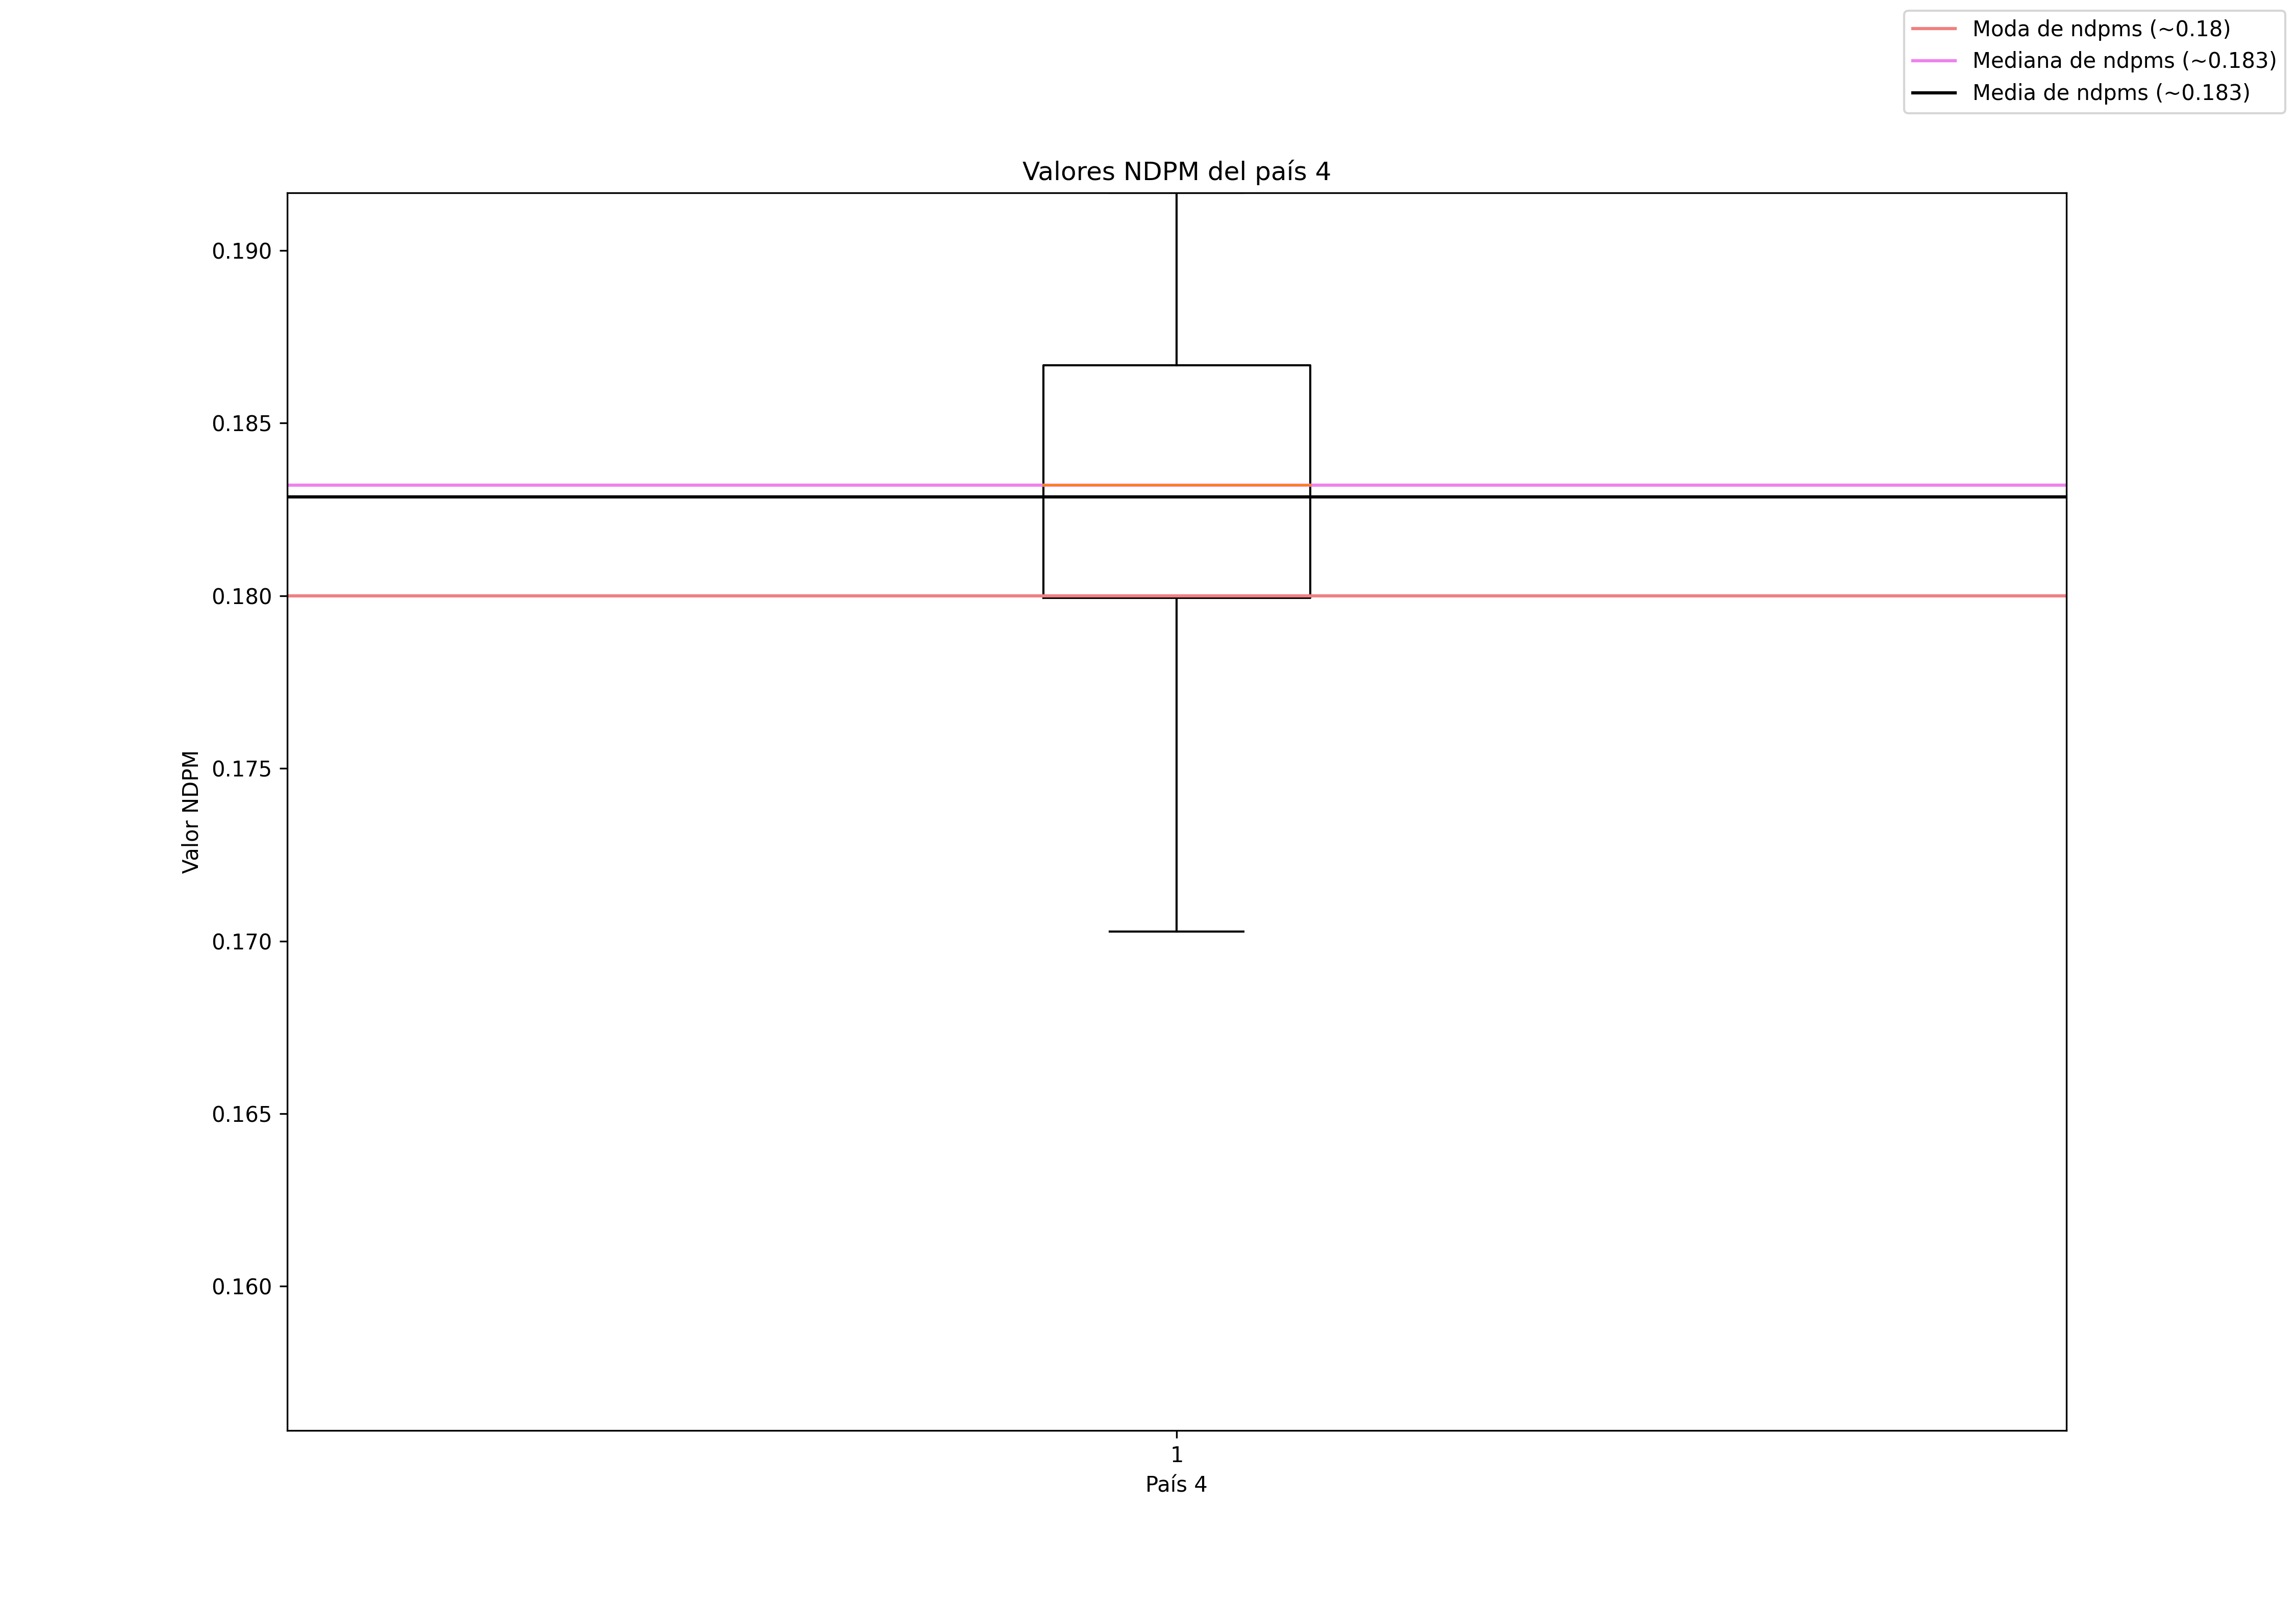
\includegraphics[width=0.5\textheight]
        {Figuras/Reports/PI_4_W0_LOC_CAJAS.png}}
        \quad
    \subfloat[Reentrenado con \textit{W$_c$ $=0$}]
        {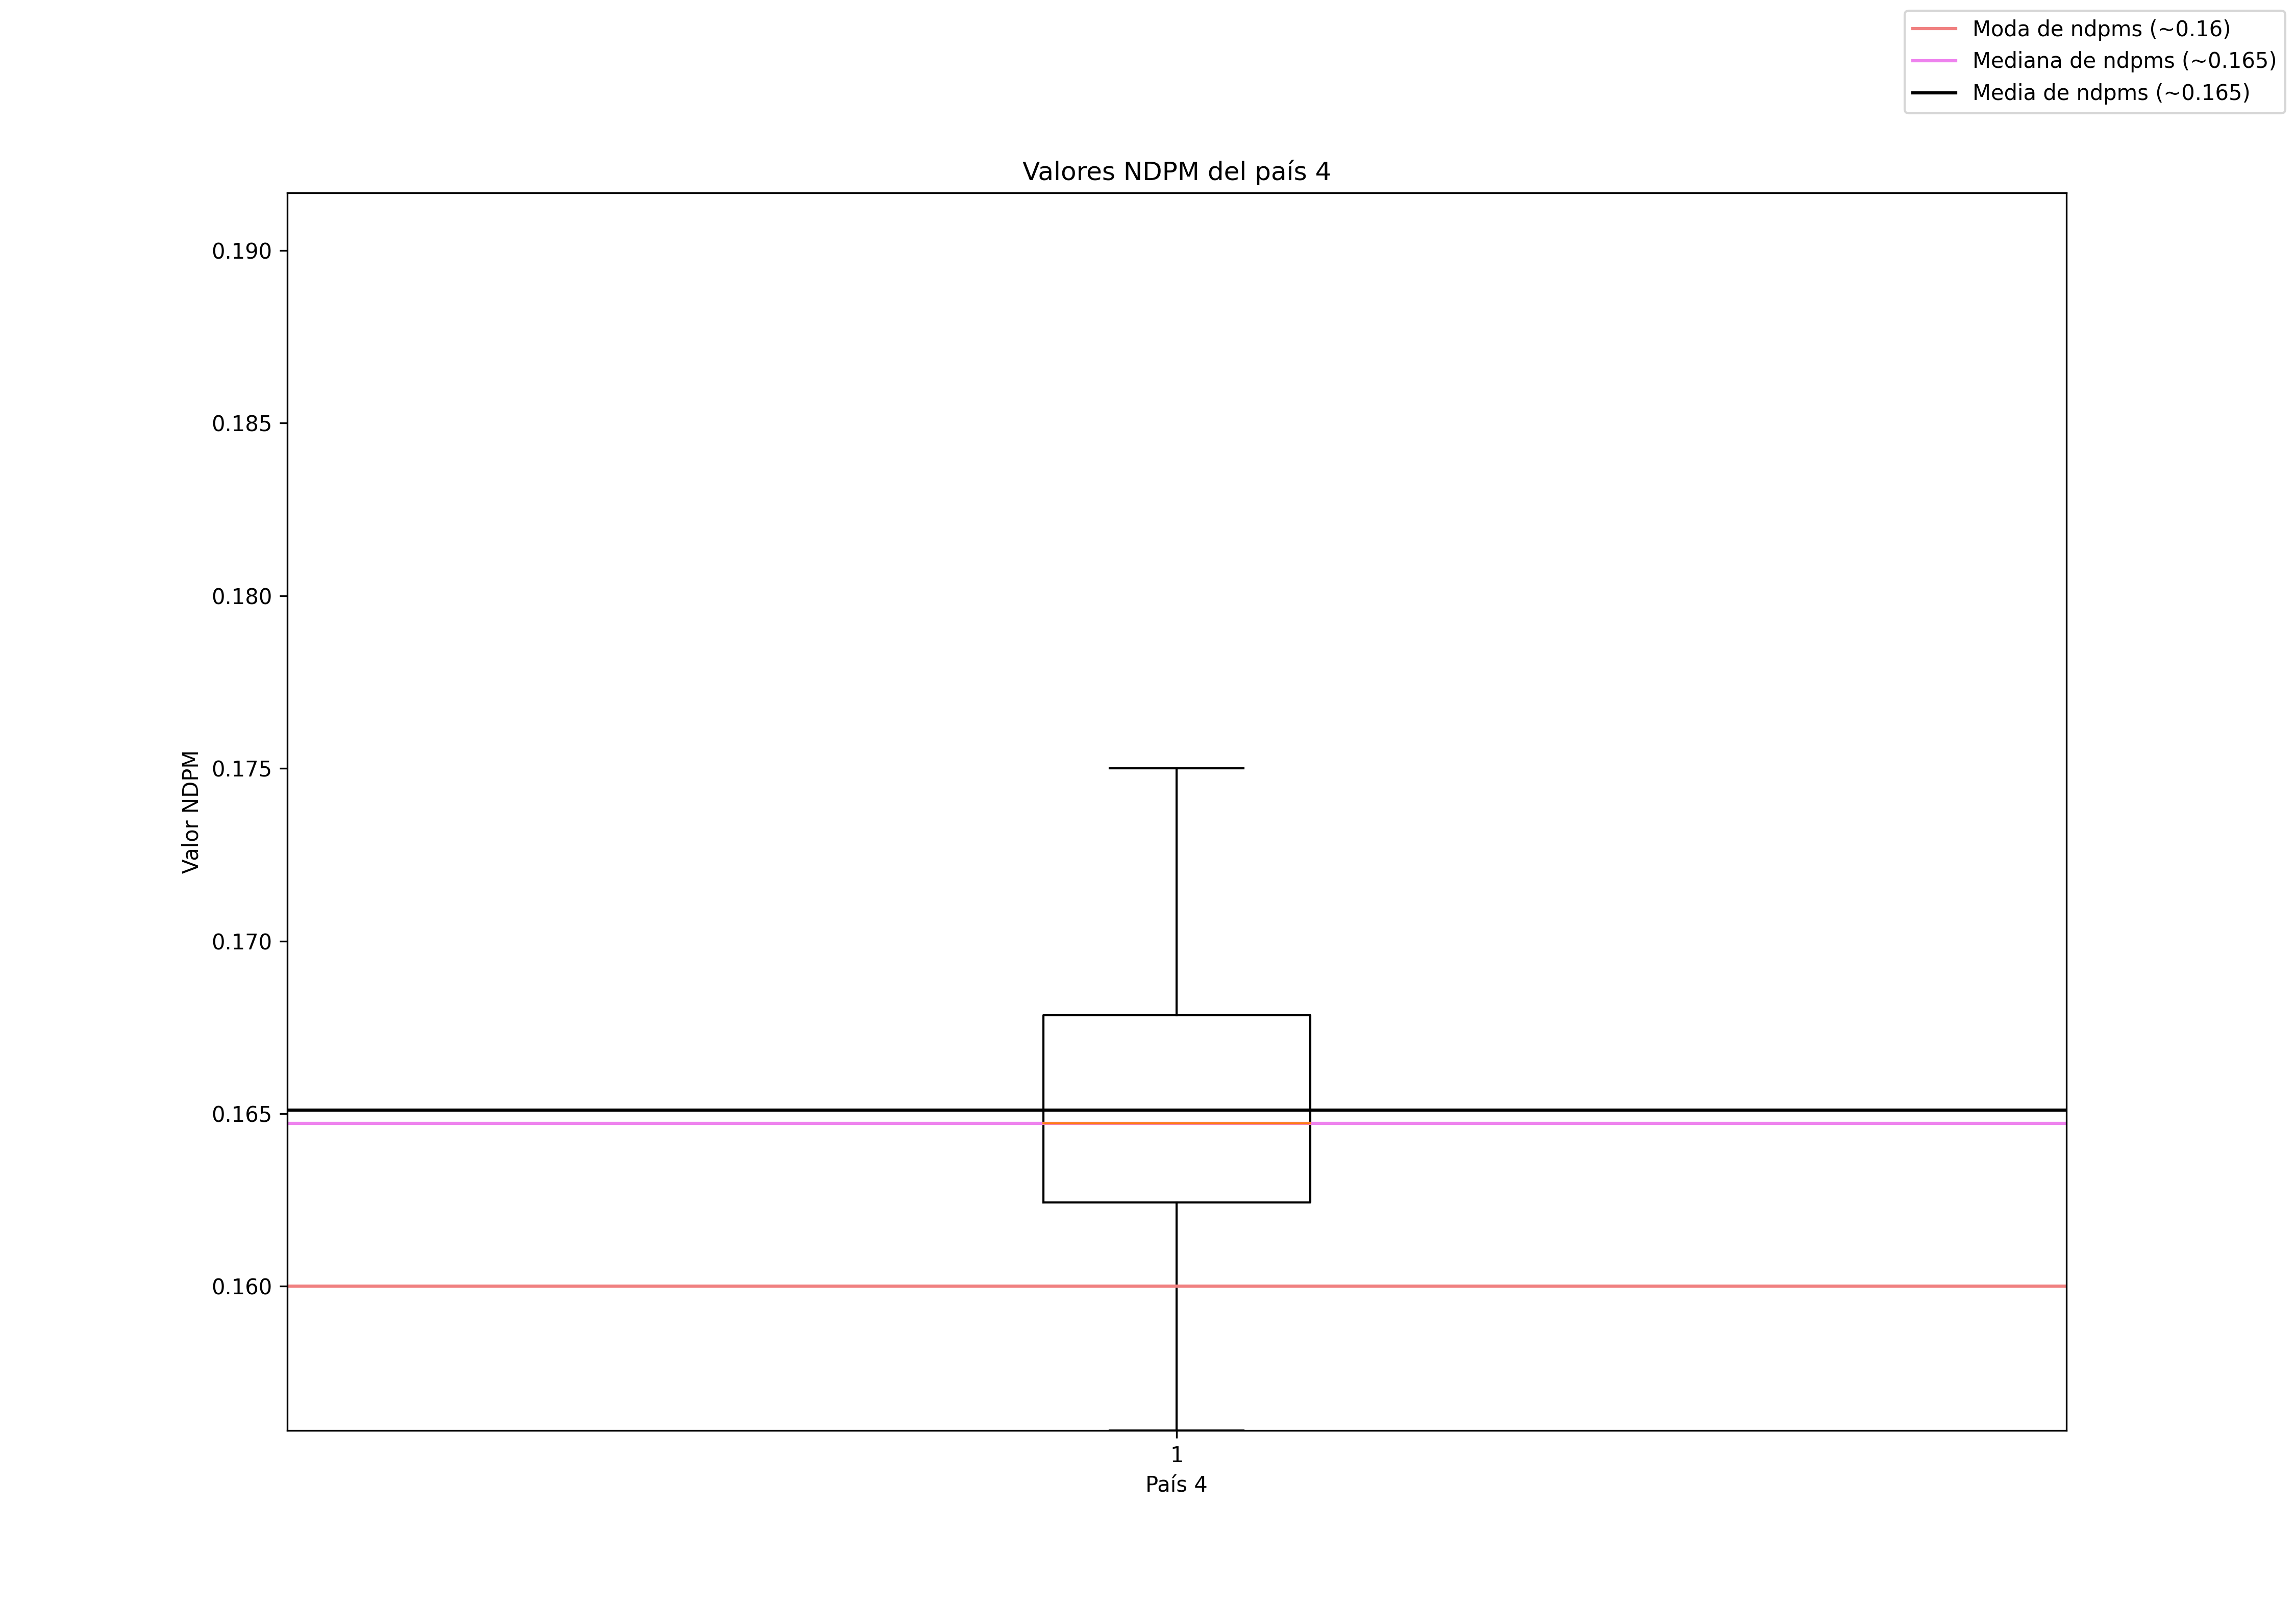
\includegraphics[width=0.5\textheight]
        {Figuras/Reports/PI_4_W0_EXT_CAJAS.png}}
    \subfloat[Reentrenado con \textit{W$_c$ $=1$}]{
        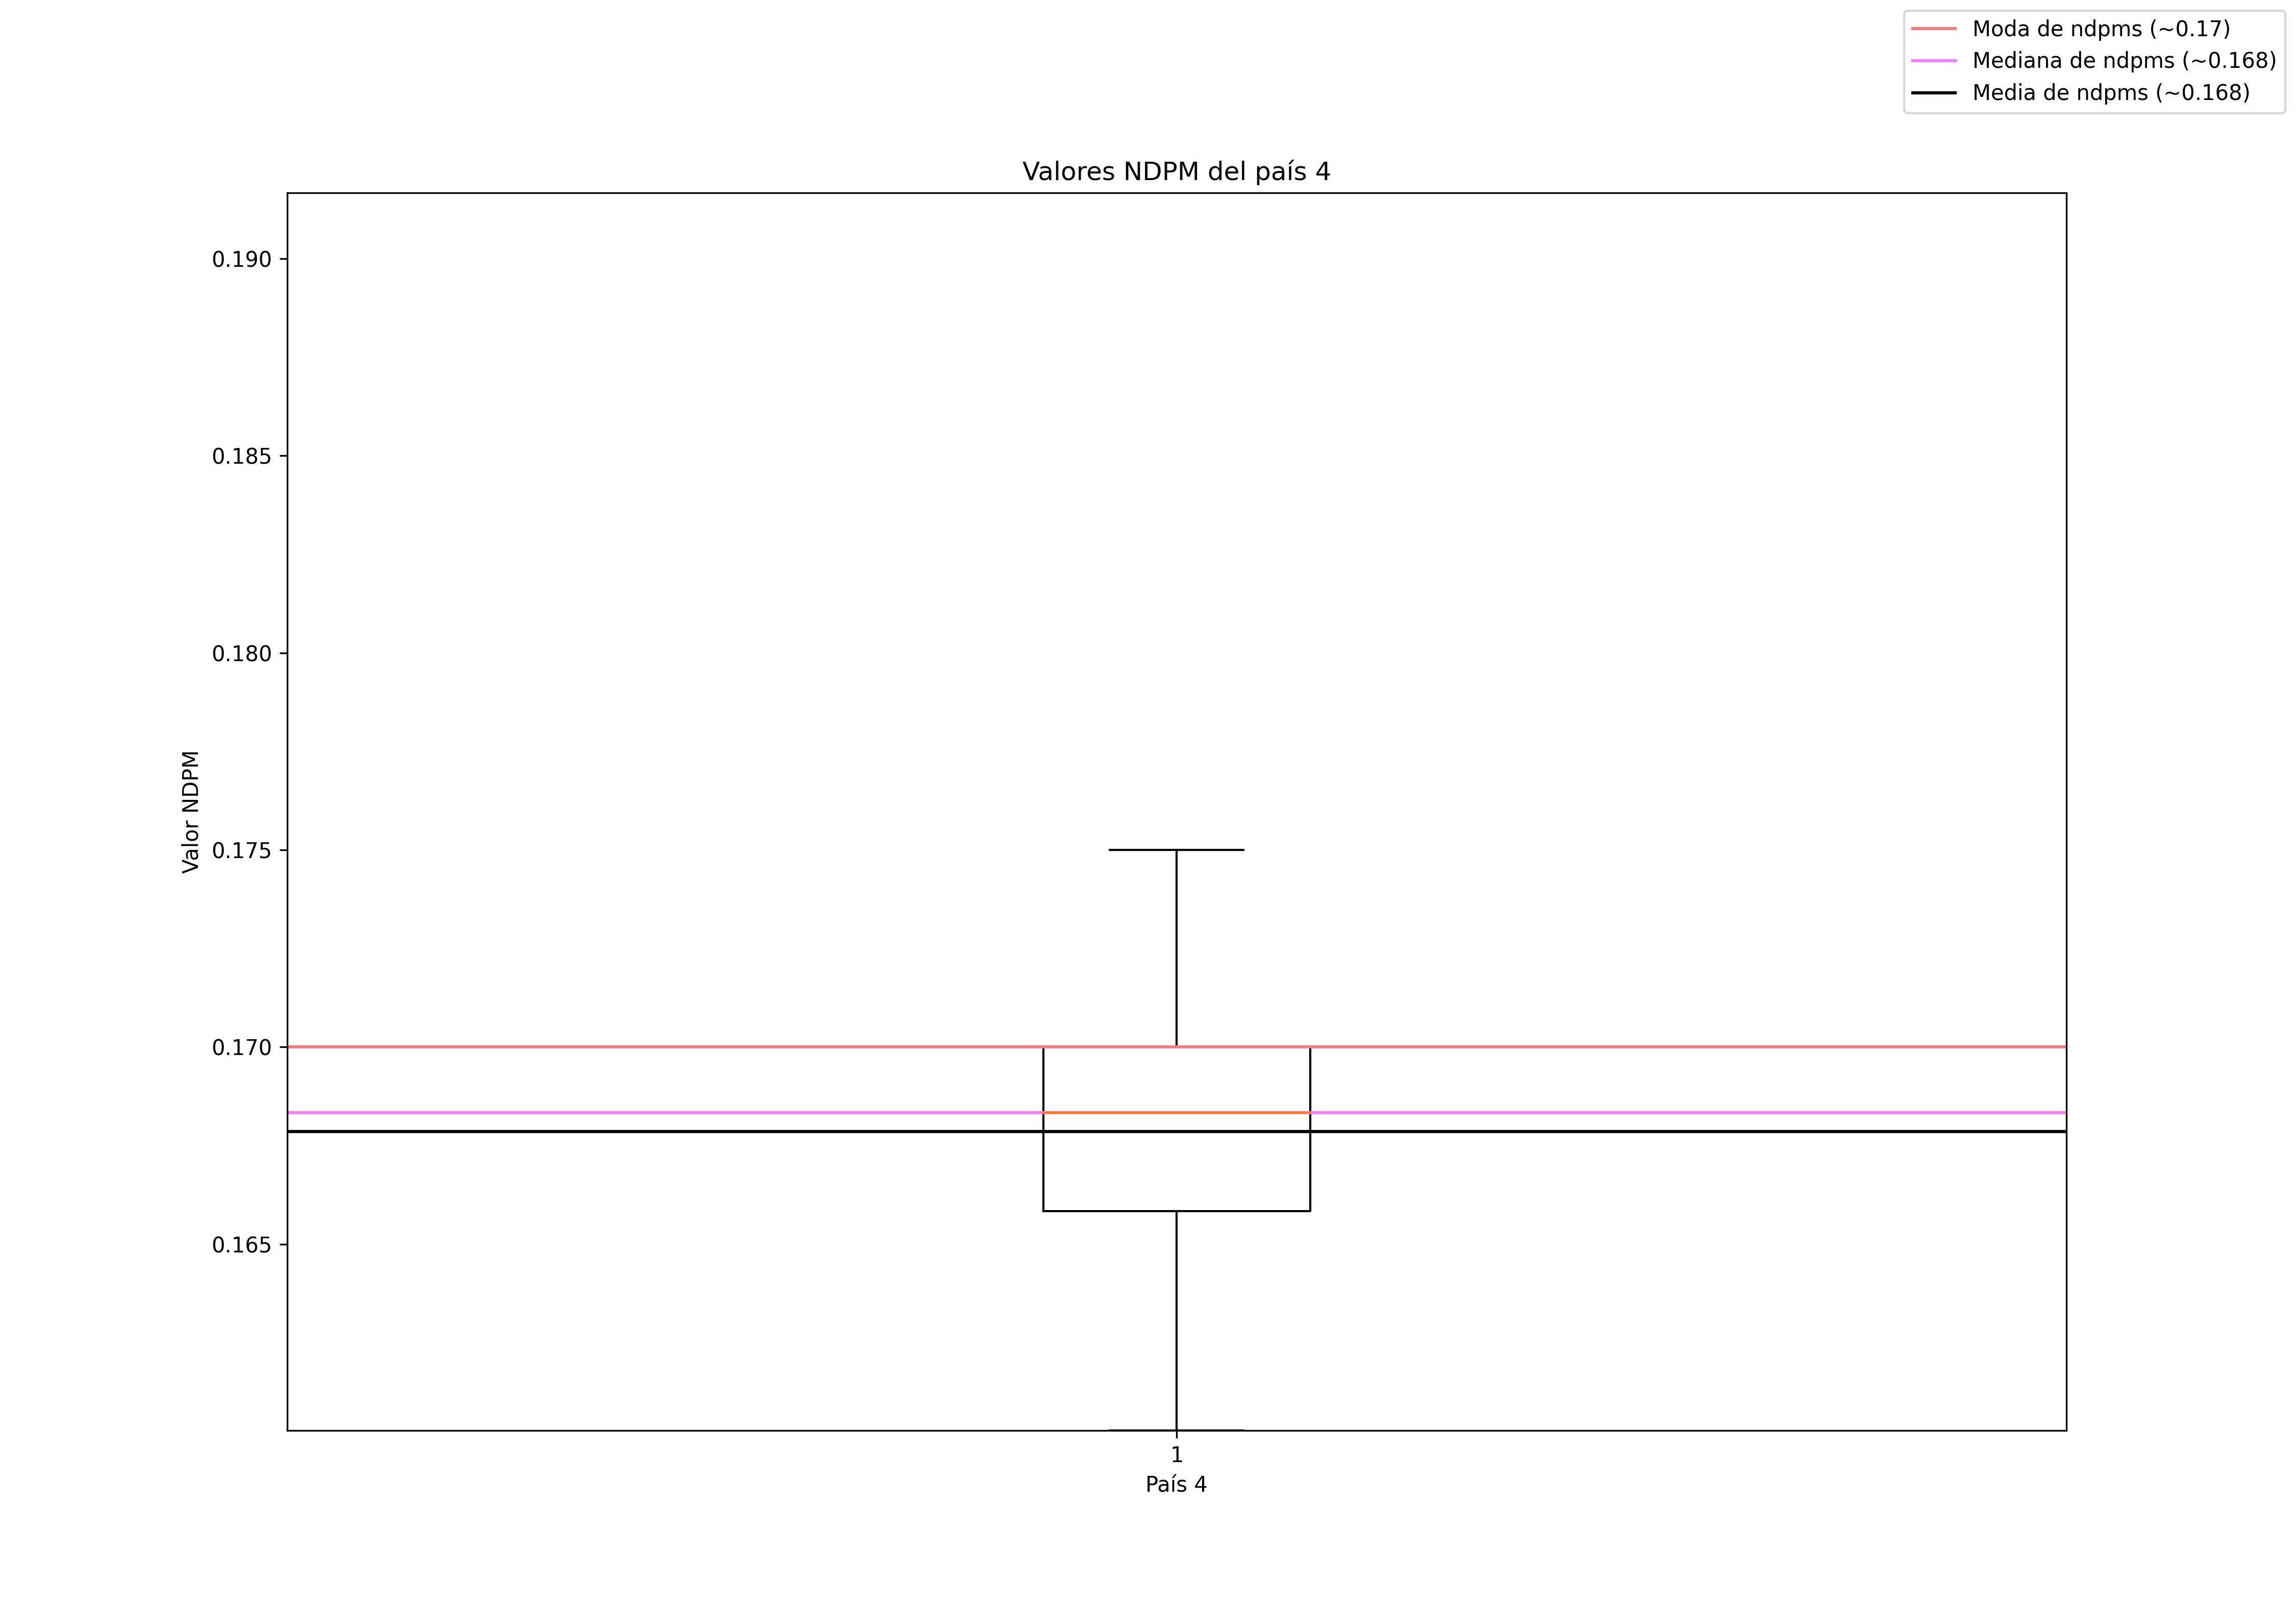
\includegraphics[width=0.5\textheight]
        {Figuras/Reports/PI_4_W1_EXT_CAJAS.png}}
    \caption{Diagramas de cajas y bigotes de los valores NDPM del participante 4\label{fig:PI4_CAJAS}}
\end{sidewaysfigure}
\clearpage
\begin{sidewaysfigure}
    \centering
    \subfloat[Modelo original]
        {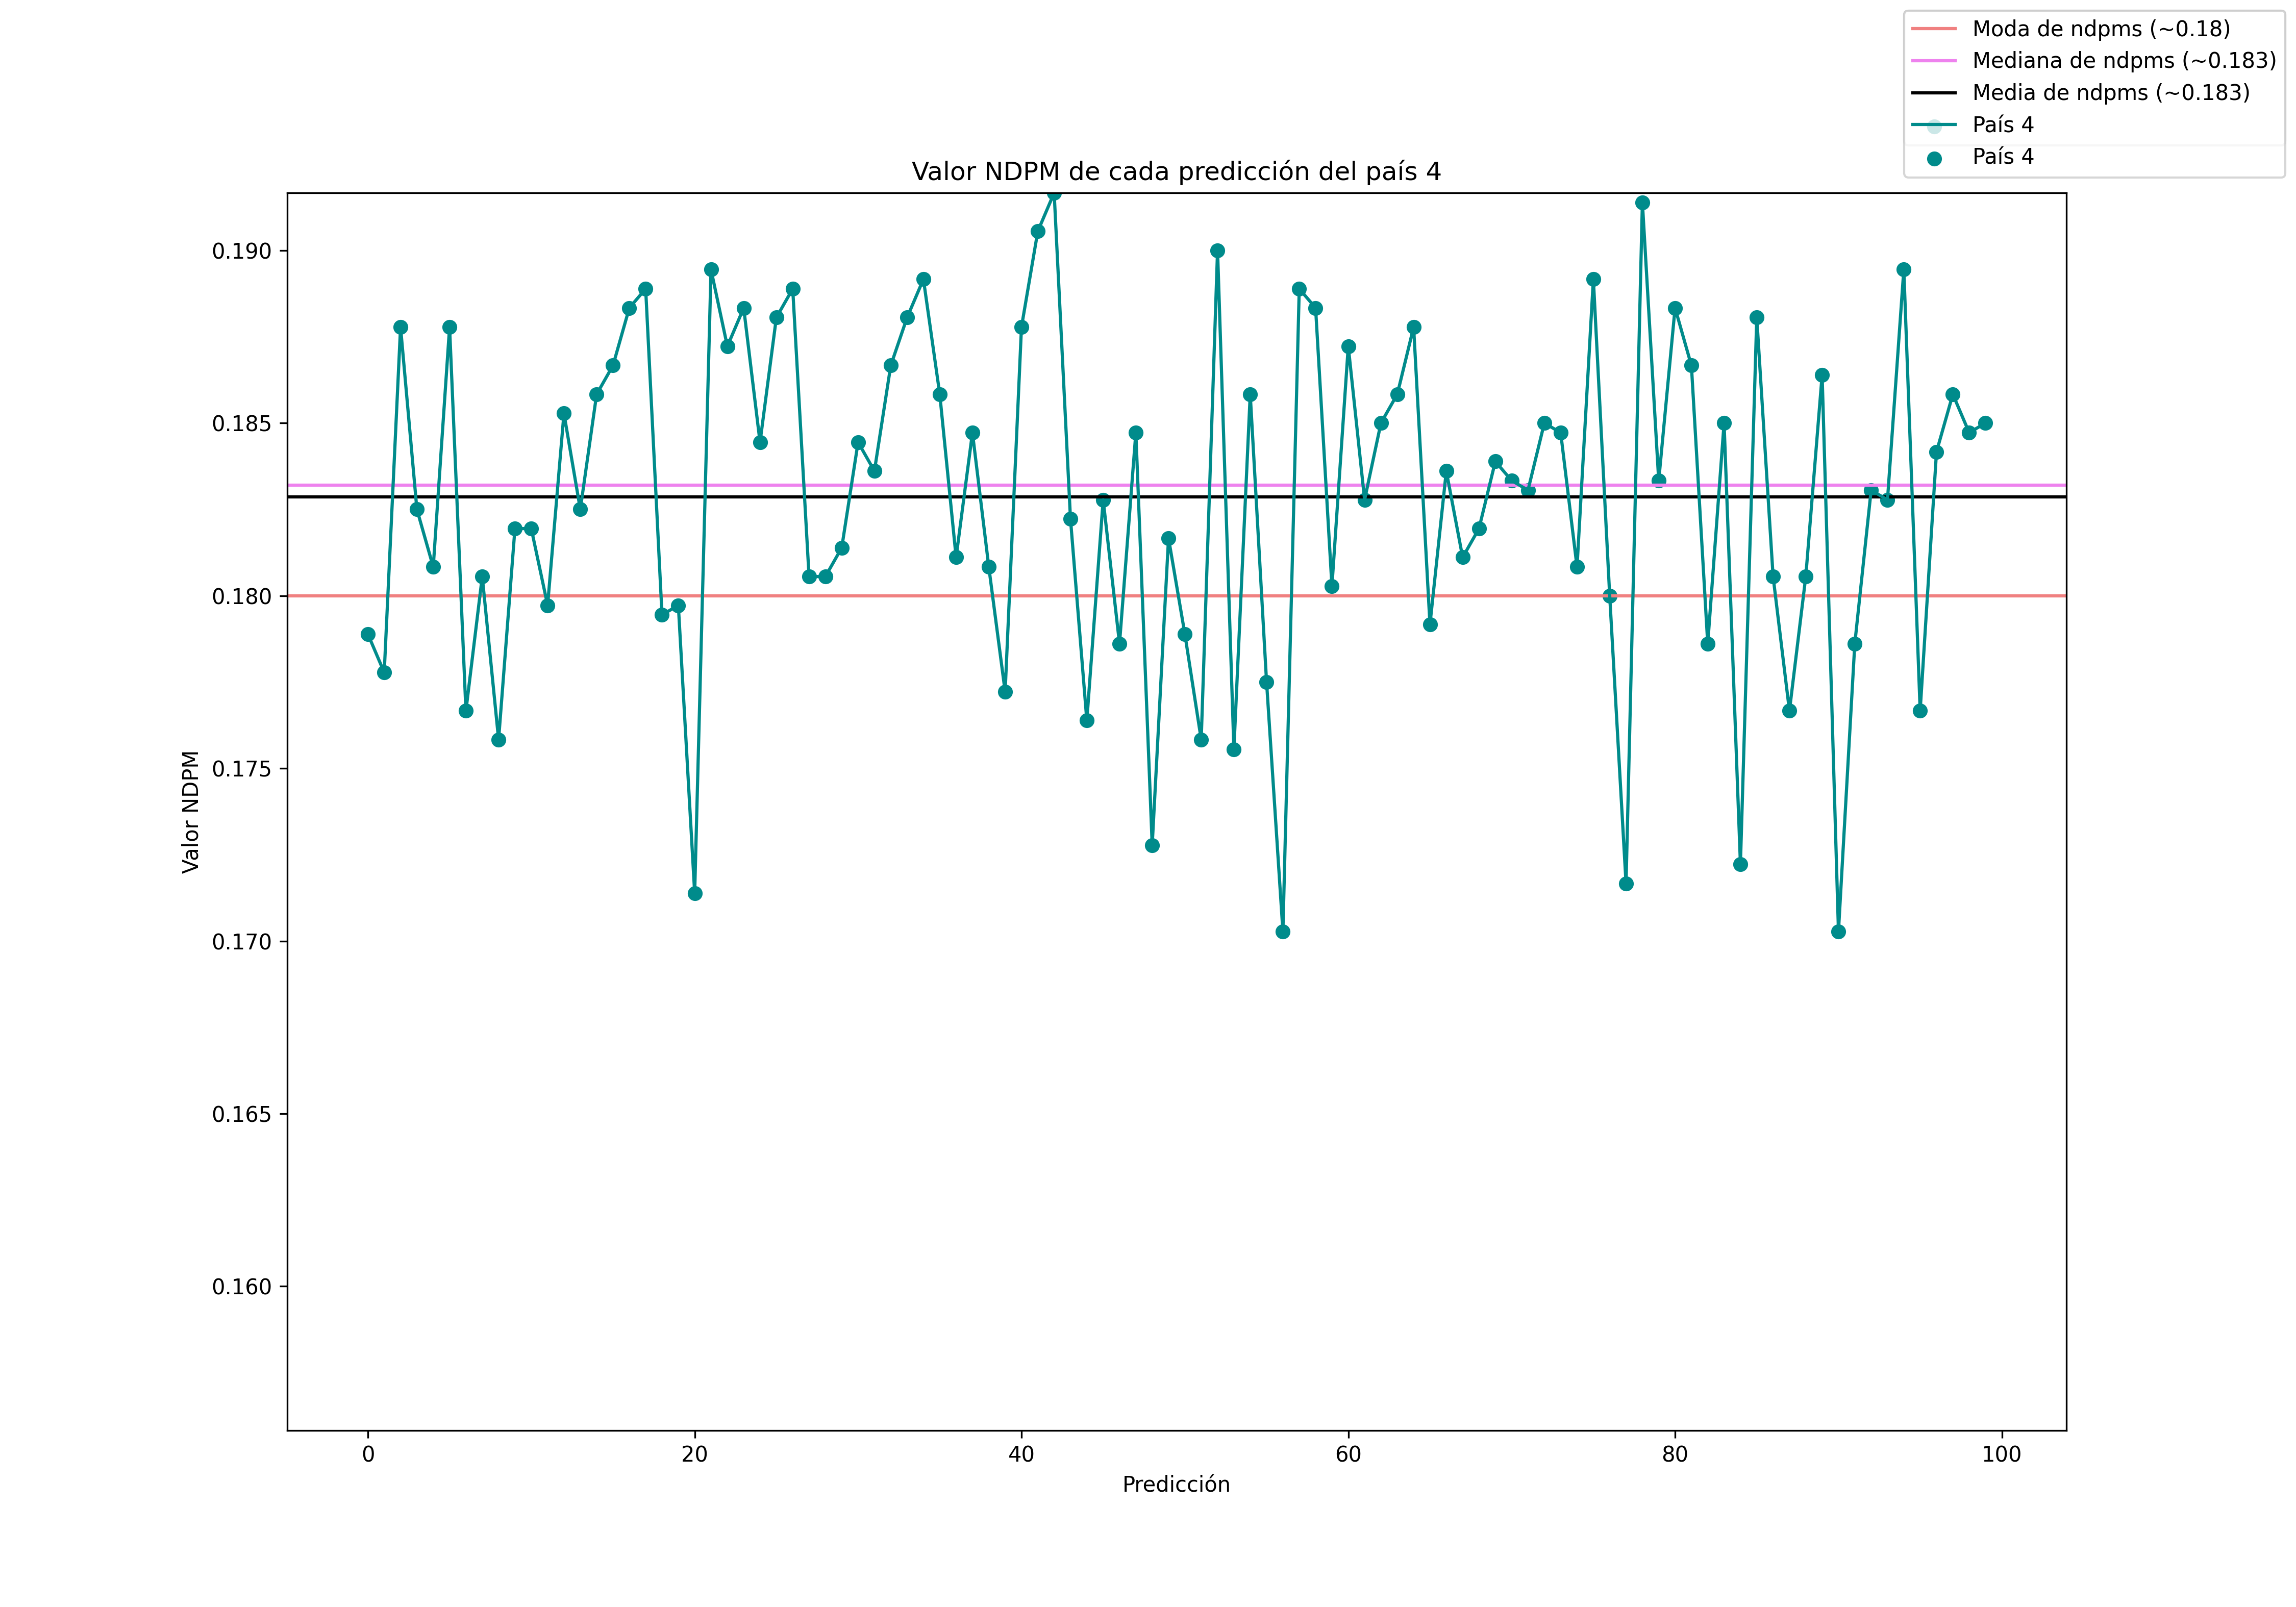
\includegraphics[width=0.5\textheight]
        {Figuras/Reports/PI_4_W0_LOC_DISP.png}}
        \quad
    \subfloat[Reentrenado con \textit{W$_c$ $=0$}]
        {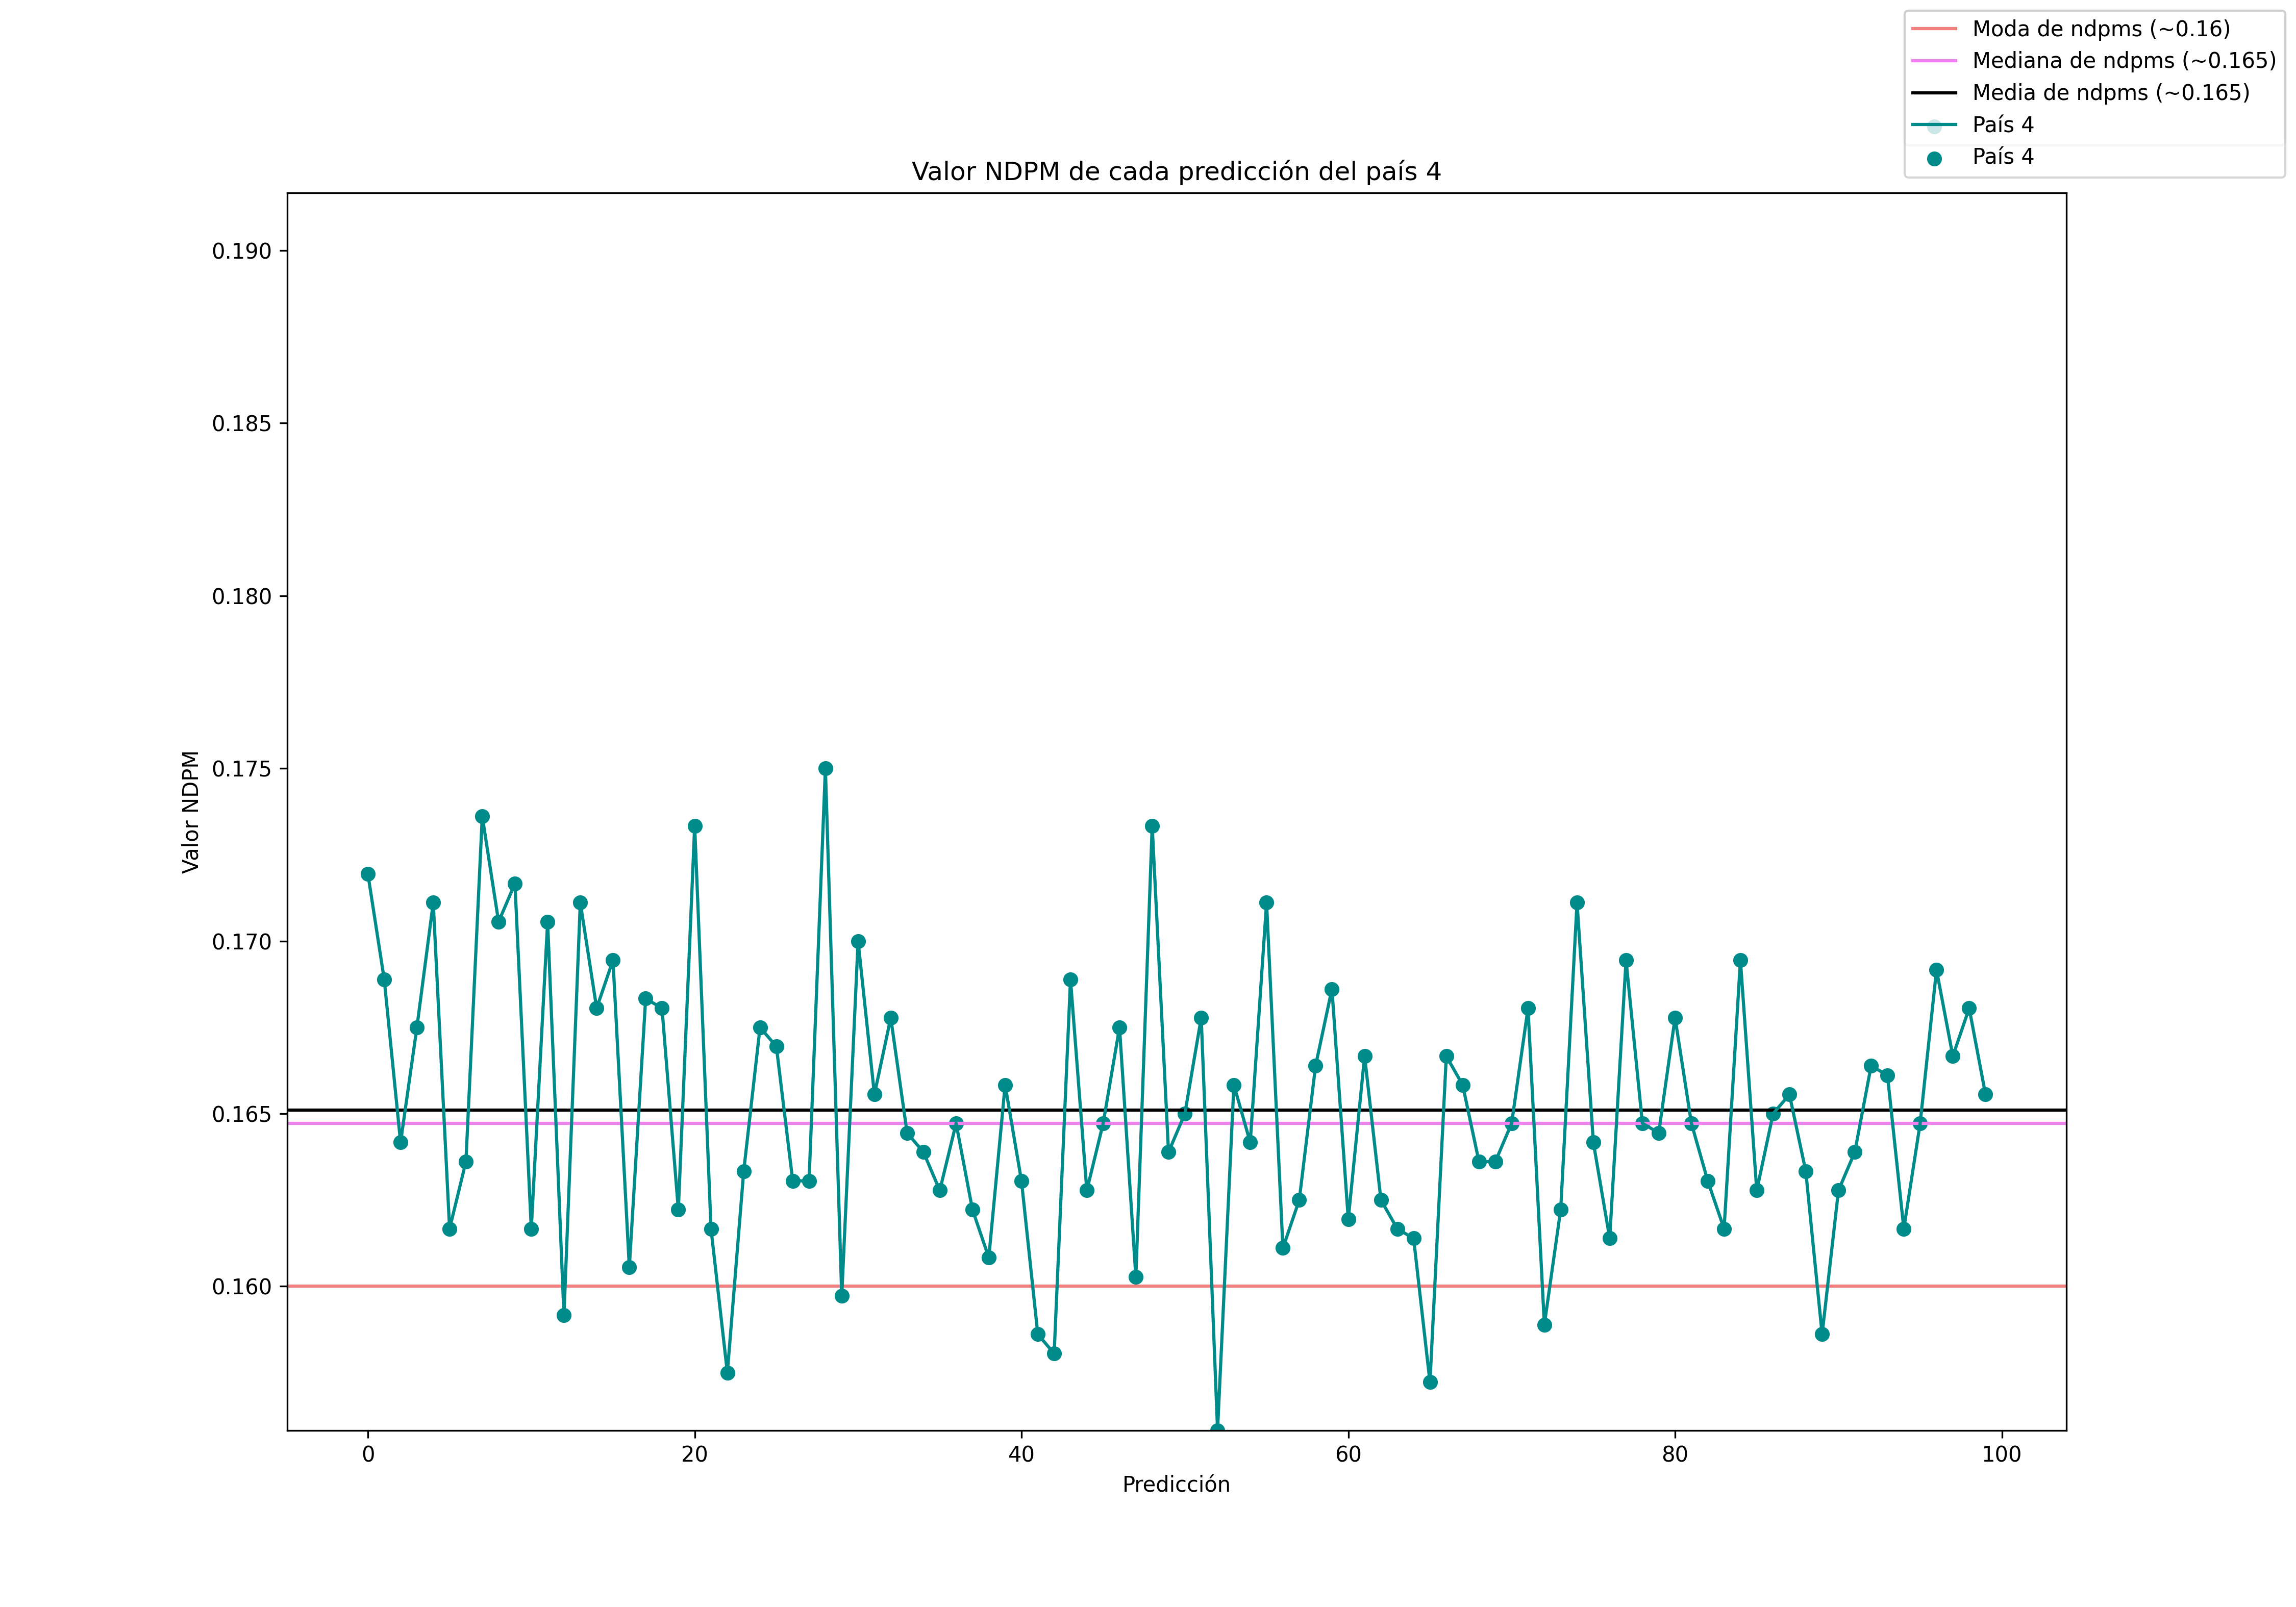
\includegraphics[width=0.5\textheight]
        {Figuras/Reports/PI_4_W0_EXT_DISP.png}}
    \subfloat[Reentrenado con \textit{W$_c$ $=1$}]{
        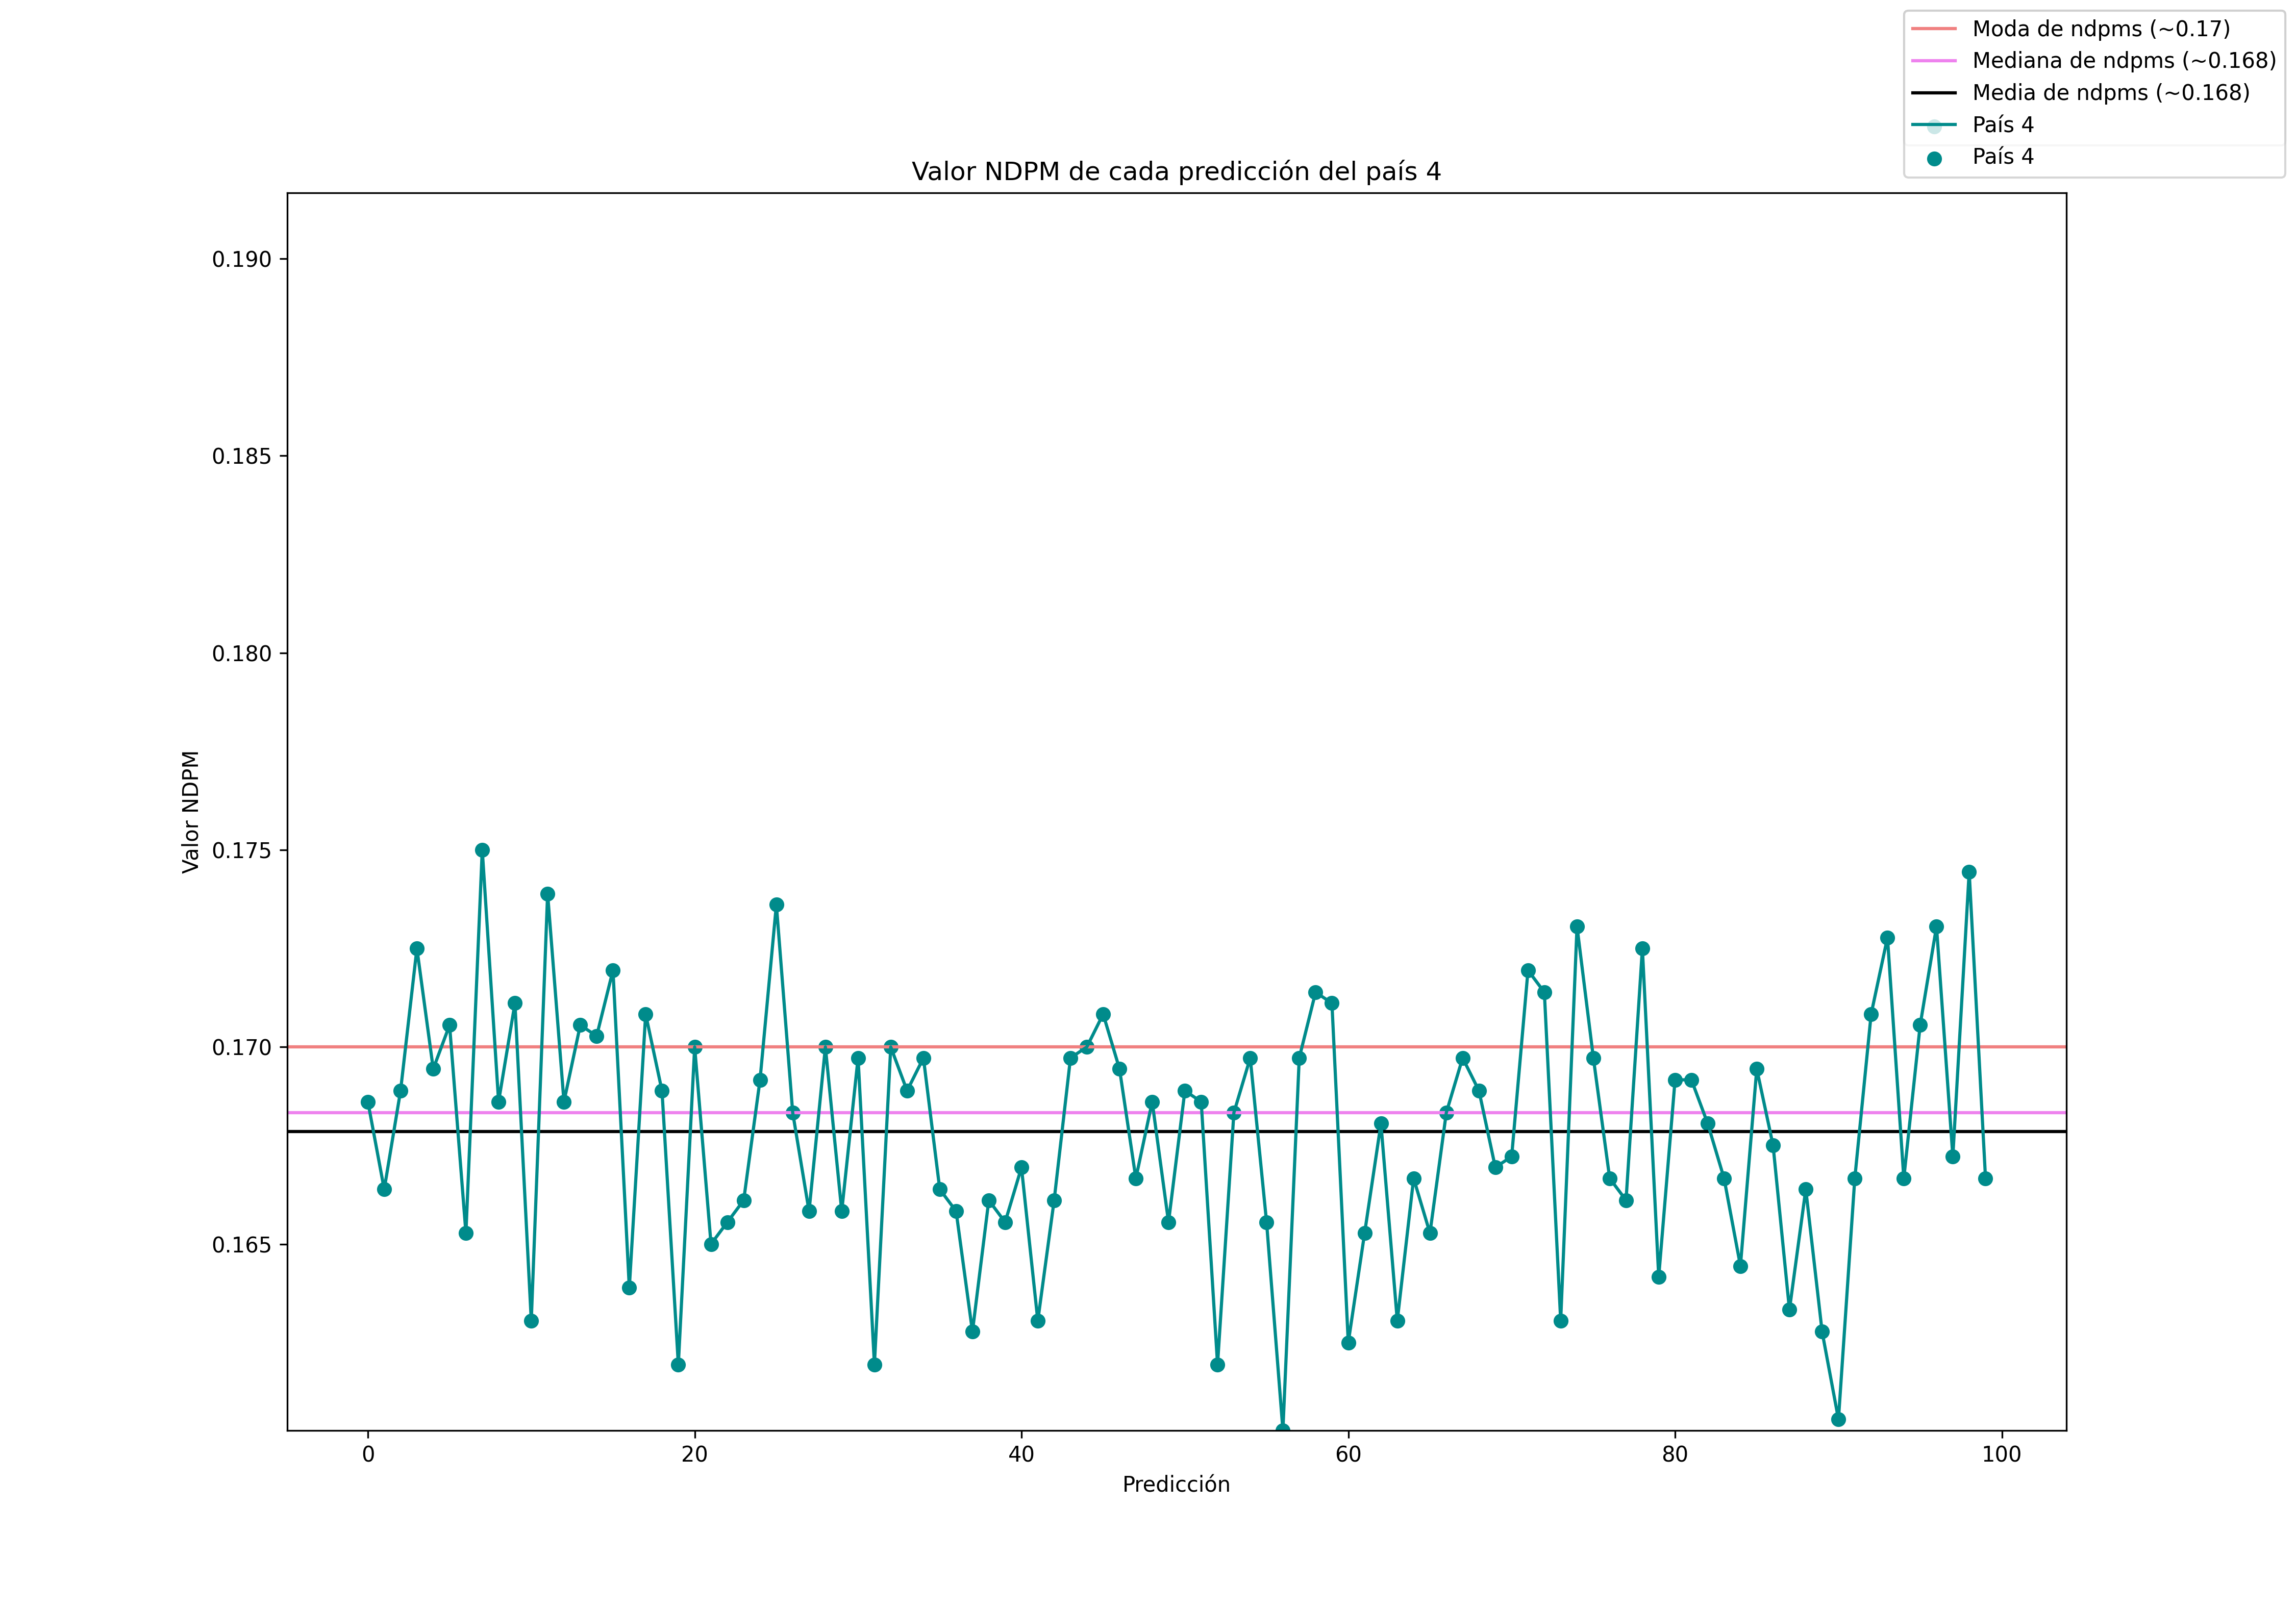
\includegraphics[width=0.5\textheight]
        {Figuras/Reports/PI_4_W1_EXT_DISP.png}}
    \caption{Gráfico de los valores NDPM del participante 4\label{fig:PI4_DISP}}
\end{sidewaysfigure}
\clearpage




\subsubsection{Conclusiones}
Teniendo en cuenta lo anteriormente mencionado, podría decirse que este sistema permite que los participantes que cuentan con pocos datos se beneficien del conocimiento de otros usuarios, aunque estos no se vean compensados en ocasiones. Con cada iteración del protocolo el conocimiento pasa a ser más homogéneo a lo largo de los participantes. Además, con la introducción de nuevos datos en cada participante se consigue un sistema sostenible en el tiempo.
\\ \\
Las diferencias que plantea el FL sobre el ML convencional pueden resultar en ocasiones beneficiosas, en este caso, debido a la heterogeneidad de los datos, la segregación de modelos es beneficiosa. En ocasiones, cada grupo de usuarios necesita su propio modelo porque un modelo global les perjudica, como es el caso del participante 1 en la tabla \ref{tab:NDPM_PARTICIPANTE_1}. El caso es que el participante 1 en el sistema FL de información descentralizada es capaz de elaborar predicciones con más precisión que un RS con información centralizada, su participación en el sistema de FL permite que participantes que tendrían peores resultados que el RS convencional mejoren bastante su rendimiento. Esto se puede ver claramente en las tablas \ref{tab:NDPM_PARTICIPANTES_COLOR_W0} y \ref{tab:NDPM_PARTICIPANTES_COLOR_W1}, donde todos los participantes consiguen resultados mucho mejores que el RS convencional, siendo el participante 4 el único que se acerca al rendimiento del RS convencional por debajo. 
\\ \\
En este caso queda claro que la heterogeneidad de los RSs en ocasiones perjudica a un sistema centralizado y beneficia a un sistema distribuido. 